% This is samplepaper.tex, a sample chapter demonstrating the
% LLNCS macro package for Springer Computer Science proceedings;
% Version 2.21 of 2022/01/12
%
\documentclass[runningheads]{llncs}
%
\usepackage[T1]{fontenc}
% T1 fonts will be used to generate the final print and online PDFs,
% so please use T1 fonts in your manuscript whenever possible.
% Other font encondings may result in incorrect characters.
%
\usepackage{graphicx}
% Used for displaying a sample figure. If possible, figure files should
% be included in EPS format.
%
% If you use the hyperref package, please uncomment the following two lines
% to display URLs in blue roman font according to Springer's eBook style:
%\usepackage{color}
%\renewcommand\UrlFont{\color{blue}\rmfamily}
%\urlstyle{rm}
%

\usepackage{amsmath}
%\usepackage{amsthm}
%\usepackage[dvipdfmx]{graphicx}
\graphicspath{{./eps_files/}}
%\usepackage[dvipdfmx]{color}
\usepackage[colorlinks=true, allcolors=blue]{hyperref}
\usepackage{comment}
\usepackage{amssymb}
\usepackage{mathrsfs}
\usepackage{algorithmic}
\usepackage{algorithm}
\usepackage{ifthen}
\usepackage{enumitem}
\usepackage[title]{appendix}
\usepackage{here}
\newboolean{Draft}
\newboolean{Draft2}
\setboolean{Draft}{true} %図を挿入するならtrue
\setboolean{Draft2}{false} %付録を挿入するならtrue

\begin{comment}
\theoremstyle{plain}
%\newtheorem{theorem}{Theorem}
\newtheorem{theorem*}{Theorem}
%\newtheorem{proposition}{Proposition}
\newtheorem{subroutine}{Subroutine}
%\newtheorem{lemma}{Lemma}
\newtheorem{cor}{Corollary}
\theoremstyle{definition}
%\newtheorem{definition}{Definition}
\newtheorem{definition}{Definition}
\end{comment}
\newtheorem{cor}{Corollary}



\begin{document}
%
\title{Designing various algorithms based on DAG-pathwidth}
%
%\titlerunning{Abbreviated paper title}
% If the paper title is too long for the running head, you can set
% an abbreviated paper title here
%
\begin{comment}
\author{First Author\inst{1}\orcidID{0000-1111-2222-3333} \and
Second Author\inst{2,3}\orcidID{1111-2222-3333-4444} \and
Third Author\inst{3}\orcidID{2222--3333-4444-5555}}
%
\authorrunning{F. Author et al.}
% First names are abbreviated in the running head.
% If there are more than two authors, 'et al.' is used.
%
\institute{Princeton University, Princeton NJ 08544, USA \and
Springer Heidelberg, Tiergartenstr. 17, 69121 Heidelberg, Germany
\email{lncs@springer.com}\\
\url{http://www.springer.com/gp/computer-science/lncs} \and
ABC Institute, Rupert-Karls-University Heidelberg, Heidelberg, Germany\\
\email{\{abc,lncs\}@uni-heidelberg.de}}


\author{Jun Kawahara\inst{1}\orcidID{0000-0001-7208-044X} \and
Shinya Izu\inst{1}\orcidID{1111-2222-3333-4444}}
%
\authorrunning{J. Kawahara et al.}
% First names are abbreviated in the running head.
% If there are more than two authors, 'et al.' is used.
%
\institute{Princeton University, Princeton NJ 08544, USA \and
Springer Heidelberg, Tiergartenstr. 17, 69121 Heidelberg, Germany
\email{lncs@springer.com}\\
\url{http://www.springer.com/gp/computer-science/lncs} \and
ABC Institute, Rupert-Karls-University Heidelberg, Heidelberg, Germany\\
\email{\{abc,lncs\}@uni-heidelberg.de}}
\end{comment}


\author{Shinya Izu\inst{1} \and
Jun Kawahara\inst{1}\orcidID{0000-0001-7208-044X}}
%
\authorrunning{Shinya Izu and Jun Kawahara}
%
\institute{Yoshida Honmachi, Sakyo-ku, Kyoto, 606--8501, Japan
\email{\{izu.shinya.54w@st,jkawahara@i\}.kyoto-u.ac.jp}}

%
\maketitle              % typeset the header of the contribution
%
\begin{abstract}
%The abstract should briefly summarize the contents of the paper in 150--250 words.

DAG (Directed Acyclic Graph)-pathwidth is a parameter that measures how closely a directed graph is to a directed path. This parameter is useful for designing parameterized algorithms to solve NP-hard problems even on DAGs.
%This parameter provides a non-trivial width even for DAG, which is difficult to parameterize with directed pathwidth. 

In this paper, we first design parameterized algorithms with DAG-pathwidth for various NP-hard problems even on DAGs. Specifically, we design fixed-parameter tractable (FPT) algorithms for the \textsc{Directed Dominating Set Problem} and the \textsc{Max Leaf Outbranching Problem}. Given a DAG with $n$ vertices and a DAG-path-decomposition of width $w$, both problems can be solved exactly in $O(2^w w n)$ time. Similarly, we propose parameterized algorithms for the \textsc{Directed Steiner Tree Problem} and the \textsc{$k$-Disjoint Path Problem}. 

Next, we show the existence of a polynomial-time approximation algorithm for DAG-pathwidth that achieves an $O(\log^{3/2} n)$ approximation ratio by demonstrating the equivalence between constructing DAG-path-decomposition and solving one-shot Black Pebbling game. 

%It is known that computing the DAG-pathwidth is NP-hard, and, to our knowledge, no algorithm has been known for finding small DAG-pathwidth. In this paper, 
We also design an algorithm that, given an integer $t$ and DAG $H$ with $l$ roots and at most $d$ outdegree, either computes a DAG-path-decomposition of $H$ with width $O(l d^t)$ or provides evidence that the DAG-pathwidth of $H$ is greater than $t$.

%For the Directed Steiner Tree Problem, where the terminal set size is $k$, we propose an FPT algorithm that computes an exact solution in $O(2^w (k + w)n + n^2)$ time. For the $k$-Disjoint Path Problem, we develop a parameterized algorithm that computes an exact solution in $O((k+1)^w (w^2 + k)n + n^2)$ time.

%Finally, we define a new parameter DAG-treewidth as a generalization of DAG-pathwidth. DAG-treewith is a parameter that measures how similar is the structure of a directed graph to that of a directed tree. We show that constructing an optimal DAG-tree-decomposition that minimizes DAG-treewidth is NP-hard. After that, we design an FPT algorithm for the Directed Dominating Set Problem in $O(2^w w^2 n)$ time, with the DAG-treewidth $w$ as a parameter.

\keywords{Graph algorithm \and Computational complexity \and Directed acyclic
graph \and Pathwidth.}
\end{abstract}
%
%
%
\section{Introduction}

\emph{Path} and \emph{tree decompositions}~\cite{art1,art2} are prominent techniques for efficiently solving NP-hard problems on graphs. These methods transform the input graph into a path-like or tree-like structure, enabling the extension of dynamic programming algorithms originally designed for paths or trees to more general graph classes. The effectiveness of these decompositions is characterized by their width: \emph{pathwidth} for path decompositions and \emph{treewidth} for tree decompositions. A smaller pathwidth/treewidth indicates that the graph's structure is closer to a path/tree. When the width is bounded by a constant, it is sometimes possible to solve NP-hard problems in polynomial time with respect to the number of vertices.

For directed graphs, \emph{directed pathwidth} was introduced by Reed~\cite{art9}, and \emph{directed treewidth} by Johnson et al.~\cite{art10}. Berwanger et al.~\cite{art11} proposed a width parameter, called \emph{DAG-width}, specifically for directed acyclic graphs (DAGs). DAG-width measures how close a directed graph is to a DAG. However, if the input graph is a DAG, this parameter is always at most one, making it difficult to construct parameterized algorithms for NP-hard problems on DAGs.

%Kasahara et al.~\cite{art12} proposed \emph{DAG-pathwidth}, which measures how close a directed graph is to a directed path. DAG-pathwidth adds a rule requiring that for any edge, its endpoints must appear in the same bag of the decomposition. This ensures that strongly connected components are contained in a single bag, allowing non-trivial widths for DAGs and facilitating effective FPT algorithm design.

Kasahara et al.~\cite{art12} proposed \emph{DAG-pathwidth}, which measures how close a directed graph is to a directed path. DAG-path decompositions follow the same rules as standard path decompositions, with the added constraint that for any vertex, its first appearance in a bag must respect the topological order of the original input graph, and all vertices within a strongly connected component of the original graph must appear together in one bag. This constraint facilitates the design of efficient fixed-parameter tractable (FPT) algorithms especially on DAGs. While they introduced DAG-pathwidth to analyze the discord $k$-independent set problem, we believe that this concept has broader applicability and can be a valuable tool for analyzing various NP-hard problems on DAGs. Although they demonstrated that computing DAG-pathwidth is NP-hard, they did not provide a practical algorithm for its computation.

%Tree decomposition is one of the approach to efficiently solve NP-hard problems. This operation is dividing the vertices of a undirected graph into subsets, treating each subset as a node, and transforming the graph into a tree-like structure. This enables algorithms designed for trees to general graphs, which allows efficient solutions even for NP-hard problems. Each node in a tree decomposition is called bag, and the \emph{width} of the tree decomposition is the maximum number of vertices in a single bag. A \emph{treewidth} is the minimum width across all possible tree decompositions of a graph. A smaller treewidth indicates that the graph's structure is closer to a tree. When the treewidth is bounded by a constant, it is sometimes possible to solve NP-hard problems in polynomial time with respect to the number of vertices.

%Similarly, \emph{path decomposition} transforms a graph into a path-like structure by partitioning its vertices into subsets. Like treewidth, \emph{pathwidth} is the minimum width across all possible path decompositions. A path decomposition also enables efficient algorithms for NP-hard problems when the pathwidth is bounded by a constant.

%The pathwidth of an undirected graph was first proposed by Robertson et al.~\cite{art1}. They also introduced the concept of treewidth~\cite{art2}. Arnborg et al.~\cite{art3} later demonstrated that it is NP-complete to determine whether the treewidth and pathwidth of a graph is at most \(k\). They also studied various fixed-parameter tractable (FPT) algorithms using these parameters~\cite{art4}. It is unknown there exists a polynomial-time algorithm computing a tree decomposition with a width at most any constant factor of treewidth $k$. Similarly, it is also unclear whether constant-factor approximations for pathwidth are achievable. However, Amir~\cite{art5} proposed a polynomial-time algorithm that approximates treewidth within a factor of $O(\sqrt{\log k})$. Tuukka~\cite{art6} also proposed a 2-approximation algorithm with a time complexity of $2^{O(k)}$. Similarly, for pathwidth, Carla et al.~\cite{art7} proposed a polynomial-time algorithm with an approximation ratio of $O(k\sqrt{\log k})$, where \( k \) is the treewidth. In addition, Cattell et al.~\cite{art8} presented a polynomial-time algorithm that computes a path decomposition with a width of $O(2^{pw})$ , where $pw$ is the pathwidth.

%For directed graphs, several width parameters have been proposed. \emph{Directed pathwidth} was introduced by Reed in 1997~\cite{art9}, and \emph{directed treewidth} by Johnson et al.~in 2001~\cite{art10}. In 2012, Berwanger et al.~\cite{art11} proposed width parameters specifically for directed acyclic graphs (DAGs). Directed pathwidth measures how close a directed graph is to a DAG. However, for DAGs, this parameter is always at most one, making it challenging to construct parameterized algorithms for NP-hard problems on DAGs. In response, Kasahara et al.~\cite{art12} proposed \emph{DAG-pathwidth} in 2023, which measures how close a directed graph is to a directed path. DAG-pathwidth adds a rule requiring that for any edge, its endpoints must appear in the same bag of the decomposition. This ensures that strongly connected components are contained in a single bag, allowing non-trivial widths for DAGs and facilitating effective FPT algorithm design.

%In \cite{art12}, they constructed a parameterized algorithm for the discord $k$-independent set problem using DAG-pathwidth and proved that computing the DAG-pathwidth is NP-hard. On the other hand, to the best of our knowledge, it has not been developed so far to construct parameterized algorithms for the other NP-hard problems, as well as to compute a DAG-path-decomposition of small width.

%Our contributions are as follows:  
Based on the above, our contributions are as follows:  
\begin{enumerate}
    %\item Constructing parameterized algorithms using DAG-pathwidth for various NP-hard problems on DAGs.  
    \item We construct parameterized algorithms using DAG-pathwidth for various NP-hard problems on DAGs.  
    %\item Proposing approximation algorithms for DAG-path-decomposition and parameterized algorithms to construct decompositions with small width.  
    \item We propose approximation algorithms for DAG-path-decomposition and parameterized algorithms to construct decompositions with small width.  
    %\item Extending DAG-pathwidth to DAG treewidth, a parameter measuring the similarity of a directed graph to a directed tree.  
    %\item We newly extend DAG-pathwidth to DAG-treewidth, a parameter measuring the similarity of a directed graph to a directed tree.  
\end{enumerate}

%In Section 3, we design FPT algorithms for the \textsc{Directed Dominating Set Problem} and the \textsc{Max Leaf Outbranching Problem} on DAGs in $O(2^w wn)$ time, given a DAG with $n$ vertices and a DAG-path-decomposition of width $w$. We also design an FPT algorithm for the \textsc{Directed Steiner Tree Problem}, which runs in $O(2^w(k + w)n + n^2)$ time when the size of the terminal set is $k$. Additionally, we propose a parameterized algorithm for the \textsc{$k$-Disjoint Path Problem}, which runs in $O((k + 1)^w(w^2 + k)n + n^2)$ time. At the end of Section 3, we show the advantages of DAG-pathwidth compared to treewidth using the \textsc{Directed Edge Dominating Set Problem}. While the proposed algorithms are designed for DAGs, they can also be applied to general directed graphs by performing a strongly connected component. In Section 4, we show the existence of a $O(\log^{3/2} n)$-approximation algorithm for DAG-pathwidth on DAGs by demonstrating the equivalence between the one-shot Black Pebbling Problem and the problem of computing the DAG-pathwidth. 

%Finally, in Section 5, we design an algorithm that, given an integer $t$, and a DAG with maximum outdegree $d$, number of roots $l$, provides a DAG-path-decomposition with width $O(l \cdot d^t)$. This algorithm is based on the one for undirected path decompositions \cite{art8}, and both of these algorithms utilize the graph embedding of complete trees.

In Section 3, we design FPT algorithms for the \textsc{Directed Dominating Set Problem} and the \textsc{Max Leaf Outbranching Problem} on DAGs in $O(2^w wn)$ time, given a DAG with $n$ vertices and a DAG-path-decomposition of width $w$. We also design an FPT algorithm for the \textsc{Directed Steiner Tree Problem}, which runs in $O(2^w(k + w)n + n^2)$ time when the size of the terminal set is $k$. Additionally, we propose a parameterized algorithm for the \textsc{$k$-Disjoint Path Problem}, which runs in $O((k + 1)^w(w^2 + k)n + n^2)$ time. At the end of Section 3, we show the advantages of DAG-pathwidth compared to treewidth using the \textsc{Directed Edge Dominating Set Problem}. While the proposed algorithms are designed for DAGs, they can also be applied to general directed graphs by performing a strongly connected component. In Section 4, we show the existence of an $O(\log^{3/2} n)$-approximation algorithm for DAG-pathwidth on DAGs by demonstrating the equivalence between the one-shot Black Pebbling Problem and the problem of computing the DAG-pathwidth. 
%
Finally, in Section 5, we design an algorithm that, given an integer $t$, and a DAG with maximum outdegree $d$, number of roots $l$, provides a DAG-path-decomposition with width $O(l \cdot d^t)$. This algorithm is based on the one for undirected path decompositions \cite{art8}, and both of these algorithms utilize the graph embedding of complete trees.

\vspace{4mm}
\noindent
\textbf{Related work}\quad The pathwidth of an undirected graph was first proposed by Robertson et al.~\cite{art1}. They also introduced the concept of treewidth~\cite{art2}. Arnborg et al.~\cite{art3} later demonstrated that it is NP-complete to determine whether the treewidth and pathwidth of a graph is at most \(k\). They also studied various FPT algorithms using these parameters~\cite{art4}. It is unknown there exists a polynomial-time algorithm computing a tree decomposition with a width at most any constant factor of treewidth $k$. Similarly, it is also unclear whether constant-factor approximations for pathwidth are achievable. However, Amir~\cite{art5} proposed a polynomial-time algorithm that approximates treewidth within a factor of $O(\sqrt{\log k})$. Tuukka~\cite{art6} also proposed a 2-approximation algorithm with a time complexity of $2^{O(k)}$. Similarly, for pathwidth, Carla et al.~\cite{art7} proposed a polynomial-time algorithm with an approximation ratio of $O(k\sqrt{\log k})$, where \( k \) is the treewidth. In addition, Cattell et al.~\cite{art8} presented a polynomial-time algorithm that computes a path decomposition with a width of $O(2^{pw})$ , where $pw$ is the pathwidth.




\section{Preliminaries}\label{chapter2}
%In this Section, we introduce definitions and notations for graphs and directed graphs.

%\subsection{DAG}
%A \emph{DAG} (Directed Acyclic Graph) is a directed graph with no cycles. For a DAG $G = (V, E)$ and a vertex $v \in V$ , we define the \emph{predecessors} as $\mathsf{pred}(v) = \{ u \in V | (u, v) \in E\}$ and \emph{successors} as $\mathsf{suc}(v) = \{ w \in V | (v, w) \in E\}$ of $v$.

A \emph{directed acyclic graph} (DAG) is a directed graph with no cycles. For a DAG $G = (V, E)$ and a vertex $v \in V$, we define the \emph{predecessors} as $\mathsf{pred}(v) = \{ u \in V \mid (u, v) \in E\}$ and \emph{successors} as $\mathsf{suc}(v) = \{ w \in V \mid (v, w) \in E\}$ of $v$.

In particular, a \emph{directed tree} is a DAG that has a unique vertex $r$ with an indegree of 0, and the underlying graph forms a tree.
   

%\subsection{Various Path Decompositions and Pathwidth}

%Then, we define the \emph{DAG-path-decomposition} and the \emph{DAG-pathwidth} \cite{art12}. Let $H = (V, E)$ be a directed graph. A \emph{DAG-path-decomposition} of $H$ is a sequence $X = (X_1, X_2, \dots, X_s) ~(X_i \subseteq V)$ that satisfies the following three conditions:
We define the \emph{DAG-path-decomposition} and the \emph{DAG-pathwidth} \cite{art12}. Let $H = (V, E)$ be a directed graph. A \emph{DAG-path-decomposition} of $H$ is a sequence $X = (X_1, X_2, \dots, X_s)$ $(X_i \subseteq V)$ that satisfies the following three conditions:
\begin{description}
    \item[(DPD1)] $X_1 \cup X_2 \cup \dots \cup X_s = V$.
    \item[(DPD2)] For every directed edge $(u, v) \in E$, there exists $i$ such that $u, v \in X_i$ and $v \notin X_{i-1}$. \label{original_rule}
    \item[(DPD3)] For any $i, j, k$ $(1 \leq i \leq j \leq k \leq s)$, $X_i \cap X_k \subseteq X_j$. %That is, for any vertex $v \in V$, $v$ induces exactly one non-empty directed path in $X$.
\end{description}
In (DPD2), we interpret $X_0 = \emptyset$. Therefore, a directed edge $(u, w)$ satisfies (DPD2) if $u, v \in X_1$. The \emph{width} of $X$ is defined as $\underset{i}{\max} \{ |X_i| - 1 \}$. The \emph{DAG-pathwidth} of $G$ is the minimum width over all possible DAG-path-decompositions of $G$. Note that in \cite{art12}, (DPD2) is changed into the condition that there exists $i$ such that $u, v \in X_i$ and $u \notin X_{i-1}$. In this study, we adopt the above definition for the sake of algorithmic simplicity.

%The \emph{DAG-pathwidth} of $H$ can also be defined in the same way as the pathwidth. Note that in \cite{art12}, condition~\ref{original_rule} is defined that $u, v \in X_1$ or there exists $i$ $(i \geq 2)$ such that $u, v \in X_i$ and $u \notin X_{i-1}$. In this study, we adopt the above definition for the sake of algorithmic simplicity.

The difference between (undirected) path decomposition,
directed path decomposition, and DAG-path-decomposition is the second rule. The second rule of path decomposition is ``for any edge $(u, v) \in E$, there exists an $i$ such that $u, v \in X_i$,''  while that of directed path decomposition is ``for any directed edge $(u, v) \in E$, there exist $i, j$ $(i \leq j)$ such that $u \in X_i$, $v \in X_j$.'' %We show their entire definitions in Appendix~\ref{sec:defpd}.

The DAG-pathwidth is a parameter that indicates how closely the structure of a directed graph resembles a directed path. From (DPD3), any vertex $v$ is contained in consecutive bags. Additionally, (DPD2) and (DPD3) imply that for any edge $(u, v)$, $u$ and $v$ first appear together in a single bag or $u$ appears in a bag without $v$, followed by a bag containing both $u$ and $v$. Thus, a DAG-path-decomposition can be interpreted as an operation of adding vertices to bags according to a topological order of the graph.

%Computing the DAG-pathwidth for general directed graphs is NP-hard \cite{art12}. However, it can be shown that graphs with DAG-pathwidth 1 are exactly the \emph{directed caterpillar tree}, which is a directed tree such that removing vertices with indegree 1 and outdegree 0 leaves a single directed path. The proof is in appendix.

To facilitate designing a dynamic programming-based algorithm, we define the \emph{nice DAG-path-decomposition} \cite{art12}, which is a DAG-path-decomposition $X = (X_1, X_2, \dots, X_s)$ of a directed graph $H = (V, E)$ that satisfies the following rules:
\begin{enumerate}
    \item $X_1 = X_s = \emptyset$.
    \item For any $i$ $(2 \leq i \leq s - 1)$, one of the following holds:
    \begin{itemize}
        \item (introduce) There exists a strongly connected component $S \subseteq V$ such that $S \cap X_i = \emptyset$ and $X_{i+1} = X_i \cup S$.
        \item (forget) There exists a vertex $v \in V$ such that $X_{i+1} = X_i \setminus \{v\}$.
    \end{itemize}
\end{enumerate}

If $H$ is a DAG, each strongly connected component $S$ consists of a single vertex. Thus, the introduce operation can be redefined that there exists a vertex $v \in V$ such that $\{v\} \cap X_i = \emptyset$ and $X_{i+1} = X_i \cup \{v\}$. It means, for any vertex, there exists exactly one introduce bag and one forget bag due to (DPD1) and (DPD3).

The nice DAG-path-decomposition simplifies the design of dynamic programming algorithms, as each bag involves either introducing or forgetting a single vertex for DAGs. It is shown in \cite{art12} that a nice DAG-path-decomposition with the same width as a given DAG-path-decomposition can be constructed in polynomial time. Moreover, the number of bags is not more than $2|V[H]| + 1$. For DAGs, the number is exactly $2|V[H]| + 1$.


% move to section 4
%\subsection{one-shot Black Pebbling Game} %\label{def_Peb}
%To compare with DAG-path-decomposition, we define the \emph{one-shot Black Pebbling game (one-shot BP)} \cite{art13}. Given a DAG $G = (V, E)$, a sequence of vertex sets (called a strategy) $P = (P_0, P_1, \dots, P_t)$ $(P_i \subseteq V)$ is constructed to satisfy the following rules:

%\begin{description}
%    \item[Rule 1] $P_0 = \emptyset$
%    \item[Rule 2] pebble: If no pebble is placed on $v \in V$ and all predecessors of $v$ have pebbles, a pebble may be placed on $v$. That is, if $v \notin P_{i-1}$ and for every $(u, v) \in E$, $u \in P_{i-1}$, then $P_i = P_{i-1} \cup \{v\}$.
%    \item[Rule 3] unpebble: A pebble placed on $v$ can be removed at any time. That is, if $v \in P_{i-1}$, then $P_i = P_{i-1} \setminus \{v\}$.
%    \item[Rule 4] Each vertex must have a pebble placed on it at least once.
%    \item[Rule 5] Each vertex of the DAG $G$ is pebbled only once.
%\end{description}

%Pebble (Rule 2) represents the operation of placing a pebble on a vertex, and unpebble (Rule 3) represents the operation of removing a pebble from a vertex. Note that roots of the graph, which have no predecessors, can be pebbled at any time. Furthermore, the \emph{space} of $P$ is defined as $\underset{i}{\max} \{ |P_i| \}$. The \emph{pebbling number} of $G$ is the minimum space over all possible strategies of $G$. Computing the pebbling number is NP-hard \cite{art16}. In Section 4, we demonstrate that one-shot BP is equivalent to the problem of constructing a nice DAG-path-decomposition on DAGs.
\begin{comment}
    

//////////////////////////////
To facilitate understanding of DAG-pathwidth, we first introduce the definitions of (undirected) path decomposition and pathwidth, followed by directed path decomposition and directed pathwidth.

\begin{definition}[Path Decomposition][\cite{art1}]
    Let $G = (V, E)$ be an undirected graph. A path decomposition of $G$ is a sequence $X = (X_1, X_2, \dots, X_s)$ of subsets $X_i \subseteq V$ $(i = 1, 2, \dots, s)$ that satisfies the following three conditions:
    \begin{enumerate}
        \item $X_1 \cup X_2 \cup \dots \cup X_s = V$.
        \item For any edge $(u, v) \in E$, there exists an $i \ (\geq 1)$ such that $u, v \in X_i$.
        \item For any integers $i, j, k\ (1 \leq i \leq j \leq k \leq s)$, $X_i \cap X_k \subseteq X_j$, that is, for any vertex $v \in V$, $v$ induces exactly one non-empty path in $X$.
    \end{enumerate}
\end{definition}

\begin{definition}[Pathwidth]
    For a path decomposition $X = (X_1, X_2, \dots, X_s)$ of an undirected graph $G$, the width of $X$ is defined as $\underset{i}{\max} \{ |X_i| - 1 \}$. The pathwidth of $G$ is the minimum width over all possible path decompositions of $G$.
\end{definition}

The pathwidth is a parameter that represents how closely the graph is to a path. The smaller the pathwidth, the closer the graph structure is to a path. Computing the pathwidth of a general undirected graph is NP-hard [\cite{art3}].

Next, we define directed path decomposition and directed pathwidth.

\begin{definition}[Directed Path Decomposition][\cite{art9}]
    Let $G = (V, E)$ be a directed graph. A directed path decomposition of $G$ is a sequence $X = (X_1, X_2, \dots, X_s)$ of subsets $X_i \subseteq V$ $(i = 1, 2, \dots, s)$ that satisfies the following three conditions:
    \begin{enumerate}
        \item $X_1 \cup X_2 \cup \dots \cup X_s = V$.
        \item For any directed edge $(u, v) \in E$, there exist $i, j$ $(i \leq j)$ such that $u \in X_i$, $v \in X_j$.
        \item For any $i, j, k\ (1 \leq i \leq j \leq k \leq s)$, $X_i \cap X_k \subseteq X_j$, that is, for any vertex $v \in V$, $v$ induces exactly one non-empty path in $X$.
    \end{enumerate}
\end{definition}

\begin{definition}[Directed Pathwidth]
    For a directed path decomposition $X = (X_1, X_2, \dots, X_s)$ of a directed graph $G$, the width of $X$ is defined as $\underset{i}{\max} \{ |X_i| - 1 \}$. The directed pathwidth of $G$ is the minimum width over all possible directed path decompositions of $G$.
\end{definition}

Directed pathwidth represents how closely the structure of a graph is to a DAG. A smaller directed pathwidth indicates a structure closer to a DAG. Computing the directed pathwidth of a general directed graph is also NP-hard.







We define DAG-path-decomposition and DAG-pathwidth as follows:

\begin{definition}[DAG-path-decomposition \cite{art12}]
Let $G = (V, E)$ be a directed graph. A DAG-path-decomposition of $G$ is a sequence $X = (X_1, X_2, \dots, X_s)$ of subsets $X_i \subseteq V$ $(i = 1, 2, \dots, s)$ that satisfies the following three conditions:
\begin{enumerate}
    \item $X_1 \cup X_2 \cup \dots \cup X_s = V$.
    \item For every directed edge $(u, v) \in E$, one of the following holds:
    \begin{itemize}
        \item $u, v \in X_1$.
        \item There exists $i$ $(i \geq 2)$ such that $u, v \in X_i$ and $v \notin X_{i-1}$ \label{original_rule}.
    \end{itemize}
    \item For any $i, j, k$ $(1 \leq i \leq j \leq k \leq s)$, $X_i \cap X_k \subseteq X_j$. That is, for any vertex $v \in V$, $v$ induces exactly one non-empty directed path in $X$.
\end{enumerate}
\end{definition}


Note that in \cite{art12}, \ref{original_rule} is defined as follows. In this study, we adopt the above definition for the sake of algorithmic simplicity:
\begin{enumerate}
    \item There exists $i$ $(i \geq 2)$ such that $u, v \in X_i$ and $u \notin X_{i-1}$ \label{alternate_rule}.
\end{enumerate}

Each subset $X_i$ is called a \textit{bag}.

\begin{definition}[DAG-pathwidth]
Given a DAG-path-decomposition $X = (X_1, X_2, \dots, X_s)$ of a directed graph $G$, the \textit{width} of $X$ is defined as $\max_i \{|X_i| - 1\}$. The \textit{DAG-pathwidth} of $G$ is the minimum width among all possible DAG-path-decompositions of $G$.
\end{definition}



The DAG-pathwidth is a parameter that indicates how closely the structure of a directed graph resembles a directed path. A smaller DAG-pathwidth implies a closer resemblance to a directed path. From Rule 3 of the DAG-path-decomposition, any vertex $v$ is contained in a connected sequence of bags. Additionally, Rules 2 and 3 imply that for any edge $(u, v)$, $u$ and $v$ first appear together in a single bag or $u$ appears in a bag without $v$, followed by a bag containing both $u$ and $v$. Thus, a DAG-path-decomposition can be interpreted as an operation of adding vertices to bags according to a topological order of the graph.

Computing the DAG-pathwidth for general directed graphs is NP-hard \cite{art12}. However, it can be shown that graphs with DAG-pathwidth 1 are exactly the \textit{caterpillar-shaped} directed graphs, defined as follows:

\begin{definition}[Caterpillar-Shaped Graph]
A directed graph $G$ is said to be \textit{caterpillar-shaped} if it is a directed tree such that removing vertices with indegree 1 and outdegree 0 leaves a single directed path.
\end{definition}

\begin{lemma} \label{caterpillar}
For a connected directed graph $G$ with $n$ vertices $(n > 2)$, the DAG-pathwidth of $G$ is 1 if and only if $G$ is caterpillar-shaped.
\end{lemma}

The proof of \textbf{Lemma~\ref{caterpillar}} is provided in appendix.

To facilitate dynamic programming, we define a \textit{nice DAG-path-decomposition} as follows:

\begin{definition}[Nice DAG-path-decomposition \cite{art12}]
A DAG-path-decomposition $X = (X_1, X_2, \dots, X_s)$ of a directed graph $G = (V, E)$ is called a \textit{nice DAG-path-decomposition} if it satisfies the following rules:
\begin{enumerate}
    \item $X_1 = X_s = \emptyset$.
    \item For any $i$ $(2 \leq i \leq s - 1)$, one of the following holds:
    \begin{itemize}
        \item (introduce) There exists a strongly connected component $S \subseteq V$ such that $S \cap X_i = \emptyset$ and $X_{i+1} = X_i \cup S$.
        \item (forget) There exists a vertex $v \in V$ such that $X_{i+1} = X_i \setminus \{v\}$.
    \end{itemize}
\end{enumerate}
\end{definition}

For a DAG $G$, each strongly connected component $S$ consists of a single vertex. Thus, the \textit{introduce} operation can be redefined as follows:
\begin{enumerate}
    \item (introduce) There exists a vertex $v \in V$ such that $\{v\} \cap X_i = \emptyset$ and $X_{i+1} = X_i \cup \{v\}$.
\end{enumerate}

The nice DAG-path-decomposition simplifies the design of dynamic programming algorithms, as each bag involves either introducing or forgetting a single vertex. It is shown in \cite{art20} that a nice DAG-path-decomposition with the same width as a given DAG-path-decomposition can be constructed in polynomial time. Moreover, the number of bags satisfies the following:

\begin{proposition} \label{number_of_bag}
Let $X = (X_1, X_2, \dots, X_s)$ be any DAG-path-decomposition of a directed graph $G$. If $X_i \neq X_{i+1}$ for all $i$, then $s \leq 2|V[G]| + 1$.
\end{proposition}



In the following, we say that the bag $X_i$ is introduce when the bag introduces a strongly connected component $S$. Similarly, we say that the bag $X_i$ is forget when the bag forgets a vertex $v$. For any vertex, there exists exactly one introduce bag and one forget bag due to Rules 1 and 3.


\subsection{Black Pebbling Game} %\label{def_Peb}
To compare with DAG-path-decomposition, we define the Black Pebbling game as follows:

\begin{definition}[Black Pebbling Game][\cite{art13}]
    The Black Pebbling game is a game in which, given a DAG $G = (V, E)$, a sequence of vertex sets (called a strategy) $P = (P_0, P_1, \dots, P_t)$ $(P_i \subseteq V)$ is constructed to satisfy the following rules:

    \begin{description}
        \item[Rule 1] $P_0 = \emptyset$
        \item[Rule 2] pebble: If no pebble is placed on $v \in V$ and all predecessors of $v$ have pebbles, a pebble may be placed on $v$. That is, if $v \notin P_{i-1}$ and for every $(u, v) \in E$, $u \in P_{i-1}$, then $P_i = P_{i-1} \cup \{v\}$.
        \item[Rule 3] unpebble: A pebble placed on $v$ can be removed at any time. That is, if $v \in P_{i-1}$, then $P_i = P_{i-1} \setminus \{v\}$.
        \item[Rule 4] Each vertex must have a pebble placed on it at least once.
    \end{description}
\end{definition}

Pebble (Rule 2) represents the operation of placing a pebble on a vertex, and an unpebble (Rule 3) represents the operation of removing a pebble from a vertex. Note that roots of the graph, which have no predecessors, can be pebbled at any time. Furthermore, the pebbling number is defined as follows:

\begin{definition}[Pebbling Number]
    For a strategy $P = (P_0, P_1, \dots, P_{\tau})$ of a DAG $G$, the $\mathsf{space}$ and $\mathsf{time}$ are defined as follows:

    \begin{enumerate}
        \item $\mathsf{space}(P) = \underset{i}{\max} \{ |P_i| \}$
        \item $\mathsf{time}(P) = \tau$
    \end{enumerate}

    The pebbling number of $G$ $(\mathsf{Peb}(G))$ is the minimum $space$ over all strategies of $G$.
\end{definition}

For general DAGs, the problem of computing the pebbling number is PSPACE-complete [\cite{art14}]. The Black Pebbling game is used in blockchain technology known as Proof of Space [\cite{art15}]. Proof of Space is a method to prove the amount of free disk space held, where the input DAG corresponds to the free disk space. Moreover, the pebbling number corresponds to the amount of memory used simultaneously. A larger pebbling number indicates greater memory or data usage, making the proof more challenging and thus indicating higher security of the proof.

Additionally, the one-shot Black Pebbling (one-shot BP) is defined by adding the following rule to the Black Pebbling game:

\begin{description}
    \item[Rule 5] Each vertex of the DAG $G$ is pebbled only once.
\end{description}

The pebbling number for one-shot BP can also be defined similarly. For general DAGs, the problem of computing the pebbling number for one-shot BP is NP-hard [\cite{art16}]. In Section 4.3, we demonstrate that one-shot BP is equivalent to the problem of constructing a nice DAG-path-decomposition on DAGs.
\end{comment}






















\section{Algorithms for various NP-hard problems on DAGs based on DAG-pathwidth}\label{chapter3}

\subsection{Advantages of DAG-path-decomposition Compared to Tree Decomposition}

%For NP-hard problems on a DAG, it is sometimes possible to construct a parameterized algorithm using the treewidth of the underlying graph.  
%However, since tree decomposition does not retain information about edge directions, constructing an algorithm can become complex.  
%On the other hand, DAG-path-decomposition retains edge direction information, making it generally easier to construct an algorithm compared to using tree decomposition.  

For NP-hard problems on a DAG, it is sometimes possible to construct a parameterized algorithm using the treewidth of the underlying graph of the DAG.  
However, the lack of edge direction information in tree decompositions might complicate algorithm construction. Conversely, DAG-path decompositions, which preserve edge direction, generally facilitate simpler algorithm design compared to approaches using tree decompositions.

In this section, we compare an algorithm using tree decomposition for the \textsc{Directed Edge Dominating Set Problem}~(DEDS problem)~\cite{art22} with an algorithm using DAG-path-decomposition and demonstrate the characteristics of DAG-path-decomposition.  

%For a directed graph \(G = (V, E)\), a subset \(S \subseteq E\) is a \emph{Directed Edge Dominating Set (DEDS)} of \(G\) if, for any \((v, w) \in E\), either \((v, w) \in S\) holds or there exists some \((u, v) \in S\).  
For a directed graph \(G = (V, E)\), a subset \(S \subseteq E\) is a \emph{Directed Edge Dominating Set (DEDS)} of \(G\) if, for any \((v, w) \in E\), either \((v, w) \in S\) holds or there exists some \(u \in V\) such that \((u, v) \in S\).  
The \emph{minimum DEDS (mDEDS)} is the DEDS \(S\) with the smallest \(|S|\) among all DEDS.  
The DEDS problem is the problem of determining the size of the mDEDS of \(G\).  

A related problem is the \emph{Directed Dominating Set Problem (DiDS problem)}.  
%This problem seeks the smallest subset \(S \subseteq V\) such that, for every \(v \in V\), either \(v \in S\) or there exists some \(u \in S\) where \((u, v) \in E\).  
%~\cite{art23}, ~\cite{art22} established the following result:  
This problem finds the smallest subset \(S \subseteq V\) such that, for every \(v \in V\), either \(v \in S\) or there exists some \(u \in S\) such that \((u, v) \in E\). The paper~\cite{art23} proved that the DEDS problem remains NP-hard even for planar bounded degree DAGs. The paper~\cite{art22} established the following result:

%\begin{proposition}[time Complexity]
%    The DEDS problem remains NP-hard even for planar bounded degree DAGs.
%\end{proposition}

%\begin{proposition}[FPT algorithm with treewidth]
\begin{proposition}[\cite{art22}]
    If the treewidth of the underlying graph of a DAG \(G\) is at most \(tw\), then there exists an FPT algorithm that solves the DEDS problem on \(G\) in \(4^{2tw^2} 8^{2tw} n^{O(1)}\) time.  
\end{proposition}

In a standard tree decomposition, for an edge $(u, w) \in E$, $w$ might appears in a bag before $u$, which complicates the design of a tree dcomposition-based algorithm, as evidenced by the intricate structure of the algorithm in~\cite{art22}.
%
%The above algorithm maintains the following information for dynamic programming. For each bag \(B_t\) in the tree decomposition, it stores the set of edges \(A \subseteq E(B_t)\) that form a solution, a function \(f\) representing the shortest distance from each vertex \(v \in B_t\) to the solution set, and a function \(s_f\) indicating whether the solution is valid.  
%This algorithm can be used on general directed graphs and is applicable to more generalized problems.  
%
%In contrast, DAG-path-decomposition includes information on edge directions, allowing for a sequential investigation of edge dominance relationships from the root.  
In contrast, DAG-path-decomposition includes information on edge directions, enabling the sequential investigation of edge dominance relationships from the roots of the DAG.  
%Moreover, since the width of a DAG-path-decomposition cannot be smaller than the maximum in-degree, it is possible to efficiently construct a DAG-path-decomposition of the line graph, defined below, from the DAG-path-decomposition of the input graph.  
%By treating edges as vertices, processing can be performed more intuitively.  
%For these reasons, compared to treewidth-based approaches, DAG-path-decomposition reduces the number of required variables and simplifies algorithm design.  
Together with the technique of converting the DAG into a line graph, described below, DAG-path-decomposition reduces the number of variables required for algorithmic design, leading to a simplified and intuitive algorithm. 

In this subsection, we prove the following theorem:  

\begin{theorem}[proof in Appendix~\ref{appendix_B3}]\label{DEDS_FPT}
    Given a DAG \(G\) and its nice DAG-path-decomposition of width \(w\), there exists an algorithm that solves the DEDS problem on \(G\) in \(O(2^{w^2} w^2 n^2)\) time.  
\end{theorem}
%
Note that since we can regard a DAG-path-decomposition as a tree decomposition, the DAG-pathwidth of a graph is at least the treewidth of the graph. Therefore, we cannot directly compare \(O(2^{w^2} w^2 n^2)\) and \(4^{2tw^2} 8^{2tw} n^{O(1)}\).

Before constructing the above algorithm, we define the \emph{line graph} of a directed graph.  
For a directed graph \(G = (V, E)\), its \emph{line graph} \(L(G) = (V_L, E_L)\) is defined as follows:  
\(V_L = \{e \mid e \in E\}\) and \(E_L = \{(e_1, e_2) \mid e_1 = (u, v) \in E, e_2 = (v, w) \in E\}\).  
That is, the line graph of a directed graph is obtained by replacing the vertices and edges of the original graph while preserving edge directions.  

%DAG-pathwidth-based algorithm reformulates the mDEDS problem as the problem of finding the mDiDS of the line graph and solves it using the DAG-path-decomposition of the line graph.  
A DAG-pathwidth-based algorithm reformulates the mDEDS problem as the problem of finding the mDiDS of the line graph and solves it using the DAG-path-decomposition of the line graph.  
We first prove the following two lemmas, which immediately lead to \textbf{Theorem~\ref{DEDS_FPT}}.  

\begin{lemma}[proof in Appendix~\ref{appendix_B1}]\label{DAG_path_decomposition(L(G))}
    Given a DAG \(G\) with \(n\) vertices and its nice DAG-path-decomposition of width \(w\), a nice DAG-path-decomposition of \(L(G)\) with width at most \(w^2\) can be constructed in \(O(w^2 n)\) time.  
\end{lemma}

\begin{lemma}[proof in Appendix~\ref{appendix_B2}]\label{mDEDS_mDiDS}
    For a DAG \(G\), the mDEDS of \(G\) and the mDiDS of \(L(G)\) are equal.  
\end{lemma}

Note that the standard treewidth of the line graph of a graph $G$ cannot be bounded by $tw^2$, where $tw$ is the treewidth of $G$. Instead, it can be bounded only by $(tw + 1) \Delta(G) - 1$, where $\Delta(G)$ is the maximum degree of $G$~\cite{art24}.



\subsection{Design of Various Parameterized Algorithms Using DAG-path-decomposition}

Beyond the DEDS problem, DAG-path-decomposition enables the construction of simple parameterized algorithms for NP-hard problems on DAGs.  
In this section, we design parameterized algorithms using DAG-path-decomposition for the following four problems, which are NP-hard even on DAGs~\cite{art17}.  
%Proofs of correctness are provided in appendix.  
Proofs of the theorems are provided in the appendix.  

We first establish the existence of an FPT algorithm for the DiDS problem. %The proof of following theorem is shown in the appendix.

\begin{theorem}[proof in Appendix~\ref{appendix_B4}]\label{theorem_dids}
    Given a DAG \(G\) and its nice DAG-path-decomposition of width \(w\), there exists an algorithm that solves the DiDS problem on \(G\) in \(O(2^w w n)\) time.  
\end{theorem}

Next, we present an FPT algorithm for the \textsc{Max Leaf Outbranching Problem} (MaxLOB).  
%Given a directed graph \(G = (V, E)\) and a root \(r \in V\), the MaxLOB problem seeks the maximum number of leaves in a directed spanning tree rooted at \(r\). 
Given a directed graph \(G = (V, E)\) and a root \(r \in V\) of $G$, the MaxLOB problem finds the maximum number of leaves in a directed spanning tree rooted at \(r\). 

\begin{theorem}[proof in Appendix~\ref{appendix_B5}]\label{theorem_lob}
    Given a DAG \(G\) and its nice DAG-path-decomposition of width \(w\), there exists an algorithm that solves the MaxLOB problem on \(G\) in \(O(2^w w n)\) time.  
\end{theorem}

We also design a parameterized algorithm for the \textsc{Disjoint Path Problem}, defined as follows:  
%Given a directed graph \(G = (V, E)\) and \(k\) vertex pairs \((s_1, t_1), (s_2, t_2), \dots, (s_k, t_k)\), let \(\mathcal{P} = (P_1, P_2, \dots, P_k)\) be a set of vertex-disjoint paths from \(s_i\) to \(t_i\).  
Given a directed graph \(G = (V, E)\) and \(k\) vertex pairs \((s_1, t_1), (s_2, t_2), \dots, (s_k, t_k)\), let \(\mathcal{P} = (P_1, P_2, \dots, P_k)\) be a set of vertex-disjoint paths such that $P_i$ is a path from \(s_i\) to \(t_i\).  
The goal of the \textsc{Disjoint Path Problem} is to find the minimum sum of path lengths, \(\sum_{i=1}^{k} |P_i|\).  

\begin{theorem}[proof in Appendix~\ref{appendix_B6}]\label{theorem_disjoint_path}
    Given a DAG \(G\) and its nice DAG-path-decomposition of width \(w\), there exists an algorithm that solves the \textsc{Disjoint Path Problem} on \(G\) in \(O((k+1)^w (w^2 + wk) n + n^2)\) time.  
\end{theorem}

Finally, we present an FPT algorithm for the \textsc{Directed Steiner Problem} (DST problem).  
%Given a weighted directed graph \(G = (V, E)\), a root \(r \in V\), and a set of terminals \(R = \{t_1, t_2, \dots, t_k\} \subseteq V\), the DST problem seeks the minimum-weight directed tree rooted at \(r\) that spans all \(t_i \in R\).  
Given a weighted directed graph \(G = (V, E)\), a root \(r \in V\) of $G$, and a set of terminals \(R = \{t_1, t_2, \dots, t_k\} \subseteq V\), the DST problem finds the minimum-weight directed tree rooted at \(r\) that spans all \(t_i \in R\).  

\begin{theorem}[proof in Appendix~\ref{appendix_B7}]\label{theorem_DST}
    Given a DAG \(G\) and its nice DAG-path-decomposition of width \(w\), there exists an FPT algorithm that solves the DST problem on \(G\) in \(O(2^w (k+w) n + n^2)\) time.  
\end{theorem}















\section{$O(\log^{3/2} n)$-approximation algorithm for computing DAG-pathwidth via one-shot black pebbling}\label{chapter4}

%The problem of determining the DAG-pathwidth for a general DAG is NP-hard, but an approximate width can be computed in polynomial time. In this chapter, we establish the relationship between DAG-path-decomposition and one-shot BP, and we demonstrate the existence of a polynomial-time algorithm that provides a DAG-path-decomposition with an approximation ratio of $O(\log ^{3/2} n)$ for a given DAG $G$ with $n$ vertices.

The problem of determining the DAG-pathwidth for a general DAG is NP-hard~\cite{art12}.
%, but an approximate width can be computed in polynomial time.
In this section, we show the existence of a polynomial-time algorithm that provides a DAG-path-decomposition with an approximation ratio of $O(\log ^{3/2} n)$ for a given DAG $G$ with $n$ vertices, via \emph{one-shot Black Pebbling game (one-shot BP)}~\cite{art16}.
The \emph{approximation ratio} of an algorithm $\mathcal{A}$ is defined as $\sup_{I}f(S_{\mathcal{A}, I})/f(S_{\mathrm{opt}, I})$, where $S_{\mathcal{A}, I}$ and $S_{\mathrm{opt}, I}$ are the outputs of $\mathcal{A}$ and the optimal algorithm for an input $I$, and $f(S)$ is the objective function value.

%To compare with DAG-path-decomposition, we define the \emph{one-shot Black Pebbling game (one-shot BP)} \cite{art13}.
In one-shot BP, given a DAG $G = (V, E)$, a sequence of vertex sets (called a strategy) $P = (P_0, P_1, \dots, P_t)$ $(P_i \subseteq V)$ is constructed to satisfy the following rules:
%
\begin{description}
    \item[(BP1)] Initially, no pebble is placed on the vertices of $G$. %$P_0 = \emptyset$.
    %\item[Rule 2] pebble: If no pebble is placed on $v \in V$ and all predecessors of $v$ have pebbles, a pebble may be placed on $v$. That is, if $v \notin P_{i-1}$ and for every $(u, v) \in E$, $u \in P_{i-1}$, then $P_i = P_{i-1} \cup \{v\}$.
    \item[(BP2)] \emph{Pebble}: If no pebble is placed on $v \in V$ and all predecessors of $v$ have pebbles, the player may place a pebble on $v$. %That is, if $v \notin P_{i-1}$ and $v \in P_i$, $u \in P_{i-1}$ must hold for every $u \in V$ such that $(u, v) \in E$.
    %\item[Rule 3] unpebble: A pebble placed on $v$ can be removed at any time. That is, if $v \in P_{i-1}$, then $P_i = P_{i-1} \setminus \{v\}$.
    \item[(BP3)] \emph{Unpebble}: The player may remove a pebble placed on $v$ at any time. %That is, for $v \in P_{i-1}$, $v \notin P_i$ may hold.
    \item[(BP4)] Each vertex of $G$ must have a pebble placed on it at least once.
    \item[(BP5)] Each vertex of $G$ is pebbled only once.
\end{description}

(BP2) represents the operation of placing a pebble on a vertex, and (BP3) represents the operation of removing a pebble from a vertex. (BP1)--(BP4) form the \emph{black pebbling} game, while the addition of (BP5) to the black pebbling yields one-shot BP. Note that any root of the DAG, which have no predecessors, can be pebbled at any time. Furthermore, the \emph{space} of $P$ is defined as $\max_i \{ |P_i| \}$. The \emph{pebbling number} of $G$ is the minimum space over all possible strategies of $G$. Computing the pebbling number is NP-hard~\cite{art16}. %In Section 4, we demonstrate that one-shot BP is equivalent to the problem of constructing a nice DAG-path-decomposition on DAGs.
%
%First, we define the approximation ratio for minimization problems. Given an input $I$ to the problem, let $S_{\mathrm{alg}, I}$ be the output of the algorithm, $S_{\mathrm{opt}, I}$ be the optimal solution, and $f(S)$ be the objective function value. The \emph{approximation ratio} $r$ is then defined as follows:
%\begin{align*}
%    r = \sup_{I}\frac{f(S_{\mathrm{alg}, I})}{f(S_{\mathrm{opt}, I})}.
%\end{align*}
%
Per et al.~\cite{art20} have shown the existence of the following approximation algorithm for one-shot BP.
%
\begin{proposition}[\cite{art20}]
    Given a DAG $G$ with $n$ vertices, there exists an algorithm that outputs a strategy for one-shot BP whose pebbling number is $O(\log ^{3/2} n)$ times the minimum value.
\end{proposition}

Using the above algorithm~\cite{art20}, we prove the following theorem.

\begin{theorem}\label{approximation2}
    %Given a DAG $G$ with $n$ vertices and DAG-pathwidth $pw$, there exists a polynomial-time algorithm that provides a nice DAG-path-decomposition with width $O(pw \cdot \log ^{3/2} n)$.
    Given a DAG $G$ with $n$ vertices, if the DAG-pathwidth of $G$ is $pw$, there exists a polynomial-time algorithm that provides a nice DAG-path-decomposition with width $O(pw \cdot \log ^{3/2} n)$.
\end{theorem}

%To prove \textbf{Theorem~\ref{approximation2}}, it is sufficient to show the following Lemma. Proof of this Lemma is in the appendix.
To prove Theorem~\ref{approximation2}, it is sufficient to show the following lemma. The proof of this lemma is in the appendix.
%
\begin{lemma}[proof in Appendix~\ref{appendix_C1}]\label{lemma_approximation2}
    %On a DAG, the construction of a strategy for one-shot BP and a nice DAG-path-decomposition are equivalent problems.
    On a DAG, the construction of a strategy for one-shot BP and that of a nice DAG-path-decomposition are equivalent.
\end{lemma}


















\section{Algorithm to find DAG-path-decomposition with width at most $O(ld^t)$}\label{chapter5}

%In this chapter, we propose an algorithm that, given a DAG $H$ with maximum outdegree $d$ and number of roots $l$, along with a non-negative integer $t$, either outputs a DAG-path-decomposition with width at most $O(ld^t)$ or provides evidence that the DAG-pathwidth of $H$ is greater than $t$. 
%This algorithm is constructed based on the following undirected path decomposition algorithm~\cite{art8}. (Note that all the proofs of Lemma, Theorem, etc. in this chapter are shown in appendix)

In this section, we propose an algorithm that, given a DAG $H$ with maximum outdegree $d$ and number of roots $l$, along with a non-negative integer $t$, either outputs a DAG-path-decomposition with width $O(ld^t)$ or provides evidence that the DAG-pathwidth of $H$ is greater than $t$. For undirected path decompositions, Cattell et al.~\cite{art8} showed that given an undirected graph $H$ with $n$ vertices and a non-negative integer $t$, there exists an $O(n)$ time algorithm that either provides evidence that the pathwidth of $H$ is greater than $t$ or returns a path decomposition with width $O(2^t)$.

%\begin{proposition}\label{pathwidth algorithm of undirected graph}
%\begin{proposition}[\cite{art8}]
    %Given an undirected graph $H$ with $n$ vertices and a non-negative integer $t$, there exists an $O(n)$ time algorithm that either provides evidence that the pathwidth of $H$ is greater than $t$ or returns a path decomposition with width at most $O(2^t)$.
%\end{proposition}

%Following this algorithm \cite{art8}, we construct an algorithm that, for a DAG $H$ with maximum outdegree $d$ and number of roots $l$, either provides evidence that the DAG-pathwidth of $H$ is greater than $t$ or returns a DAG-path-decomposition with width at most $O(ld^t)$. This algorithm utilizes the \emph{homeomorphic embedding}. A homeomorphic embedding of a directed graph $G_1 = (V_1, E_1)$ into another directed graph $G_2 = (V_2, E_2)$ is a mapping $f: V_1 \rightarrow V_2$ satisfying the following conditions: (i) $f$ is an injective function, and (ii) there exists a bijective mapping $g$ from $E_1$ to a set of vertex-disjoint paths in $G_2$ such that for any edge $e = (u, v) \in E_1$, the path $g(e)$ starts at $f(u)$ and ends at $f(v)$.
Following their algorithm, we construct an algorithm that, for a DAG $H$ with maximum outdegree $d$ and number of roots $l$, either provides evidence that the DAG-pathwidth of $H$ is greater than $t$ or computes a DAG-path-decomposition with width $O(ld^t)$. This algorithm utilizes a \emph{homeomorphic embedding}. A homeomorphic embedding of a directed graph $G_1 = (V_1, E_1)$ into another directed graph $G_2 = (V_2, E_2)$ is a mapping $f: V_1 \rightarrow V_2$ satisfying the following conditions: (i) $f$ is an injective function, and (ii) there exists a bijective mapping $g$ from $E_1$ to a set of vertex-disjoint paths in $G_2$ such that for any edge $e = (u, v) \in E_1$, the path $g(e)$ starts at $f(u)$ and ends at $f(v)$.
%\begin{enumerate}
%    \item $f$ is an injective function.
%    \item There exists a bijective mapping $g$ from $E_1$ to a set of vertex-disjoint paths in $G_2$ such that for any edge $e = (u, v) \in E_1$, the path $g(e)$ starts at $f(u)$ and ends at $f(v)$.
%\end{enumerate}
Here, two paths are allowed to share only their endpoints. We refer to homeomorphic embeddings simply as embeddings. In this section, we establish the following theorem for general DAGs.
(Note that all the proofs of lemmas and theorems in this chapter are shown in the appendix.)

\begin{theorem}[proof in Appendix~\ref{appendix_D8}]\label{approximation3}
    Let $H$ be a DAG with maximum outdegree $d$ and number of roots $l$, and let $t$ be a non-negative integer. Then, exactly one of the following holds:
    \begin{enumerate}
        \item[(a)] The DAG-pathwidth of $H$ is at most $ld^{t+3}-1$.
        \item[(b)] $H$ can be partitioned into two vertex sets $X, Y$ such that $X \cup Y = V[H]$ and $X \cap Y = \varnothing$. Let $A$ and $B$ be the subgraphs of $H$ induced by $X$ and $Y$, respectively. In $H$, there exist only edges directed from $A$ to $B$, and the DAG-pathwidth of $A$ is greater than $t$.
    
    \end{enumerate}
\end{theorem}

%To prove \textbf{Theorem~\ref{approximation3}}, we first define the notion of a complete directed tree. For an integer $d~(\geq 1)$, a \emph{complete $d$-ary directed tree} $T=(V, E)$ is a directed tree that every non-leaf vertex has exactly $d$ children and all root-to-leaf paths have the same length. If $T$ is a complete $d$-ary directed tree, we define the \emph{height} of $T$ as the length of any root-to-leaf path plus 1. If $T$ consists of only the root vertex, then its height is defined as 1. The DAG-pathwidth of a complete $d$-ary directed tree is given as follows: 

To prove Theorem~\ref{approximation3}, we first define a complete directed tree. For an integer $d~(\geq 1)$, a \emph{complete $d$-ary directed tree} is a directed tree that the outdegree of every non-leaf vertex is exactly $d$ and all paths from the root to leaves have the same length. The length plus one is called the \emph{height} of the tree. %If the tree consists only of the root vertex, its height is defined as 1.
We denote a complete $d$-ary directed tree of height $h$ by $T_{h, d}$ $(h, d > 1)$. The DAG-pathwidth of a complete $d$-ary directed tree is given as follows: 

\begin{lemma}[proof in Appendix~\ref{appendix_D2}]\label{comp_tree}
    The DAG-pathwidth of $T_{h, d}$ is $h-1$.
\end{lemma}

%We construct a parameterized algorithm that satisfies Theorem~\ref{approximation3} with reference to \cite{art8}. Given an input DAG $H = (V, E)$, we modify it to have a single root by adding a complete $d$-ary directed tree of height $\lceil \log_d l \rceil$ and connecting its leaves to each root of $H$. Let $H'$ be the resulting DAG. We also define $M_{t, d, l}$ as a complete $d$-ary directed tree of height $\lceil \log_d l \rceil +t+2$ (see Figure~\ref{fig:10} in Appendix~\ref{location_figures}).

We construct a parameterized algorithm that satisfies the statement of Theorem~\ref{approximation3} based on the algorithm~\cite{art8}. Given an input DAG $H = (V, E)$, we modify it to have a single root. Concretely, we create the DAG $H'$ by adding a complete $d$-ary directed tree of height $\lceil \log_d l \rceil$ to $H$ and by connecting its leaves to each root of $H$. We also define $M_{t, d, l}$ as a complete $d$-ary directed tree of height $\lceil \log_d l \rceil +t+2$ (see Figure~\ref{fig:10} in Appendix~\ref{location_figures}).

%The algorithm searches for an embedding of $M_{t, d, l}$ into $H'$. If such an embedding is found, it implies that the DAG-pathwidth of $H'$ is at least that of $M_{t, d, l}$. The vertices of $M_{t, d, l}$ are called tokens. The algorithm places tokens onto vertices of $H'$ preserving the tree structure. Once no further placement is possible, next placement is done after moving some tokens to other vertices. If all tokens of $M_{t, d, l}$ are used in the embedding, it indicates that an embedding from $M_{t, d, l}$ to $H'$ has been found. When a token $T$ is placed on a vertex of $H'$, $T$ is said to be \textit{tokened}, and when it is not placed on any vertex, it is said to be \textit{untokened}. Throughout the algorithm, each vertex of $H'$ can be placed a token at most once.

The algorithm searches for an embedding of $M_{t, d, l}$ into $H'$. If such an embedding is found, it implies that the DAG-pathwidth of $H'$ is at least that of $M_{t, d, l}$. The vertices of $M_{t, d, l}$ are called \emph{tokens}. The algorithm places tokens onto vertices of $H'$ preserving the tree structure. Once no further placement is possible, next placement is done after moving some tokens to other vertices. If all tokens of $M_{t, d, l}$ are used in the embedding, it indicates that an embedding from $M_{t, d, l}$ to $H'$ has been found. When a token $T$ is placed on a vertex of $H'$, $T$ is said to be \emph{tokened}, and when it is not placed on any vertex, it is said to be \emph{untokened}. Throughout the algorithm, each vertex of $H'$ can be placed a token at most once.

We give a \emph{label} to each token (i.e., each vertex of $M_{t, d, l}$) according to the following recursive rule:

%We define recursive token labeling as follows:
\begin{enumerate}
    \item The root token is labeled with the empty string $\lambda$.
    %\item If a parent token has label $m=\lambda b_1 b_2 \dots b_{h-1}$, its children are labeled $m \cdot 1, m \cdot 2, \dots, m \cdot d$ from lef child to right child.
    \item If a parent token has label $m=b_1 b_2 \dots b_{h-1}$, its child tokens are labeled $m \cdot 1, m \cdot 2, \dots, m \cdot d$.
\end{enumerate}
%
Note that since $\lambda$ is the empty string, the child tokens of the root are labeled $1,2, \dots, m$. We use the symbol $\lambda$ to represent the root token.

%Initially, all vertices of $H'$ are assumed to be blue. When a token is placed on a vertex $v$ of $H'$, the color of $v$ changes to red, and it remains red even if the token is removed. Tokens can only be placed on blue vertices, meaning that each vertex of $H'$ can have a token at most once.

Each vertex of $H'$ (not $M_{t, d, l}$) has a \emph{color}, red or blue. Initially, all vertices of $H'$ are assumed to be blue. When a token is placed on a vertex $v$ of $H'$, the color of $v$ changes to red, and it remains red even if the token is removed. Tokens can only be placed on blue vertices, which means that each vertex of $H'$ can have a token at most once. Since we promise that each vertex of $H'$ can be placed a token at most once, the color of any vertex does not change from red to blue.

\begin{comment}
\ifthenelse{\boolean{Draft}}{
\begin{figure}[t]
    \centering
    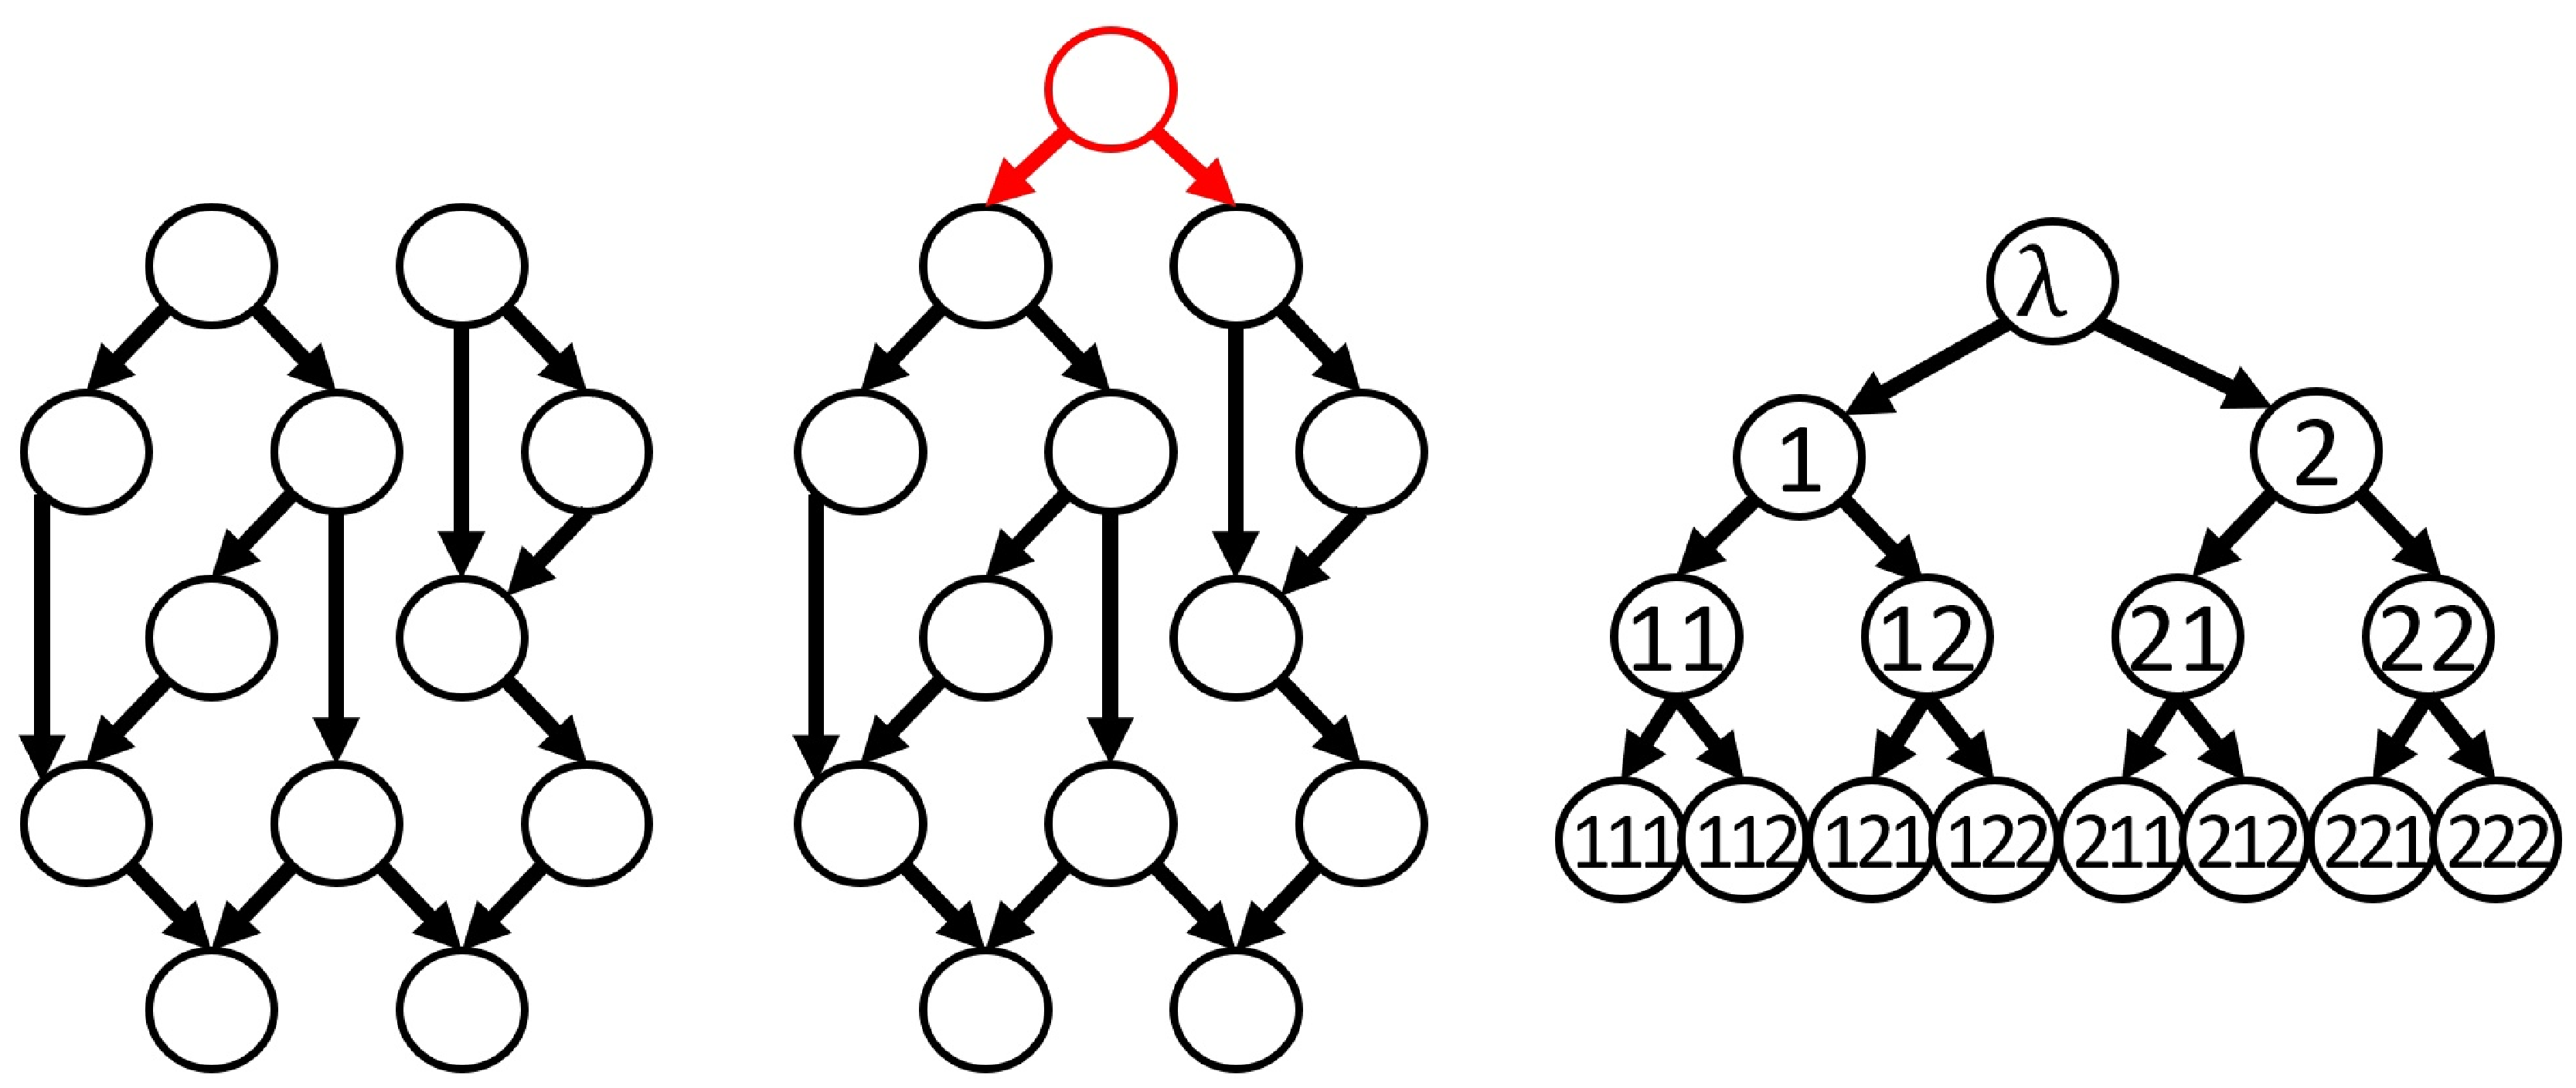
\includegraphics[width=\textwidth]{pic10.eps}
    \caption{given $H$ with $d=2, l=2$ (left) and $t=1$, the construction of $H'$ (center) and $M_{t, d, l}$ (right). $H'$ is obtained by adding a complete directed $d$-ary tree (red part) connected to each root of $H$. Moreover, the labeling of $M_{t, d, l}$ is constructed recursively by appending one character to the right of the parent's label.}
    \label{fig:10}
\end{figure}
}
\end{comment}



\begin{figure}[!t]
\begin{algorithm}[H]
	\caption{$\mathsf{GrowTokenTree}$}
	\label{growtokentree}
	\begin{algorithmic}[1]
    \WHILE{there is a vertex $u \in H'$ with token $T$ and a blue successor $v$ of $u$ whose all predecessors are placed token, and token $T$ has an \textit{untokened} child $T \cdot b$}
    \STATE place token $T \cdot b$ on $v$
    \ENDWHILE
    \RETURN \{$v \in V[H']$ | $v$ is placed a token\}
	\end{algorithmic}
\end{algorithm}
\end{figure}


\begin{figure}[!t]
\begin{algorithm}[H]
    \caption{$\mathsf{FindEmbedding}$}
	\label{findEmbedding}
	\begin{algorithmic}[1]
    \STATE place root token $\lambda$ on root of $H'$
    \STATE $i \leftarrow 1$
    \STATE $X_i  \leftarrow$ call $\mathsf{GrowTokenTree}$
    \WHILE{$|X_i| < |V[M_{t, d, l}]|$ and $H'$ has at least one blue vertex}
    \IF{there is a vertex $v \in H'$ with token $T$ such that $v$ has no blue successor and $T$ has at most one \textit{tokened} child}
    \STATE remove $T$ from $H'$
    \IF{$T$ had one \textit{tokened} child $T \cdot b$}
    \STATE replece all tokens $T \cdot b \cdot S$ with $T \cdot S$ on $H'$
    \ENDIF
    \ELSE
    \RETURN $X_i$
    \ENDIF
    \STATE $i \leftarrow i+1$
    \STATE $X_i \leftarrow$ call $\mathsf{GrowTokenTree}$
    \ENDWHILE
	\end{algorithmic}
\end{algorithm}
\end{figure}


\begin{comment}
\ifthenelse{\boolean{Draft}}{
\begin{figure}[t]
    \centering
    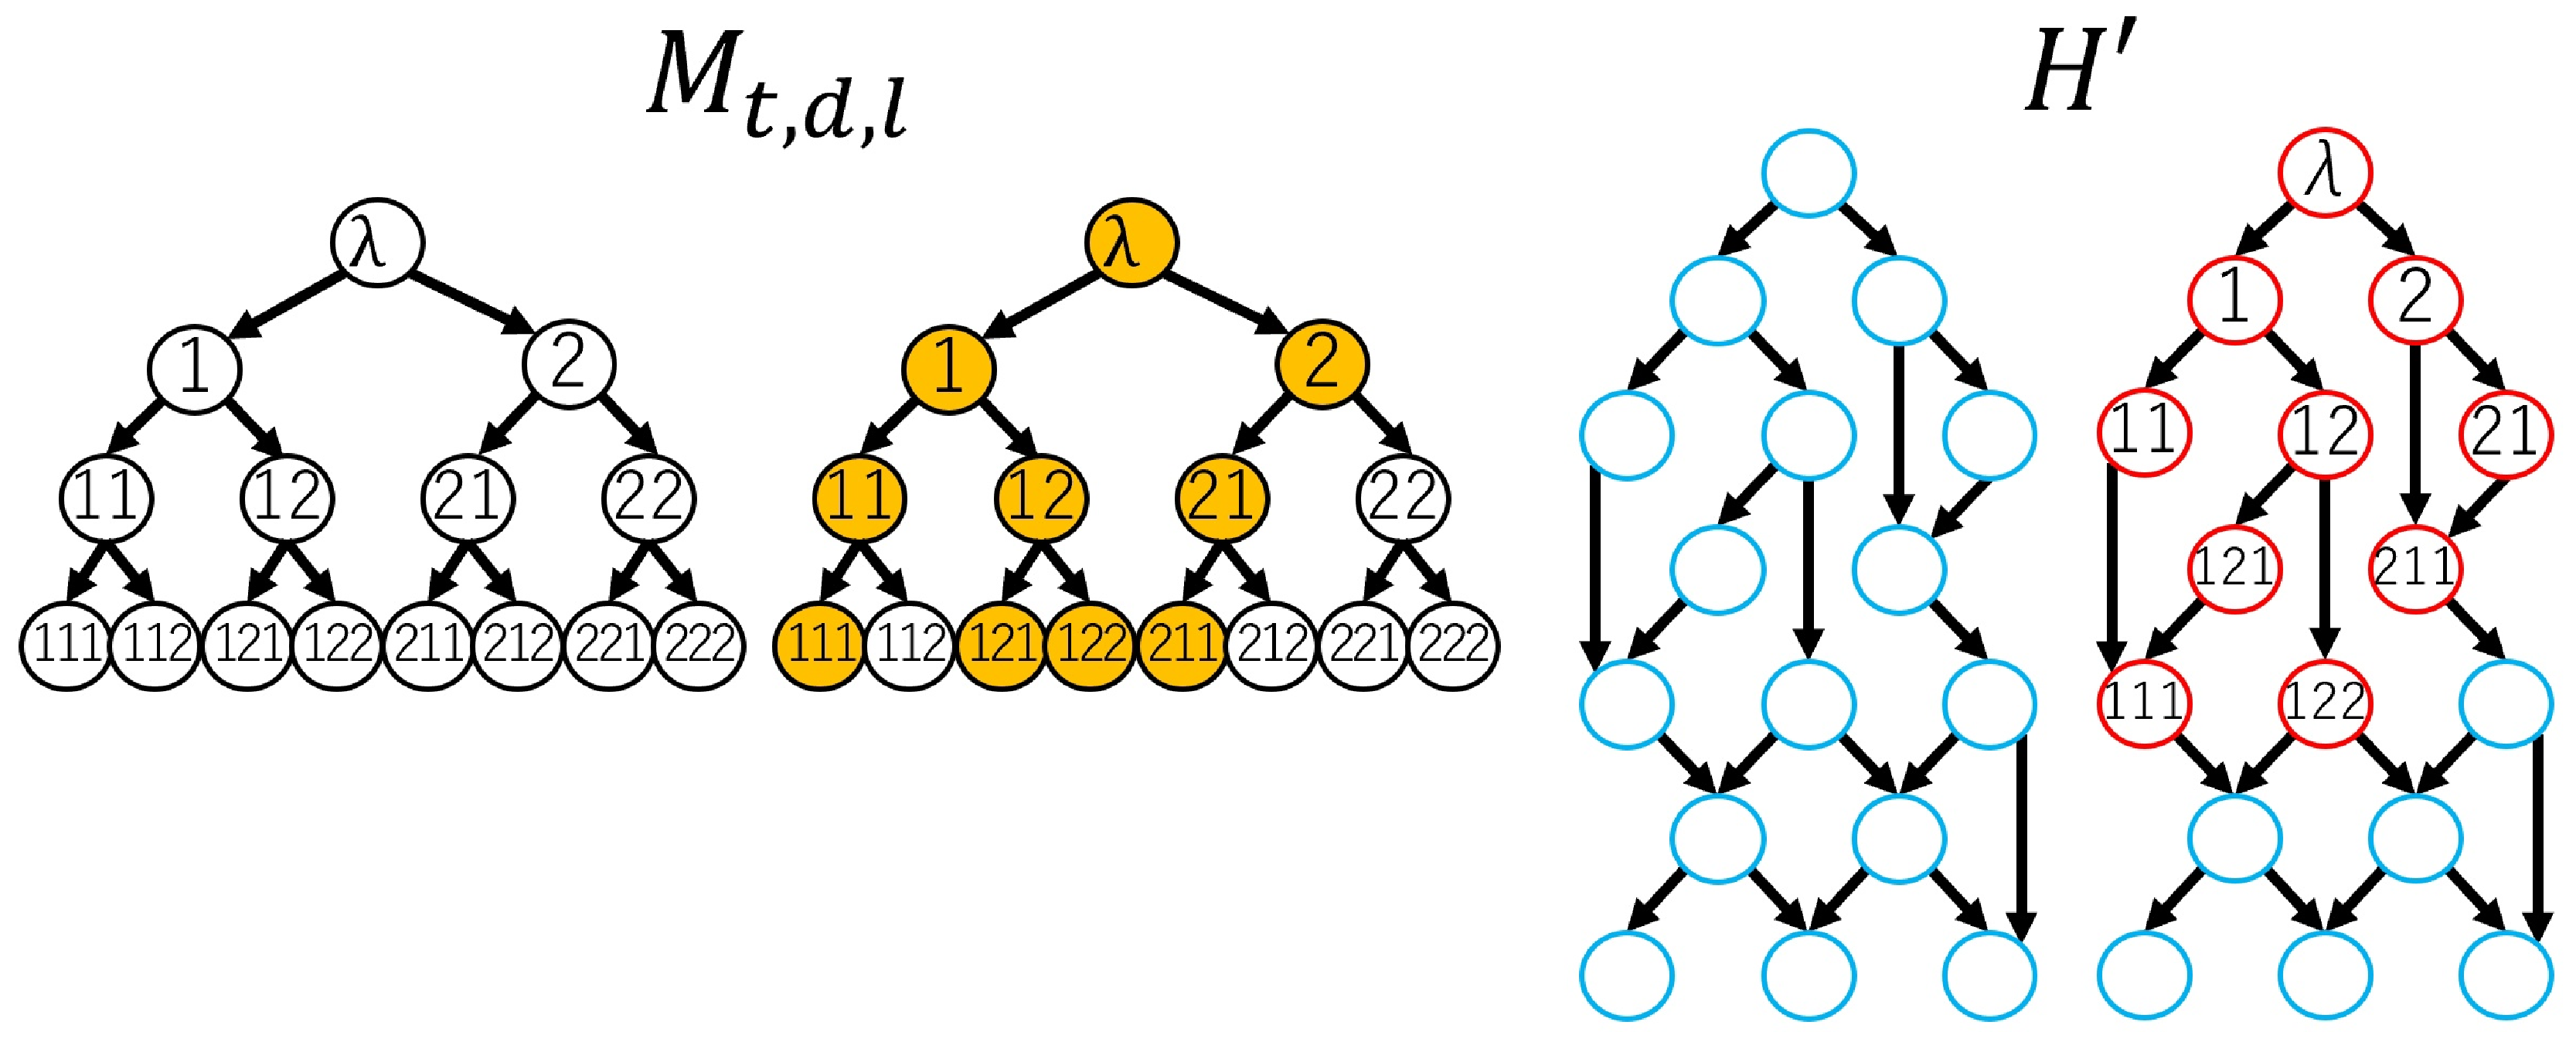
\includegraphics[width=\textwidth]{pic11.eps}
    \caption{Illustration of the operation of $\mathsf{GrowTokenTree}$. The orange tokens in $M_{t, d, l}$ indicate \textit{tokened} tokens. Starting from each left state and ending with each right state. $\mathsf{GrowTokenTree}$ places tokens of $M_{t, d, l}$ onto vertices of $H'$ while preserving the tree structure}
    \label{fig:11}
\end{figure}
}
\end{comment}



%$\mathsf{GrowTokenTree}$ and $\mathsf{FindEmbedding}$ are presented in Algorithms \ref{growtokentree} and \ref{findEmbedding}, respectively. $\mathsf{GrowTokenTree}$ (Algorithm \ref{growtokentree}) greedily places tokens of $M_{t, d, l}$ onto vertices of $H'$ while preserving the tree structure. A token can only be placed on a vertex whose predecessors already have tokens. This process continues until no more tokens can be placed, at which point the algorithm outputs the set of vertices in $H'$ placed tokens (see Figure~\ref{fig:11} in Appendix~\ref{location_figures}).

The algorithm consists of the main routine $\mathsf{FindEmbedding}$, presented in Algorithm~\ref{findEmbedding}, and the subroutine $\mathsf{GrowTokenTree}$, presented in Algorithm~\ref{growtokentree}, which is called from $\mathsf{FindEmbedding}$. $\mathsf{GrowTokenTree}$ greedily places tokens of $M_{t, d, l}$ onto vertices of $H'$ while preserving the condition of embeddings. A token can only be placed on a vertex whose all predecessors already have tokens. This process continues until no more tokens can be placed, at which point $\mathsf{GrowTokenTree}$ outputs the set of vertices in $H'$ on which tokens are placed (see Figure~\ref{fig:11} in Appendix~\ref{location_figures}).

\begin{comment}
\ifthenelse{\boolean{Draft}}{
\begin{figure}[t]
    \centering
    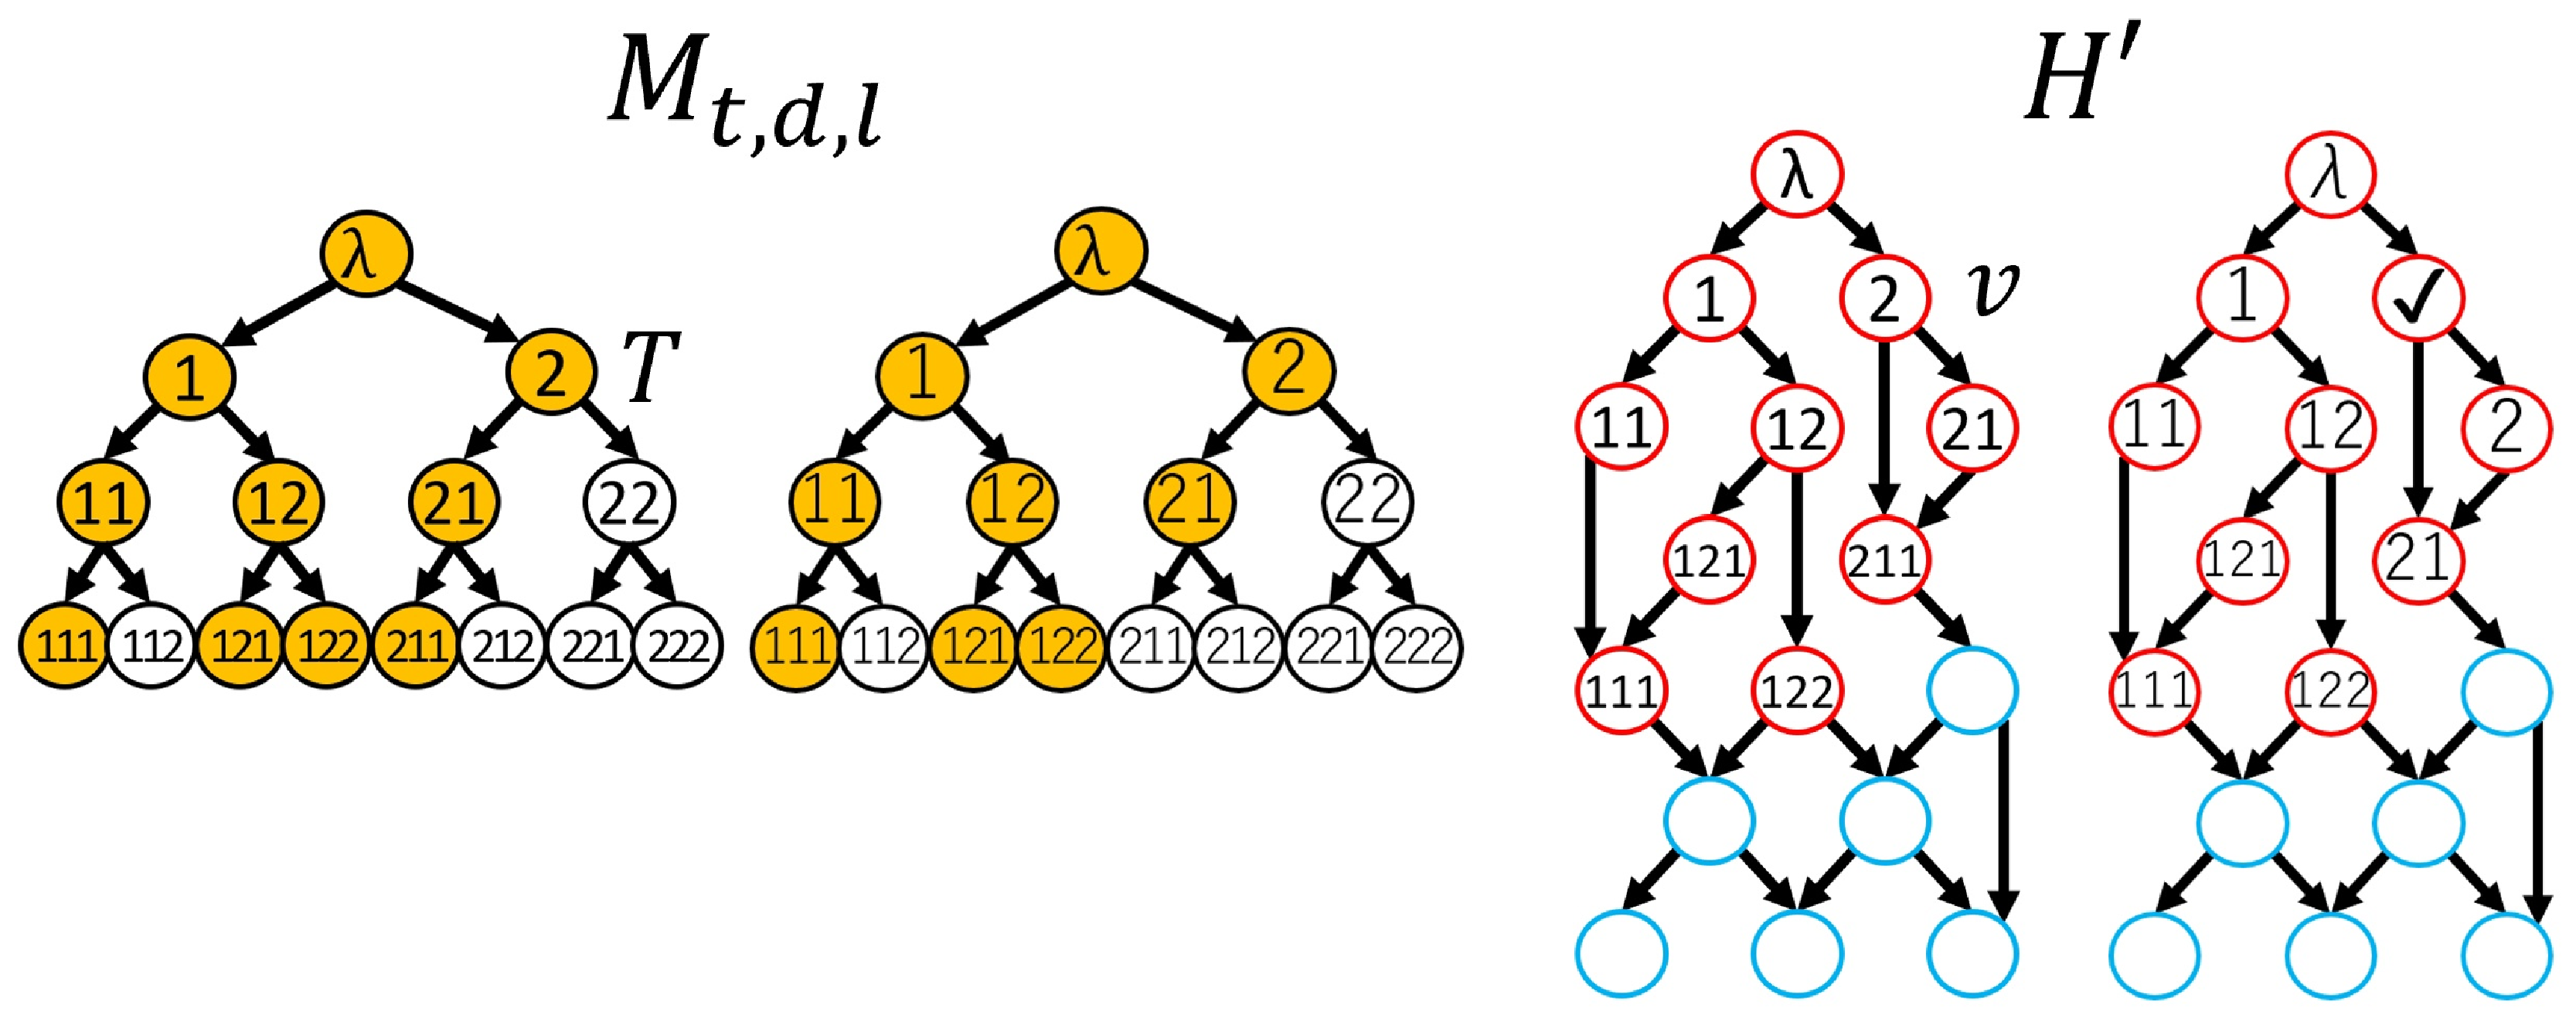
\includegraphics[width=\textwidth]{pic12.eps}
    \caption{Illustration of token replacement in $\mathsf{FindEmbedding}$. A vertex $v$ satisfying the condition in line 5 of the pseudocode (Algorithm \ref{findEmbedding}) and the token $T$ placed at $v$ are selected ($M_{t, d, l}$ left, $H'$ left), and $T$ is removed from $v$. Subsequently, $T$'s all \textit{tokened} descendants $T\cdot b \cdot S$ ($1 \leq b \leq d$ and $S$ is a string of arbitrary length) are replaced with $T \cdot S$ on $H'$.}
    \label{fig:12}
\end{figure}
}
\end{comment}


%$\mathsf{FindEmbedding}$ (Algorithm \ref{findEmbedding}) attempts to output a sequence of vertex sets $(X_1, X_2, \dots)$ that form a DAG-path-decomposition. Initially, a token $\lambda$ is placed on the single root of $H'$. Then, setting $i=1$, $\mathsf{GrowTokenTree}$ is executed, and the output is assigned to $X_1$. Subsequently, for each $i$, the following process is repeated. Assuming that $(X_1, X_2, \dots , X_i)$ has been constructed, if $X_i$ simultaneously uses all tokens of $M_{t, d, l}$, then it represents an embedding from $M_{t, d, l}$ to $H'$, which indicates the DAG-pathwidth of $H'$ is at least that of $M_{t, d, l}$. On the other hand, if all vertices of $H'$ have turned red, each vertex of $H'$ has had exactly one token placed on it. In this case, the sequence $(X_1, X_2, \dots, X_i)$ forms a DAG-path-decomposition of $H'$.

$\mathsf{FindEmbedding}$ attempts to output a sequence of vertex sets $(X_1, X_2, \dots)$ that form a DAG-path-decomposition. Initially, the algorithm places the token $\lambda$ on the single root of $H'$. The algorithm executes $\mathsf{GrowTokenTree}$ and assigns the output (set of vertices of $H'$) to $X_1$. Subsequently, for each $i = 1,2,\ldots$, the algorithm repeats the following procedure. Suppose that $(X_1, X_2, \dots , X_i)$ has been constructed. If $X_i$ includes all tokens of $M_{t, d, l}$, it represents an embedding from $M_{t, d, l}$ to $H'$, which indicates the DAG-pathwidth of $H'$ is at least that of $M_{t, d, l}$. Otherwise, if all vertices of $H'$ are red, we can show that the sequence $(X_1, X_2, \dots, X_i)$ forms a DAG-path-decomposition of $H'$ Otherwise (i.e., if not all tokens of $M_{t, d, l}$ are included in $X_i$ and at least one vertex in $H'$ remains blue), there may be potential for further execution of $\mathsf{GrowTokenTree}$ by modifying the token placement. Therefore, we consider removing the token $T$ placed on a vertex $v \in V[H']$ that satisfies the following two conditions:

\begin{enumerate}
    \item[(a)] All successor vertices of $v$ are red.
    \item[(b)] $T$ has at most one \textit{tokened} child token in $M_{t, d, l}$.
\end{enumerate}

Condition (a) corresponds to a forget operation in the DAG-path-decomposition, and condition (b) ensures that the embedding remains valid. A token $T$ can be removed from $v$ only if both conditions are met. In this process, removing $T$ might disconnect the \textit{tokened} token set in $M_{t, d, l}$. To maintain connectivity, all tokens in the directed tree rooted at the \textit{tokened} child $T \cdot b$ are relocated to the corresponding positions in the directed tree rooted at $T$. This replacement must proceed from the tokens closest to the root to those farther away to ensure that the replacement target tokens are always \textit{untokened}. This operation generates tokens that switch from \textit{tokened} to \textit{untokened}, allowing $\mathsf{GrowTokenTree}$ to be executed again, with its output denoted as $X_{i+1}$ (see Figure~\ref{fig:12} in Appendix~\ref{location_figures}). If no token satisfies both conditions (a) and (b), the algorithm returns the last output of $\mathsf{GrowTokenTree}$. This output represents evidence that the DAG-pathwidth of $H'$ is at least that of $M_{t, d, l}$.

This final process is the main difference from \cite{art8}. In \cite{art8}, there always exists a removable token $T$ until the algorithm terminates. In contrast, in this algorithm, there may be cases where such a token does not exist. This is because embedding of directed graphs is more difficult than that of undirected graphs, as it requires considering the directions of the edges.  


We first show the following lemma:

\begin{lemma}[proof in Appendix~\ref{appendix_D3}]\label{lemma_embedding}
    The subgraph $G'$ induced by the \textit{tokened} token set in $M_{t, d, l}$ is connected, and an embedding from $G'$ to $H'$ exists.
\end{lemma}




The algorithm $\mathsf{FindEmbedding}$ terminates when one of the following conditions is met: (1) in line 4, $H'$ no longer contains any blue vertices; (2) in line 4, $|X_i| = |V[M_{t, d, l}]|$ holds; or (3) the process in line 11 is executed. The following lemmas demonstrate that the algorithm functions correctly in each of these cases.

\begin{lemma}[proof in Appendix~\ref{appendix_D4}]\label{lemma_(1)}
    If $\mathsf{FindEmbedding}$ terminates under condition (1), then there exists a DAG-path-decomposition of $H$ with width at most $ld^{t+3}-1$.
\end{lemma}


\begin{lemma}[proof in Appendix~\ref{appendix_D5}]\label{lemma_(2)}
    If $\mathsf{FindEmbedding}$ terminates under condition (2), then $H$ can be splited into two disjoint subgraphs $A$ and $B$ such that $V[A] \cup V[B] = V[H]$ and $V[A] \cap V[B] = \varnothing$. Moreover, in $H$, only edges from $A$ to $B$ exist, and the DAG-pathwidth of $A$ is greater than $t$ but at most $ld^{t+3}-1$.
\end{lemma}



\begin{comment}
\ifthenelse{\boolean{Draft}}{
\begin{figure*}[t]
    \centering
    \begin{minipage}[c]{0.48\textwidth}
        \centering
        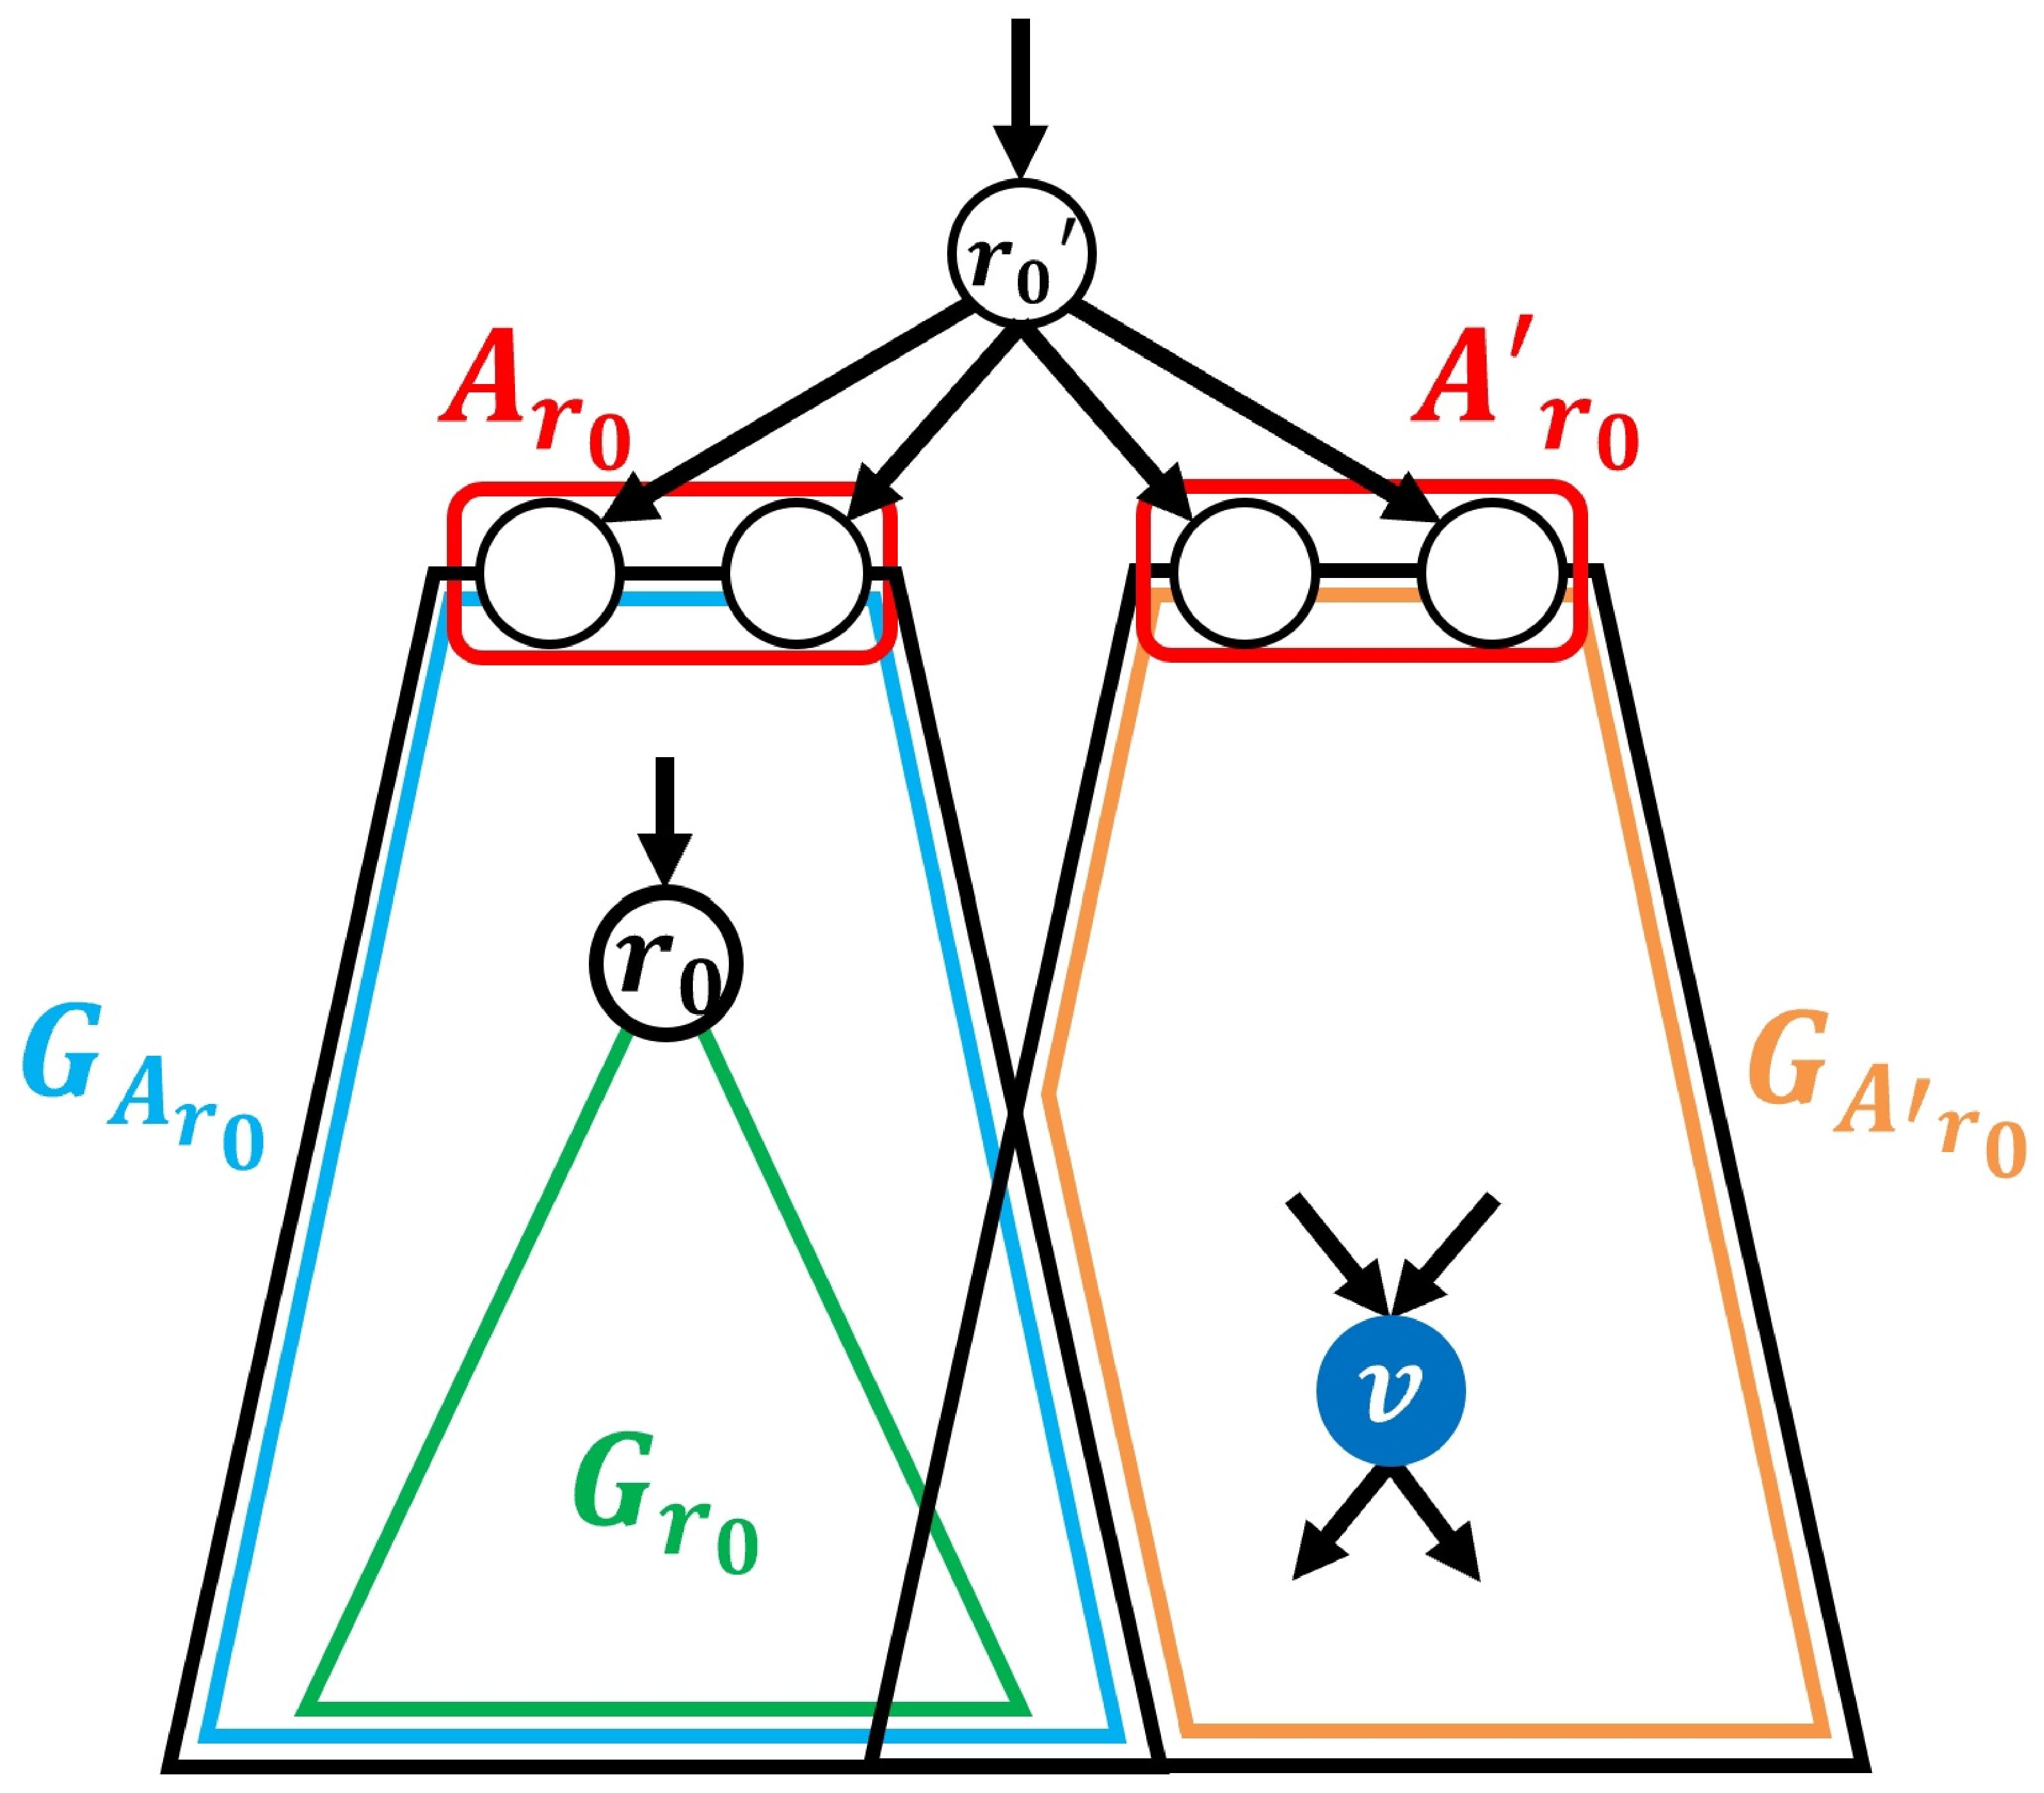
\includegraphics[width=6cm]{pic13.eps}
        \vspace{0.0cm}
        \caption{Illustration of the proof of \textbf{Lemma~\ref{blue_reachable}}. The recent common descendant of $r_0$ and $v$ is denoted as $r_0'$. The proof demonstrates that a contradiction arises if the blue vertex $v$ is not included in $G_{r_0}$, which consists of $r_0$ and its descendants.}
        \label{fig:13}
    \end{minipage}
    \hfill
    \begin{minipage}[c]{0.48\textwidth}
        \centering
        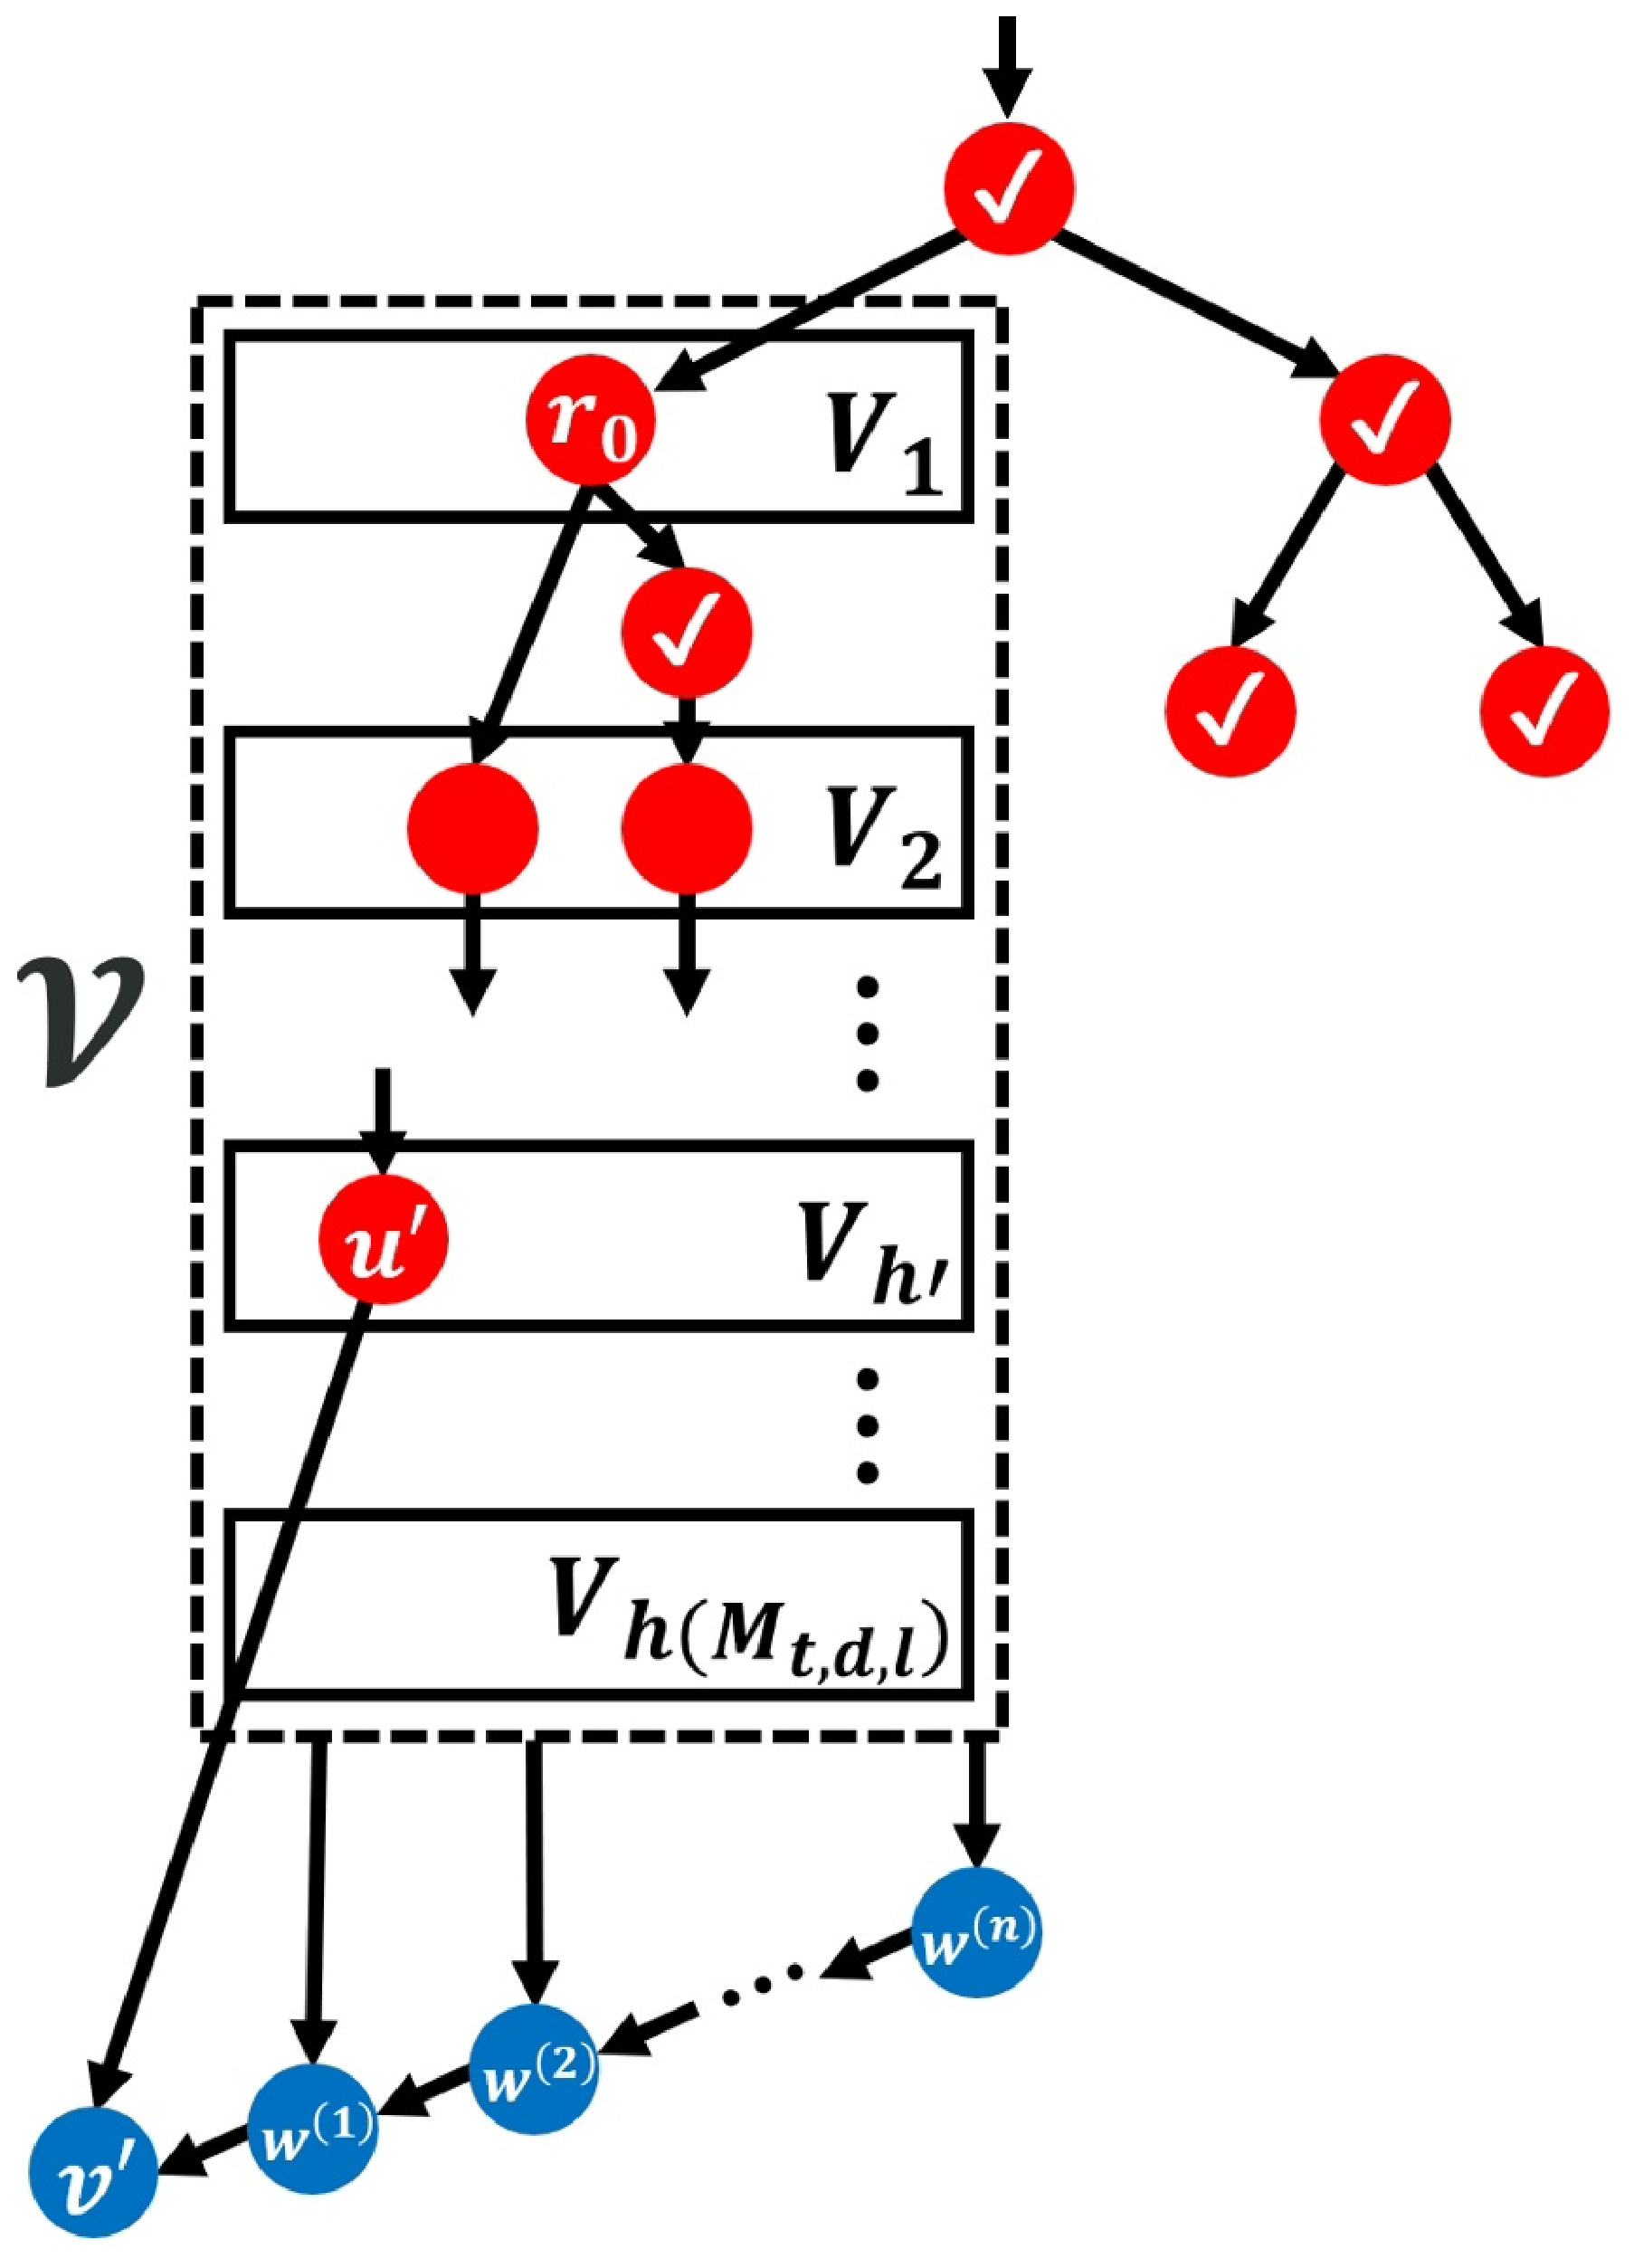
\includegraphics[width=6cm]{pic14.eps}
        \vspace{0.0cm}
        \caption{Illustration of the proof of \textbf{Lemma~\ref{lemma_(3)}}. The blue vertices represent blue, the red check-marked vertices indicate token-removed vertices, and the other red vertices indicate vertices with tokens placed on them. The proof demonstrates that a contradiction arises if there are no vertices in $V_{h(M_{t, d, l})}$.}
        \label{fig:14}
    \end{minipage}
\end{figure*}
}
\end{comment}



Before proving \textbf{Lemma~\ref{lemma_(3)}}, we show the following.  


\begin{lemma}[proof in Appendix~\ref{appendix_D6}]\label{blue_reachable}
    At any time $i = k$, let $r_0$ be the vertex of $H'$ on which the root token $\lambda$ is placed. Then, all blue vertices in $H'$ must have $r_0$ as an ancestor.
\end{lemma}


\begin{lemma}[proof in Appendix~\ref{appendix_D7}]\label{lemma_(3)}
    If $\mathsf{FindEmbedding}$ terminates at (3), then the DAG-pathwidth of $H$ is greater than $t$.
\end{lemma}

\textbf{Lemma~\ref{lemma_(1)}}, \textbf{\ref{lemma_(2)}}, and \textbf{\ref{lemma_(3)}} indicate \textbf{Theorem~\ref{approximation3}}. The proof is in appendix~\ref{appendix_D8}.

\begin{cor}[proof in Appendix~\ref{appendix_D9}]\label{cor}
    Given a DAG $H$ with $l$ roots and maximum outdegree $d$, and an integer $t$, there exists an $O(n^2)$ time algorithm that either provides evidence that the DAG-pathwidth of $H$ is greater than $t$, or provides a DAG-path-decomposition of width at most $O(ld^t)$.
\end{cor}








































\section{Conclusion}

In this study, we designed dynamic programming algorithms for solving various NP-hard problems on DAGs, using DAG-pathwidth as a parameter. Additionally, we demonstrated the existence of an $O(\log^{3/2} n)$-approximation algorithm for computing DAG-pathwidth, as well as a parameterized algorithm for constructing a DAG-path-decomposition with width $O(ld^k)$. The former is demonstrated by showing the equivalence between constructing DAG-path-decomposition and solving one-shot Black Pebbling game, while the latter leverages DAG embeddings. Notably, the latter algorithm is independent of the number of vertices in input graph and can also serve as an algorithm for estimating the one-shot Black Pebbling number.

A key challenge for future work is to further reduce the width $O(ld^k)$ of the parameterized algorithm. In particular, since the maximum outdegree $d$ may grow up to the vertex count $n$, we aim to explore methods to bound $d$ by a constant.
























\section*{Acknowledgements}

This work was supported by JSPS KAKENHI Grant Numbers JP24H00690 and JP24H00697.













%
% ---- Bibliography ----
%
% BibTeX users should specify bibliography style 'splncs04'.
% References will then be sorted and formatted in the correct style.
%
\nocite{*}
\bibliographystyle{splncs04}
\bibliography{mybibliography}
%



\appendix
\section{Proof of Chapter~\ref{chapter2}}

\subsection{The necessary and sufficient condition for the DAG-pathwidth 1}\label{appendix_A1}

\begin{definition}[directed caterpillar graph]
    A directed graph $G$ is said to be \textit{directed caterpillar graph} if it is a directed tree such that removing vertices with indegree 1 and outdegree 0 leaves a single directed path.
\end{definition}

\begin{lemma} \label{caterpillar}
    For a connected directed graph $G$ with $n$ vertices $(n > 2)$, the DAG-pathwidth of $G$ is 1 if and only if $G$ is directed caterpillar graph.
\end{lemma}


\begin{proof}
    If $G$ contains a directed cycle $C \subseteq V$, then noticing $|C| \geq 2$, $n > 2$ and $G$ is connected, there necessarily exists a vertex $v \in V[G]$ such that either $(u, v) \in E[V]$ with $u \in C$, or $(v, u) \in E[V]$ with $u \in C$. In this case, by the introduce rule of the nice DAG-path-decomposition, any DAG-path-decomposition of $G$ must contain a bag that includes $C \cup \{v\}$. Observing that $|C \cup \{v\}| \geq 3$, the DAG-pathwidth of $G$ must be at least 2. Consequently, if $G$ contains a cycle, its DAG-pathwidth is at least 2. Therefore, in the following, we consider the case where $G$ does not contain a cycle, that is, DAG.

    If there exists a vertex $v$ in $G$ with an in-degree of at least 2, then by (DPD2), any DAG-path-decomposition of $G$ must contain a bag that includes $v$ and all of its predecessor vertices. Thus, the DAG-path-width of $G$ is at least 2. Therefore, we consider only the case where $G$ has no vertex with in-degree 2 or greater, meaning that $G$ is a directed tree. First, we show that if $G$ is not directed caterpillar graph, then its DAG-path-width is at least 2. To do so, we consider cases based on the number of vertices in $G$. If $|V[G]| = 2$, then $G$ is clearly directed caterpillar graph. Similarly, when $|V[G]| = 3$ or $4$, $G$ is also directed caterpillar graph. The reason is as follows. Since $G$ is a directed tree, we select one of the longest paths in $G$ and denote its sequence of vertices as $P$. When $|V[G]| = 3$, then $|P| = 2$ or $|P| = 3$, both of which are clearly directed caterpillar graph. Similarly, when $|V[G]| = 4$, then $|P| = 2$, $|P| = 3$, or $|P| = 4$, all of which are also clearly directed caterpillar graph.
    
    Next, we consider the case where $G$ has at least 5 vertices. If $G$ is not directed caterpillar graph, then by definition, even after removing vertices of out-degree 0, $G$ still contains a branching. That is, there exists a vertex $v \in V[G]$ such that there are at least two vertex-disjoint paths of length 2 or greater starting from $v$. Let these paths be $P_1 = v, v_1, v_2, \dots$ and $P_2 = v, u_1, u_2, \dots$. By the rules of DAG-path-decomposition, any DAG-path-decomposition of $G$ must contain at least one bag that includes one of the following three vertex sets: $\{v, v_1, v_2\}$, $\{v, u_1, u_2\}$, or $\{v, v_1, u_1\}$. Therefore, the DAG-path-width is at least 2. Thus, by taking the contraposition, if DAG-path-width of $G$ is 1, then $G$ must be directed caterpillar graph by noting that the DAG-path-width is not smaller than 1 since $|V[G]| \geq 2$.
    
    Conversely, suppose $G$ is directed caterpillar graph. Each vertex $v$ in $G$ has leaf children $v_1, v_2, \dots, v_s$ with out-degree 0, and at most one non-leaf child with out-degree at least 1. If $v$ has no non-leaf child, we sequentially create bags $\{v, v_1\}, \{v, v_2\}, \dots, \{v, v_s\}$, thereby constructing a DAG-path-decomposition for $v$ and $\mathsf{suc}(v)$. If $v$ has a non-leaf child $u$, we sequentially create bags $\{v, v_1\}, \{v, v_2\}, \dots, \{v, v_s\}, \{v, u\}, \{u\}$, thus constructing a DAG-path-decomposition for $v$ and $\mathsf{suc}(v)$. Applying this process to all vertices, we obtain a DAG-path-decomposition of $G$ with width 1. Therefore, if $G$ is directed caterpillar graph, its DAG-path-width is 1.
\end{proof}






\section{Proofs of Chapter~\ref{chapter3}}

\subsection{\textbf{Lemma~\ref{DAG_path_decomposition(L(G))}}}\label{appendix_B1}
\begin{proof}
    Suppose that a nice DAG-path-decomposition $X=(X_1, X_2, \dots, X_s)$ of a DAG $G$ with width $w$ is given. For each $i=1, 2, \dots, s$, define $X^L_i = \{(u, v) \in E[G]~|~v \in X_i \}$. Then, $X^L=(X^L_1, X^L_2, \dots, X^L_s)$ forms a DAG-path-decomposition of $L(G)$ with width at most $w^2$. We prove this below. 
    
    First, $X^L$ satisfies (DPD1) for $L(G)$. Since the DAG-path-decomposition $X$ of $G$ ensures that each vertex appears in some bag by (DPD1), each edge of $G$ must also be contained in some bag $X^L_i$. 
    
    Furthermore, $X^L$ satisfies (DPD3) for $L(G)$. In $X$, (DPD3) ensures that the subgraph of $X$ induced by the bags containing any given vertex is a non-empty path. Similarly, in $X^L$, the subgraph induced by the bags containing any given edge of $G$ is also a non-empty path.
    
    Additionally, $X^L$ satisfies (DPD2) for $L(G)$. Consider a bag $X_k$ in $X$ that introduces a vertex $v$. By (DPD2) and (DPD3), for any vertex $u \in \mathsf{pred}(v)$, it holds that $u, v \in X_k$ and $v \notin X_{k-1}, u \in X_{k-1}$. Let $e_v$ be any edge with head $v$, and let $e_u$ be any predecessor of $e_v$ in $L(G)$. Since $e_u$ has head $u$, the edge $(e_u, e_v)$ in $L(G)$ satisfies $e_u, e_v \in X^L_i$ and $e_v \notin X^L_{i-1}$. Extending this argument to all $v$, we conclude that $X^L$ satisfies (DPD2) for $L(G)$. 
    
    Thus, $X^L$ is a DAG-path-decomposition of $L(G)$. Letting the width of $X^L$ be $w^L$, we note that the maximum in-degree $\delta_{in}$ of $G$ is at most $w$. Therefore, $w^L \leq \delta_{in} w \leq w^2$ holds. 

    Moreover, the complexity of constructing $X^L$ is $O(w^2n)$. This is because the number of bags in $X$ is $2|V[G]|+1$, and for each bag $X_i$, we only need to consider the predecessors of at most $w$ vertices it contains. Thus, the number of edges added to $X^L_i$ is at most $\delta_{in}w$. Consequently, the overall construction of $X^L$ takes $O(\delta_{in}wn) \leq O(w^2n)$ time.
\end{proof}




\subsection{\textbf{Lemma~\ref{mDEDS_mDiDS}}}\label{appendix_B2}
\begin{proof}
    First, we show that if $S$ is a DEDS of DAG $G$, then $S$ is also a DiDS of $L(G)$. If $S\in E[G]$ is a DEDS, for any edge $(v, w) \in E[G]$, either $(v, w) \in S$ holds or there exists some edge $(u, v) \in S$. In $L(G)$, for any vertex $(v, w) \in V[L(G)]$, either $(v, w) \in S$ holds or there exists some vertex $(u, v) \in S$. Thus, $S$ is a DiDS of $L(G)$. Similarly, if $S \in V[L(G)]$ is a DiDS of $L(G)$, then $S$ is a DEDS of $G$. Hence, the DEDS of $G$ and the DiDS of $L(G)$ correspond one-to-one. Therefore, the mDEDS of $G$ and the mDiDS of $L(G)$ are equal.
\end{proof}


\subsection{\textbf{Theorem~\ref{DEDS_FPT}}}\label{appendix_B3}
\begin{proof}
    By \textbf{Lemma~\ref{mDEDS_mDiDS}}, it suffices to compute the mDiDS of $L(G)$. By \textbf{Lemma~\ref{DAG_path_decomposition(L(G))}}, given a nice DAG-path-decomposition $X$ of $G$ with width $w$, we can construct a DAG-path-decomposition $X^L$ of $L(G)$ with width at most $w^2$ and convert to nice DAG-path-decomposition $X^L_{nice}$ in polynomial time. Therefore, we can compute the mDiDS of $L(G)$ using the algorithm described in \textbf{Theorem~\ref{theorem_dids}}. Noting that $X^L_{nice}$ has width $O(w^2)$ and $O(n^2)$ bags, the time complexity of this computation is $O(2^{w^2}w^2n^2)$.
\end{proof}



\subsection{Algorithm to solve DiDS problem and the proof of \textbf{Theorem~\ref{theorem_dids}}}\label{appendix_B4}
To construct an algorithm satisfying \textbf{Theorem~\ref{theorem_dids}}, we first define the function $\mathsf{DS}$. The function $\mathsf{DS}$ partitions each bag $X_i$ into two disjoint vertex sets $A_i, B_i \subseteq X_i ~(A_i \cup B_i = X_i, A_i \cap B_i = \varnothing)$. Then, among the directed dominating sets of the subgraph $G_i$ induced by $X_1 \cup X_2 \cup \dots \cup X_i$, it finds the smallest directed dominating set that includes all elements of $A_i$ and none of $B_i$. By computing this for all combinations of $A_i$ and $B_i$, we obtain the minimum dominating set for $G_i$. By considering all $i$, the minimum dominating set of the input graph $G$. The function $\mathsf{DS}$ is defined as follows:
    %
    \begin{equation}\label{def_ds}
        \mathsf{DS}(i, A_i, B_i) = \min \left\{ |S_i| \left |
        \begin{array}{l}
            S_i \subseteq X_1 \cup X_2 \cup  \dots \cup X_i, \\
            S_i \text{ is a DiDS of } G_i, \\
            A_i \subseteq S_i, B_i \cap S_i = \varnothing
        \end{array}
        \right. \right\}.
    \end{equation}
    

$\mathsf{DS}$ computes the size of the mDiDS of $G_i$. Below, we provide the recurrence formula for $\mathsf{DS}$, dividing cases based on whether $X_i$ introduces or forgets a vertex.

\begin{align*}
    \intertext{$\bullet$ When $X_i$ introduces $v \in V$:}
    &\mathsf{DS}(i, A_i, B_i) = 
    \begin{cases}
        \mathsf{DS}(i-1, A_i \backslash \{v\}, B_i) + 1 & (v \in A_i) \\
        \mathsf{DS}(i-1, A_i, B_i \backslash \{v\}) & (v \in B_i \text{ and } \mathsf{pred}(v) \cap A_i \neq \varnothing) \\
        \infty & (\text{otherwise})
    \end{cases}.
    \intertext{$\bullet$ When $X_i$ forgets $v \in V$:}
    &\mathsf{DS}(i, A_i, B_i) = \min \{\mathsf{DS}(i-1, A_i \cup \{v\}, B_i), \mathsf{DS}(i-1, A_i, B_i \cup \{v\})\}.
\end{align*}

Using $\mathsf{DS}$, we define the algorithm $\mathsf{Compute}(P)$, which outputs the size of the mDiDS of $G$ when given a nice DAG-path-decomposition $P$ of $G$.

\begin{enumerate}
    \item First Step: Set $\mathsf{DS}(0, \varnothing, \varnothing) = 0$.
    \item Execution Step: For each $X_i$ $(i=1, 2, ..., s)$ in $P$, compute $\mathsf{DS}(i, A_i, B_i)$ for all combinations of $A_i$ and $B_i$.
    \item Final Step: If $i = s$, output $\mathsf{DS}(s, \varnothing, \varnothing)$.
\end{enumerate}

To demonstrate \textbf{Theorem~\ref{theorem_dids}}, it is sufficient to prove the following two Lemmas.

\begin{lemma}\label{dids}
    $\mathsf{Compute}$ returns the size of the mDiDS of $G$.
\end{lemma}

\begin{proof}
    It suffices to show that for each $i$, $\mathsf{DS}(i, A_i, B_i)$ satisfies the definition (\ref{def_ds}) of $\mathsf{DS}$. We prove this by induction on $i$.
    
    Base Case ($i=0$): Clearly, definition (\ref{def_ds}) holds.
    
    Inductive Step ($i=k \rightarrow i=k+1$): Assume that $\mathsf{DS}(i, A_i, B_i)$ satisfies definition (\ref{def_ds}) for $i=k$. We consider cases where $X_{k+1}$ introduces or forgets $v \in V$.
    
    \begin{itemize}
        \item Case 1: $X_{k+1}$ introduces $v$
        
        If $v \in A_{k+1}$, then by (DPD2), $v$ does not dominate any vertex in $G_{k+1}$. Thus, $\mathsf{DS}(k+1, A_{k+1}, B_{k+1})$ is equal to $\mathsf{DS}(k, A_{k+1} \backslash \{v\}, B_{k+1}) + 1$. By induction, this satisfies definition (\ref{def_ds}).
        
        If $v \in B_{k+1}$ and $\mathsf{pred}(v) \cap A_{k+1} \neq \varnothing$, then some vertex $u \in A_{k+1}$ dominates $v$. Thus, $\mathsf{DS}(k+1, A_{k+1}, B_{k+1}) = \mathsf{DS}(k, A_{k+1}, B_{k+1} \backslash \{v\})$, which also satisfies definition (\ref{def_ds}) by induction.
        
        Otherwise, if $v \in B_{k+1}$ and $\mathsf{pred}(v) \cap A_{k+1} = \varnothing$, no vertex in $A_{k+1}$ dominates $v$. Hence, no valid mDiDS exists, and we set $\mathsf{DS}(k+1, A_{k+1}, B_{k+1}) = \infty$.
        
        \item Case 2: $X_{k+1}$ forgets $v$
        
        Since $G_{k+1} = G_k$, the mDiDS of $G_{k+1}$ is equal to the mDiDS of $G_k$. Thus, it is given by
        \begin{align*}
            \min \{\mathsf{DS}(k, A_{k+1} \cup \{v\}, B_{k+1}), \mathsf{DS}(k, A_{k+1}, B_{k+1} \cup \{v\})\},
        \end{align*}
        which satisfies definition (\ref{def_ds}).
    \end{itemize}
    Thus, by induction, \textbf{Lemma~\ref{dids}} is proven.
\end{proof}

\begin{lemma}
    Given a DAG $G$ with $n$ vertices and a DAG-path-decomposition $P$ of width $w$, $\mathsf{Compute}(P)$ runs in $O(2^w w n)$ time.
\end{lemma}

\begin{proof}
    Since $|X_i| \leq w+1$, the number of combinations of $A, B$ is at most $2^{w+1}$. The number of bags is $2|V|+1$. Checking $\mathsf{pred}(v) \cap A_i \neq \varnothing$ takes $O(w)$ time. Thus, the overall complexity is $O(2^w w n)$.
\end{proof}








\subsection{Algorithm to solve MaxLOB problem and the proof of \textbf{Theorem~\ref{theorem_lob}}}\label{appendix_B5}

The input graph is assumed to be a DAG with a single root $r$. In this case, there must exist a directed spanning tree with the maximum number of leaves in $G$. It is sufficient to prove the following lemma.

\begin{lemma}\label{lemma_spanning}
    For a connected DAG $G$, having exactly one root $r$ is both necessary and sufficient for $G$ to have a directed spanning tree.
\end{lemma}

\begin{proof}
    If there are two or more vertices with in-degree 0 in $G$, it is evident that no directed spanning tree can exist. Conversely, if there exists exactly one vertex $r$ with in-degree 0, we arrange the vertices of $G$ in a topological order starting with $r$, denoted as $r, v_1, v_2, \dots, v_{n-1}$. Since $G$ is a connected DAG, each vertex $v_i\ (i=1, 2, \dots, n-1)$ other than $r$ must have at least one parent in the set $\{r, v_1, v_2, \dots, v_{i-1}\}$. For each vertex $v_i$, there exists a path $P_i$ from $r$ to $v_i$. When considering the union of all such paths, if the result is a directed tree, then it is a directed spanning tree. If there is a cycle, we can remove it by replacing part of the paths with cycles. This can be done for all cycles, transforming the union of all paths into a directed tree, which will be a directed spanning tree.

    If \( G \) has two or more vertices with in-degree 0, it is clear that no directed spanning tree can exist. Conversely, if there is exactly one vertex \( r \) with in-degree 0, we can arrange the vertices of \( G \) in a topological order starting from \( r \), denoted as \( r, v_1, v_2, \dots, v_{n-1} \). Since \( G \) is a connected DAG, every vertex \( v_i \) (\( i = 1, 2, \dots, n-1 \)) other than \( r \) must have at least one parent in the set \( \{ r, v_1, v_2, \dots, v_{i-1} \} \). Therefore, for each vertex \( v_i \), there exists a path \( P_i \) from \( r \) to \( v_i \). Considering the union of all such paths, if the result forms a directed tree, it is a directed spanning tree. If a cycle appears, there exist two paths \( P_i \) and \( P_j \) (\( i \neq j \)) and each containing an internal path $P'_i$ and $P'_j$ (\( P'_i \) and \( P'_j \) are vertex-disjoint paths with the same starting and ending points), respectively. In this case, by replacing \( P'_i \) in \( P_i \) with \( P'_j \), the cycle formed by \( P'_i \) and \( P'_j \) can be removed. By performing this operation for all cycles, the union of all paths \( P_i \) can be transformed into a directed tree. This directed tree is a directed spanning tree.

\end{proof}

To construct an algorithm satisfying \textbf{Theorem~\ref{theorem_lob}}, we define the function $\mathsf{LOB}$. Let the nice DAG-path-decomposition of DAG $G = (V, E)$ be $P = (X_1, X_2, \dots, X_s)$. For each $i$ $(i=1, 2, \dots, s)$, let vertex sets $A_i, B_i \subseteq V$ satisfy $A_i \cup B_i = X_i$ and $A_i \cap B_i = \varnothing$. Let $G_i$ be the subgraph of $G$ induced by the vertex set $X_1 \cup X_2 \cup \dots \cup X_i$.
This algorithm finds all directed spanning trees of $G_i$ in which $A_i$ forms the leaf set and $B_i$ does not form the leaf set. By calculating this for all combinations of $A_i$ and $B_i$, the maximum number of leaves directed spanning tree for $G_i$ is obtained. By performing this calculation for all $i$, the maximum number of leaves directed spanning tree for the input graph $G$ is obtained. $\mathsf{LOB}$ is defined as follows, where the leaf set of a directed tree $T$ is denoted as $\mathsf{Leaf}(T)$:

\begin{equation}\label{def_lob}
    \mathsf{LOB}(i, A_i, B_i) = \max \left\{ |\mathsf{Leaf}(T_i)| \left |
    \begin{array}{l}
        T_i = (V[T_i], E[T_i]) \text{ is a directed spanning}\\ \text{tree of } G_i \text{ rooted at } r, \\
        V[T_i] = V[G_i], E[T_i] \subseteq E[G_i], \\
        A_i \subseteq \mathsf{Leaf}(T_i), B_i \subseteq V[T_i] \backslash \mathsf{Leaf}(T_i)
    \end{array}
    \right. \right\}.
\end{equation}


The function $\mathsf{LOB}$ computes the MaxLOB for $G_i$. Below, we provide the recurrence relation for $\mathsf{LOB}$, dividing the cases based on whether $X_i$ introduces or forgets a vertex.

\begin{align}
    \intertext{$\bullet$ When $X_i$ introduces $v \in V$:}
    &\mathsf{LOB}(i, A_i, B_i) = \notag
    \begin{cases}
        \mathsf{LOB}(i-1, A_i \backslash \{v\}, B_i) + 1 &(v \in A_i \text{ and } \mathsf{pred}(v) \cap B_i \neq \varnothing) \\
        \mathsf{LOB}(i-1, A_i, B_i \backslash \{v\}) &(v \in B_i \text{ and } \mathsf{pred}(v) \cap B_i \neq \varnothing) \\
        -\infty &(otherwise)
    \end{cases}.
    \intertext{$\bullet$ When $X_i$ forgets $v \in V$:}
    &\mathsf{LOB}(i, A_i, B_i) = \notag
    \max \{\mathsf{LOB}(i-1, A_i \cup \{v\}, B_i), \mathsf{LOB}(i-1, A_i, B_i \cup \{v\})\}.
\end{align}

Using $\mathsf{LOB}$, we define the algorithm $\mathsf{Compute}(P)$ to output the solution of MaxLOB for $G$ when given a nice DAG-path-decomposition $P$ of $G$.


\begin{enumerate}
    \item First Step: If $V_r = \{r\}$, output 1 as the solution. Otherwise, set $\mathsf{LOB}(1, \{r\}, \varnothing) = -\infty, \mathsf{LOB}(1, \varnothing, \{r\}) = 0$.
    \item Execution Step: For each $X_i$ $(i=1, 2, ..., s)$ in $P$, compute $\mathsf{LOB}(i, A_i, B_i)$ for all combinations of $A_i$ and $B_i$.
    \item Final Step: If $i = s$, output $\mathsf{LOB}(s, \varnothing, \varnothing)$.
\end{enumerate}

To demonstrate \textbf{Theorem~\ref{theorem_lob}}, it is sufficient to prove the following two Lemmas.

\begin{lemma}\label{lob}
    $\mathsf{Compute}$ outputs the solution of MaxLOB for $G$.
\end{lemma}

\begin{proof}
    From the First Step of $\mathsf{Compute}$, if $G$ consists only of root $r$, it outputs 1. It is the solution to MaxLOB. Next, consider the case where $G$ contains vertices other than $r$. The proof of \textbf{Lemma~\ref{lob}} follows by showing that $\mathsf{LOB}(i, A_i, B_i)$ satisfies the definition (\ref{def_lob}) of $\mathsf{LOB}$ for each $i$. This is done by induction on $i$. For convenience, we refer to non-leaf vertices of a tree as stems.\\
    When $i=1$, the First Step of $\mathsf{Compute}$ gives $\mathsf{LOB}(1, \{r\}, \varnothing) = -\infty$ and $\mathsf{LOB}(1, \varnothing, \{r\}) = 0$. Since $r$ cannot be a leaf, it clearly satisfies the definition (\ref{def_lob}).\\
    For $i=k$, assume that $\mathsf{LOB}(i, A_i, B_i)$ satisfies definition (\ref{def_lob}). We consider the cases where $X_{k+1}$ introduces or forgets $v \in V$.
    \begin{itemize}
        \item Case 1: $X_{k+1}$ introduces $v \in V$
        \\
        If $v \in A_{k+1}$, by (DPD2), $\mathsf{pred}(v) \subseteq (A_{k+1} \cup B_{k+1})$. Since $B_{k+1}$ represents the stems of the directed spanning tree, $v$ can only be considered a leaf if there exists a stem vertex $u \in \mathsf{pred}(v) \cap B_{k+1}$. By assumption, in $G_k$, we have $\mathsf{LOB}(k, A_{k+1} \setminus \{v\}, B_{k+1})$ as valid.
        
        If $v \in B_{k+1}$ and there exists an $u \in \mathsf{pred}(v) \cap A_{k+1}$, we can include $v$ in the leaf set. The definition of $\mathsf{LOB}$ holds in this case as well.

        Otherwise, if $v \in B_{k+1}$ and $\mathsf{pred}(v) \cap A_{k+1} = \varnothing$, no valid directed spanning tree exists with $v$ as a leaf, so $\mathsf{LOB}(k+1, A_{k+1}, B_{k+1}) = -\infty$.

        \item Case 2: When $X_{k+1}$ forgets $v \in V$
        \\
        Since $G_{k+1} = G_k$, the MaxLOB of $G_{k+1}$ equals the MaxLOB of $G_k$. Thus, we have the recurrence:
        \[
        \mathsf{LOB}(k+1, A_{k+1}, B_{k+1}) = \max \left\{ \mathsf{LOB}(k, A_{k+1} \cup \{v\}, B_{k+1}), \mathsf{LOB}(k, A_{k+1}, B_{k+1} \cup \{v\}) \right\},
        \]
        which satisfies the definition of $\mathsf{LOB}$.
    \end{itemize}
    Thus, by induction, \textbf{Lemma~\ref{lob}} is proven.
\end{proof}

\begin{lemma}\label{complexity_lob}
    Let $G$ be a DAG with $n$ vertices. Given the DAG-path-decomposition $P$ of $G$ with width $w$, the algorithm $\mathsf{Compute}(P)$ outputs the result in $O(2^w w n)$ time.
\end{lemma}
    
\begin{proof}
    The First Step and Final Step can each be computed in $O(1)$ time. We now analyze the time complexity for the Execution Step. For each $X_i$, note that $|X_i| \leq w+1$, so the number of combinations of $A$ and $B$ is at most $2^{w+1}$. Additionally, by \textbf{Proposition~\ref{number_of_bag}}, we have $0 \leq i \leq 2|V|+1$. Furthermore, since the computation of $\mathsf{pred}(v)$ takes $O(w)$ time, the time complexity of computing $\mathsf{LOB}(i, A_i, B_i)$ is $O(w)$ if $X_i$ introduces a vertex and $O(1)$ if $X_i$ forgets a vertex. Therefore, the overall time complexity of $\mathsf{Compute}$ is $O(w 2^w n)$.
\end{proof}












\subsection{Algorithm to Solve the Disjoint Path Problem and Proof of \textbf{Theorem~\ref{theorem_disjoint_path}}}\label{appendix_B6}

To construct an algorithm satisfying \textbf{Theorem~\ref{theorem_disjoint_path}}, we define the function $\mathsf{Cal}$. Let $X = (X_1, X_2, \dots, X_s)$ be a nice DAG-path-decomposition of a DAG $G = (V, E)$. For each $i$ $(i = 1, 2, \dots, s)$, let the vertex sets $A^1_i, A^2_i, \dots, A^k_i, B_i \subseteq V$ satisfy $A^1_i \cup A^2_i \cup \dots \cup A^k_i \cup B_i = X_i$, and assume that any two of $A^1_i, A^2_i, \dots, A^k_i, B_i$ have no common elements. Define $G_i$ as the subgraph of $G$ induced by the vertex set $X_1 \cup X_2 \cup \dots \cup X_i$, and set $\mathscr{A}_i = (A^1_i, A^2_i, \dots, A^k_i)$.

The function $\mathsf{Cal}$ determines whether each $A^m_i\ (m=1, 2, \dots, k)$ can be part of a vertex-disjoint path starting from $s_m$ for each $G_i$. Among such combinations of vertex-disjoint paths, it finds the one with the minimum total path length. By computing this for all possible combinations of $A^1_i, A^2_i, \dots, A^k_i, B_i$, we obtain the minimum total length of vertex-disjoint paths in $G_i$. Performing this calculation for all $i$ yields the minimum total length of vertex-disjoint paths in the input graph $G$. The function $\mathsf{Cal}$ is defined as follows:

\begin{equation}\label{def_cal}
    \mathsf{Cal}(i, \mathscr{A}_i, B_i) = \min \sum_{m=1}^k (|P^m_i| - 1).
\end{equation}

Here, the vertex sets $P^m_i$ $(i \leq m \leq k)$ satisfy $P^m_i \subseteq X_1 \cup X_2 \cup \dots \cup X_i$, forming a vertex-disjoint path starting from $s_m$. Moreover, for $m' \neq m$, we require that $A^m_i \subseteq P^m_i$, $A^{m'}_i \cap P^m_i = \varnothing$, and $B_i \cap P^m_i = \varnothing$. Thus, $\mathsf{Cal}$ calculates the minimum total length of $k$ vertex-disjoint paths starting from $s_m$ in $G_i$.

Next, we provide the recurrence formulas for computing $\mathsf{Cal}$. The computation is divided into cases based on whether each $X_i$ introduces or forgets a vertex. Let $S = \{s_1, s_2, \dots, s_k\}$ and $T = \{t_1, t_2, \dots, t_k\}$ be the sets of start and end vertices, respectively.

\begin{align}
    \intertext{$\bullet$ When $X_i$ introduces $v \in S$ ($v = s_m$):}
    &\mathsf{Cal}(i, \mathscr{A}_i, B_i) = \label{cal0}
    \begin{cases}
        0                                                   &(A^m_i = \{v\}) \\
        \infty                                              &(\text{otherwise})
    \end{cases}.
    \intertext{$\bullet$ When $X_i$ introduces $v \in T$ ($v = t_m$):}
    &\mathsf{Cal}(i, \mathscr{A}_i, B_i) = \label{cal1}
    \begin{cases}
        \mathsf{Cal}(i-1, \mathscr{A}^m_i, B_i)+1                    &(v \in A^m_i \text{ and there exists } w \in \mathsf{pred}(v) \cap A^m_i \\
        & \text{such that } \mathsf{suc}(w) \cap A^m_i = \{v\}) \\
        \infty                                              &(\text{otherwise})
    \end{cases}.
    \intertext{$\bullet$ When $X_i$ introduces $v \in V \backslash (S \cup T)$:}
    &\mathsf{Cal}(i, \mathscr{A}_i, B_i) = \label{cal2}
    \begin{cases}
        \mathsf{Cal}(i-1, \mathscr{A}^m_i, B_i)+1                    &(v \in A^m_i \text{ and there exists } w \in \mathsf{pred}(v) \cap A^m_i \\
        & \text{such that } \mathsf{suc}(w) \cap A^m_i = \{v\}) \\
        \mathsf{Cal}(i-1, \mathscr{A}^m_i, B_i \backslash \{v\})     &(v \in B_i) \\
        \infty                                              &(\text{otherwise})
    \end{cases}.
    \intertext{$\bullet$ When $X_i$ forgets $v \in V$:}
    &\mathsf{Cal}(i, \mathscr{A}_i, B_i) = \label{cal3}
    \min \{\min_{1 \leq m \leq k} \{\mathsf{Cal}(i-1, \mathscr{\overline{A}}^m_i, B_i)\}, \mathsf{Cal}(i-1, \mathscr{A}^m_i, B_i \cup \{v\})\}.
\end{align}

For any $v \in V$, define $\mathscr{A}^m_i$ and $\mathscr{\overline{A}}^m_i$ as follows:
\begin{align*}
    \mathscr{A}^m_i &= (A^1_i, A^2_i,  \dots, A^m_i \backslash \{v\}, \dots, A^k_i). \\
    \mathscr{\overline{A}}^m_i &= (A^1_i, A^2_i,  \dots, A^m_i \cup \{v\}, \dots, A^k_i).
\end{align*}

Using $\mathsf{Cal}$, we present the algorithm $\mathsf{Compute}(P)$ that outputs a solution to the Disjoint Path Problem for a given nice DAG-path-decomposition $P$ of DAG $G$.

\begin{enumerate}
    \item Preprocessing: If the input graph consists of a single vertex $s_1 = t_1$, output 0. Otherwise, remove all incoming edges to each vertex $t \in T$. Let $G$ be the resulting graph.
    \item First Step: Set $\mathsf{Cal}(0, (\varnothing, \varnothing, \dots, \varnothing), \varnothing) = 0$.
    \item Execution Step: For each $X_i$ $(i=1, 2, \dots, s)$ in $P$, compute $\mathsf{Cal}(i, \mathscr{A}_i, B_i)$ for all combinations of $\mathscr{A}_i, B_i$.
    \item Final Step: If $i = s$, output $\mathsf{Cal}(s, (\varnothing, \varnothing, \dots, \varnothing), \varnothing)$.
\end{enumerate}


To demonstrate \textbf{Theorem~\ref{theorem_disjoint_path}}, it is sufficient to prove the following two Lemmas.

\begin{lemma}\label{dpp}
    $\mathsf{Compute}$ outputs a solution to the Disjoint Path Problem of $G$.
\end{lemma}

\begin{proof}
    If the input graph $G$ consists of a single vertex $s_1 = t_1$, then $\mathsf{Compute}$ outputs 0 due to the preprocessing step. This is clearly a valid disjoint path of $G$. Now, suppose that $G$ consists of more than one vertex. When a bag $X_i$ introduces a vertex $v \in V$, $v$ is included in exactly one of $A^1_i, A^2_i, \dots, A^k_i, B_i$. By considering this property from 1 to $i$, we can establish that each path $P^m_i$ remains a vertex-disjoint path. Additionally, let $X_{i_s}$ be the bag introducing a starting vertex $s_m \in S$. Any vertex introduced at $X_{i'}$ $(i' < i_s)$ does not belong to the path $P^m_{i_s}$ because if a vertex $u$ is introduced at $X_{i'}$ and $A^m_{i'} = \{u\}$, then $\mathsf{pred}(u) \cap A^m_{i'} = \varnothing$. Consequently, due to condition~\ref{cal2}, $\mathsf{Cal}$ outputs $\infty$. Similarly, for an endpoint $t_m \in S$, let $X_{i_t}$ be the bag introducing it. Any vertex introduced at $X_{i'}$ $(i_t < i')$ does not belong to the path $P^m_{i'}$ because if a vertex $w$ is introduced at $X_j$ $(i_t < j)$ and $w \in \mathsf{suc}(t_m)$ in the original graph before preprocessing, then by the rule of DAG-path-decomposition, if $w \in A^m_j$, it must be that $t_m \in A^m_j$. If $\mathsf{pred}(w) \cap (A^m_j \setminus \{t_m\}) = \varnothing$, then by preprocessing, $\mathsf{pred}(w) \cap A^m_j = \varnothing$, making $\mathsf{Cal}$ return $\infty$ due to condition~\ref{cal2}. Otherwise, if there exists a vertex $p \in \mathsf{pred}(w) \cap A^m_j$ $(p \neq t_m)$, then there exists a vertex $q \in A^m_j$ $(p \in \mathsf{pred}(q) \cap (A^m_j \setminus \{w\})$ and $\mathsf{suc}(p) \cap (A^m_j \setminus \{w\}) = \{q\})$. Since preprocessing removes edge $(t_m, w)$, we find that $\{q, w\} \subseteq \mathsf{suc}(p) \cap A^m_j$, making $\mathsf{Cal}$ return $\infty$. Using the same argument, any vertex $w'$ introduced after $X_j$ and included in $A^m_l$ $(j < l)$ will result in $\mathsf{Cal}$ returning $\infty$. Thus, vertices introduced after $X_{i_t}$ do not get added to the path $P^m_{i_t}$. 

    With the above observations, it suffices to prove that for each $i$ $(i_s \leq i \leq i_t)$, there exists some $m$ $(1 \leq m \leq k)$ such that $\mathsf{Cal}(i, \mathscr{A}_i, B_i)$ satisfies the definition~(\ref{def_cal}). We prove this by induction on $i$. 

    Base Case: When $i = i_s$, equation~\ref{cal0} ensures that if $A^m_{i_s} = \{s_m\}$, then $\mathsf{Cal}(i_s, \mathscr{A}_{i_s}, B_{i_s}) = 0$, indicating that the path $P^m_{i_s}$ consists only of $s_m$ with length 0, which clearly satisfies definition~(\ref{def_cal}). If $A^m_{i_s} \neq \{s_m\}$, then $\mathsf{Cal}$ outputs $\infty$, implying that no path starting at $s_m$ is constructed, which also satisfies definition~(\ref{def_cal}).

    Inductive Step: Assume that for some $i$ $(i_s \leq i < i_t)$, $\mathsf{Cal}(i, \mathscr{A}_i, B_i)$ satisfies definition~(\ref{def_cal}). We consider two cases based on whether $X_{i+1}$ introduces or forgets a vertex.

    \begin{itemize}
        \item Case 1: $X_{i+1}$ introduces $v \in V$
        \\
        If $v \in A^m_{i+1}$, let $u$ be the last introduced vertex in $A^m_{i+1}$ before $v$. By (DPD2), an edge $(u, v)$ must exist, or an edge $(u', v)$ exists for some $u' \in A^m_{i+1}$. If $(u, v)$ exists, equation~\ref{cal2} ensures that $\mathsf{Cal}(i+1, \mathscr{A}_{i+1}, B_{i+1}) = \mathsf{Cal}(i, \mathscr{A}^m_{i+1}, B_{i+1}) + 1$. By assumption, $\mathsf{Cal}(i, \mathscr{A}^m_{i+1}, B_{i+1})$ represents the minimal total path length when $m$-th path extends from $s_m$ to $u$. Since adding $v$ to the path increases length by 1, $\mathsf{Cal}(i+1, \mathscr{A}_{i+1}, B_{i+1})$ maintains the minimum path sum and satisfies definition~(\ref{def_cal}).
    
        If $v \in B_{i+1}$, since $v \notin A^m_{i+1}$, the total minimum path length remains $\mathsf{Cal}(i, \mathscr{A}^m_{i+1}, B_{i+1} \setminus \{v\})$, which satisfies definition~(\ref{def_cal}).
        
        \item Case 2: $X_{i+1}$ forgets $v \in V$
        \\
        Since $G_{i+1} = G_i$, the total path length remains unchanged. Thus, the two cases—whether $v$ is part of some path or in $B_i$—are considered. Taking the minimum of both values from the previous step, equation~\ref{cal3} correctly determines the minimum path sum, satisfying definition~(\ref{def_cal}).
    \end{itemize}
    By induction, \textbf{Lemma~\ref{dpp}} is proven.
\end{proof}


\begin{lemma}
    Let the number of vertices in the DAG $G$ be $n$. Given a DAG-path-decomposition $P$ of $G$ with width $w$, the function $\mathsf{Compute}(P)$ computes the result in $O((k+1)^w(w^2+k)n+n^2)$ time, where $k$ is the size of the terminal set.
\end{lemma}

\begin{proof}
    In preprocessing, it can be determined in $O(1)$ time whether $G$ consists of a single vertex. Also, removing all edges entering each $t \in T$ takes $O(n^2)$ time. The First Step and Final Step can each be computed in $O(1)$ time. Below, we analyze the time complexity of the Execution Step. For each $X_i$, notice that $|X_i| \leq w+1$. The number of combinations of $A^1_i, A^2_i, \dots, A^k_i, B_i$ is at most $(k+1)^{w+1}$. Furthermore, by \textbf{Proposition~\ref{number_of_bag}}, we know that $0 \leq i \leq 2|V|+1$. Additionally, since the calculation of $\mathsf{pred}(v)$ and $\mathsf{suc}(v)$ takes $O(w)$ time, the time complexity of $\mathsf{Cal}(i, \mathscr{A}_i, B_i)$ is $O(w^2)$ when $X_i$ is an "introduce" operation, and $O(k)$ when it is a "forget" operation. Therefore, the total time complexity of $\mathsf{Compute}$ is $O((k+1)^w(w^2+k)n+n^2)$.
\end{proof}

By modifying the above algorithm, we can construct algorithms for solving related problems, such as the edge-disjoint path problem.






\subsection{Algorithm to Solve the DST Problem and the Proof of \textbf{Theorem~\ref{theorem_DST}}}\label{appendix_B7}

To construct an algorithm satisfying \textbf{Theorem~\ref{theorem_DST}}, we define the function $\mathsf{ST}$. Let the nice DAG-path-decomposition of the DAG $G = (V, E)$ be $P = (X_1, X_2, \dots, X_s)$. For some $i$ $(i = 1, 2, \dots, s)$, let $A_i, B_i \subseteq V$ satisfy $A_i \cup B_i = X_i$ and $A_i \cap B_i = \varnothing$. Let $G_i$ be the subgraph of $G$ induced by the vertex set $X_1 \cup X_2 \cup \dots \cup X_i$.

The function $\mathsf{ST}$ computes the directed Steiner tree that includes all vertices in $R \cap V[G_i]$ for each $G_i$. The Steiner tree contains all vertices in $A_i$, excludes all vertices in $B_i$, and has the minimum size. By computing this for all combinations of $A_i$ and $B_i$, we obtain the minimum directed Steiner tree for $G_i$. By repeating this computation for all $i$, we eventually obtain the minimum directed Steiner tree for the entire input graph $G$. Let the weight of edge $e$ be denoted by $d(e)$. We define the function $\mathsf{ST}$ as follows:

\begin{equation}
    \mathsf{ST}(i; A_i, B_i) = \min \left\{ \sum_{(u, v) \in E[G_{T_i}]} d(u, v) \mid
    \begin{array}{l} \label{ST_def}
        T_i \subseteq X_1 \cup X_2 \cup \dots \cup X_i \\
        G_{T_i} \text{ is a directed tree with root } r \\ \text{ on } G_i \\
        V[G_{T_i}] = T_i,  E[G_{T_i}] \subseteq E[G_i] \\
        A_i \subseteq T_i, B_i \cap T_i = \varnothing \\
        \forall t \in R \cap G_i, t \in T_i
    \end{array}
    \right\}.
\end{equation}

For each $i$, if a directed tree $G_{T_i}$ exists that satisfies the above conditions, we call it the optimal directed Steiner tree and denote it by $G^{opt}_{T(i, A_i, B_i)}$. The tree $G^{opt}_{T(s, \varnothing, \varnothing)}$ is the minimum directed Steiner tree (minimum-DST).

The following provides the computation formula for $\mathsf{ST}$. We compute it by distinguishing between the cases when $X_i$ introduces or forgets a vertex. Note that since the input graph is a DAG, any strongly connected component introduced in a nice DAG-path-decomposition consists of only a single vertex.

\begin{align}
    \intertext{$\bullet$ When $X_i$ introduces a vertex $v \in V$}
    &\mathsf{ST}(i; A_i, B_i) = \label{ST_intro}
    \begin{cases}
        \mathsf{ST}(i-1; A_i \setminus \{v\}, B_i) + \underset{w \in \mathsf{pred}(v) \cap A_i}{\min} d(w, v) & (\text{if } v \in A_i \text{ and } \\ &\mathsf{pred}(v) \cap A_i \neq \varnothing) \\
        \mathsf{ST}(i-1; A_i, B_i \setminus \{v\}) & (\text{if } v \in B_i \text{ and } \\ &v \notin R \cup \{r\}) \\
        \infty & (\text{otherwise})
    \end{cases}.
    \intertext{$\bullet$ When $X_i$ forgets a vertex $v \in V$}
    &\mathsf{ST}(i; A_i, B_i) = \min \left\{ \mathsf{ST}(i-1; A_i \cup \{v\}, B_i), \mathsf{ST}(i-1; A_i, B_i \cup \{v\}) \right\}. \label{ST_forget}
\end{align}

When given a nice DAG-path-decomposition $P$ of DAG $G$, root $r$, and terminal set $R$, the following algorithm $\mathsf{Compute}(P)$ outputs the total weight of the minimum-DST of $G$ that contains all vertices in $R$:

\begin{enumerate}
    \item Preprocessing: Let $V_r$ be the set of vertices reachable from the root $r$ in $G$. For each bag $X_i$ of $P$, remove any vertex $v \in V \backslash V_r$ from $X_i$. The resulting sequence of vertex sets is converted back into a nice DAG-path-decomposition, which we denote as $P' = (X_1, X_2, \dots , X_{s'})$ for convenience.
    \item First Step: Set $\mathsf{ST}(1; \{r\}, \varnothing) = 0$.
    \item Execution Step: For each $X_i$ $(i=2, 3, \dots, s')$, compute $\mathsf{ST}(i; A_i, B_i)$ for all combinations of $A_i$ and $B_i$.
    \item Final Step: If $i = s'$, output $\mathsf{ST}(s'; \varnothing, \varnothing)$.
\end{enumerate}

To demonstrate \textbf{Theorem~\ref{theorem_DST}}, it is sufficient to prove the following two lemmas.

\begin{lemma}\label{dst}
    The function $\mathsf{Compute}$ outputs the total weight of the minimum-DST of $G$, with root $r$ and containing all vertices in $R$.
\end{lemma}

\begin{proof}
    First, we show that the solution remains unchanged after preprocessing. Since $V_r$ is the set of vertices reachable from the root $r$, any $v \in V \backslash V_r$ will not be included in the desired minimum-DST. Therefore, even if we consider the graph $G' = G[V \backslash V_r]$, the solution does not change. Moreover, $P'$ is a nice DAG-path-decomposition of $G'$, and using $P'$ as input to $\mathsf{ST}$ will yield the same result. Additionally, the width of $P'$ does not exceed that of $P$.

    Next, we show that after preprocessing, $\mathsf{Compute}$ outputs the minimum-DST of $G$ that contains all vertices in $R$. This can be shown by demonstrating that equations (\ref{ST_intro}) and (\ref{ST_forget}) correspond to definition (\ref{ST_def}) for each $i$, which we prove by mathematical induction on $i$.
    
    When $i=1$, clearly $\mathsf{ST}(1; \{r\}, \varnothing) = 0$ satisfies definition (\ref{ST_def}).
    
    Assume that for $i=k$ $(1 \leq k < s')$, equations (\ref{ST_intro}) and (\ref{ST_forget}) satisfy definition (\ref{ST_def}). We will now show that for $i=k+1$, equations (\ref{ST_intro}) and (\ref{ST_forget}) hold definition (\ref{ST_def}) as well.

    \begin{itemize}
    \item Case 1: $X_{k+1}$ introduces $v$\\
    We consider the case where $v \in A_{k+1}$ and $v \in B_{k+1}$ separately. 
    When $v \in A_{k+1}$, if $\mathsf{pred}(v) \cap A_{k+1} = \varnothing$, then there are no predecessors of $v$ in $A_i$. In this case, by (DPD2), since no predecessors of $v$ are introduced after $X_{k+1}$, the directed tree containing $v$ has $v$ as one of its roots. Since this tree cannot have $r$ as its only root, we set $\mathsf{ST}(k+1; A_{k+1}, B_{k+1}) = \infty$ to indicate that the directed tree $G^{opt}_{T(k, A_{k+1}, B_{k+1})}$ represented by equation (\ref{ST_def}) does not exist. On the other hand, if $\mathsf{pred}(v) \cap A_{k+1} \neq \varnothing$, then there exists at least one predecessor $w \in A_{k+1} \backslash \{v\}$ of $v$. If a directed tree $G^{opt}_{T(k, A_{k+1} \backslash \{v\}, B_{k+1})}$ exists, then $w \in G^{opt}_{T(k, A_{k+1} \backslash \{v\}, B_{k+1})}$. By the preprocessing operation, $w$ is reachable from $r$. Therefore, $v$ is also reachable from $r$ through $w$, and $G^{opt}_{T(k, A_{k+1} \backslash \{v\}, B_{k+1}) \cup \{v\}}$ is a directed tree with $r$ as its root. The minimal total weight at that point is equal to $ \sum_{(u, v) \in E[G^{opt}_{T(k, A_{k+1} \backslash \{v\}, B_{k+1})}]} d(u, v) + \min_{w \in \mathsf{pred}(v) \cap A_i} d(w, v)$. By assumption, $\mathsf{ST}(k; A_k, B_k) = \sum_{(u, v) \in E[G^{opt}_{T(k, A_k, B_k)}]} d(u, v)$, and since $A_{k+1} \backslash \{v\} = A_k$ and $B_{k+1} = B_k$, we conclude that $\mathsf{ST}(k+1; A_{k+1}, B_{k+1})$ is represented by equation (\ref{ST_def}).

    Next, consider the case where $v \in B_{k+1}$. When $v \in R \cup \{r\}$, $\mathsf{ST}(k+1; A_{k+1}, B_{k+1}) = \infty$, indicating that no directed tree $G^{opt}_{T(k, A_{k+1}, B_{k+1})}$ exists as represented by equation (\ref{ST_def}). If $v \notin R \cup \{r\}$, then by equation (\ref{ST_def}), $v$ does not belong to the directed tree that is the solution. In this case, we have $G^{opt}_{T(k+1, A_{k+1}, B_{k+1} \backslash \{v\})} = G^{opt}_{T(k, A_k, B_k)}$. By assumption, $\mathsf{ST}(k; A_k, B_k) = \sum_{(u, v) \in E[G^{opt}_{T(k, A_k, B_k)}]} d(u, v)$, and since $A_{k+1} = A_k$ and $B_{k+1} \backslash \{v\} = B_k$, we conclude that $\mathsf{ST}(k+1; A_{k+1}, B_{k+1})$ is represented by equation (\ref{ST_def}).

    \item Case 2: $X_{k+1}$ forgets $v$\\
    From $G_{k+1} = G_k$, the directed tree $G^{opt}_{T(k+1, A_{k+1}, B_{k+1})}$ is equal to either $G_{T_A} = G^{opt}_{T(k, A_k, B_k)}$ when $v \in A_k$, or $G_{T_B} = G^{opt}_{T(k, A_k, B_k)}$ when $v \in B_k$, whichever has the smaller total weight. By assumption, if $v \in A_k$, then $\mathsf{ST}(k; A_k, B_k) = \sum_{(u, v) \in E[G^{opt}_{T_A}]} d(u, v)$, and if $v \in B_k$, then $\mathsf{ST}(k; A_k, B_k) = \sum_{(u, v) \in E[G^{opt}_{T_B}]} d(u, v)$. Furthermore, if $v \in A_k$, then $A_{k+1} \cup \{v\} = A_k$ and $B_{k+1} = B_k$; if $v \in B_k$, then $A_{k+1} = A_k$ and $B_{k+1} \cup \{v\} = B_k$. Therefore, we conclude that $\mathsf{ST}(k+1; A_{k+1}, B_{k+1})$ is represented by equation (\ref{ST_def}).
\end{itemize}
Thus, for $i = k+1$, both equations (\ref{ST_intro}) and (\ref{ST_forget}) represent equation (\ref{ST_def}). By mathematical induction, \textbf{Lemma~\ref{dst}} is proven.

\end{proof}


\begin{lemma}
    Let the number of vertices in the DAG $G = (V, E)$ be $n$. Given a DAG-path-decomposition $P$ of $G$ with width $w$, root $r \in V$, and terminal set $R \subseteq V$, where $k = |R|$, the function $\mathsf{Compute}(P, r, R)$ computes the optimal solution in $O(2^w(k+w)n + n^2)$ time.
\end{lemma}

\begin{proof}
    In preprocessing, the calculation of the set of vertices reachable from $r$ takes $O(n^2)$ time. The First Step and Final Step can each be computed in $O(1)$ time. Now, let’s analyze the time complexity of the Execution Step. For each $X_i$, notice that $|X_i| \leq w + 1$, so the number of combinations of $A_i$ and $B_i$ is at most $2^{w+1}$. Also, by \textbf{Proposition~\ref{number_of_bag}}, $0 \leq i \leq 2|V|+1$. Additionally, when introducing a vertex $v \in V$ in $X_i$, the computation of $\mathsf{pred}(v) \cap A_i \neq \varnothing$ and $\min$, as well as the check for $v \in R \cup \{r\}$, each takes $O(w)$, $O(w)$, and $O(k)$ time, respectively. Therefore, if $X_i$ introduces a vertex, the time complexity of calculating $\mathsf{ST}(i; A_i, B_i)$ is $O(k+w)$, and if $X_i$ forgets a vertex, the time complexity is $O(1)$. Hence, the time complexity of the Execution Step is $O(2^w(k+w)n)$. Thus, the overall time complexity of $\mathsf{Compute}$ is $O(2^w(k+w)n + n^2)$.
\end{proof}

Furthermore, by a simple extension of the above algorithm, we can efficiently solve the vertex-weighted directed Steiner tree problem.

\begin{theorem}
    Given a vertex-weighted DAG $G$ with terminal size $k = |R|$ and a nice DAG-path-decomposition of $G$ with width $w$, there exists an FPT algorithm that solves the vertex-weighted DST problem for $G$ in $O(2^w(k+w)n + n^2)$ time.
\end{theorem}





























\section{Proof of Chapter~\ref{chapter4}}

\subsection{\textbf{Lemma~\ref{lemma_approximation2}}}\label{appendix_C1}
\begin{proof}
    First, we show that if $X$ is a nice DAG-path-decomposition of a DAG $G$, then $X$ is also a strategy of one-shot BP. Let $X=(X_1, X_2, \dots, X_s)$ be a nice DAG-path-decomposition of $G$. Since $X_1 = \varnothing$ in a nice DAG-path-decomposition, it satisfies (BP1). By (DPD1) and (DPD3), every vertex is introduced exactly once, satisfying (BP4) and (BP5). Furthermore, by the rule of introduce and (DPD2), if $v \in V$ is introduced at $X_i$, then for any $(u, v) \in E$, it holds that $u \in X_{i-1}$. This satisfies (BP2). Additionally, since each vertex is forgotten exactly once, the forget and unpebble operations are clearly equivalent, thus satisfying (BP3). Therefore, the introduce and forget operations in $X$ correspond to the pebble and unpebble operations, respectively, proving that $X$ is a one-shot BP of $G$.

    Next, we show that if $P$ is a one-shot BP of $G$, then $P$ is a nice DAG-path-decomposition of $G$. Let $P=(P_1, P_2, \dots, P_t)$ be a strategy of one-shot BP of $G$. Since $P_1 = \varnothing$, it satisfies the initial condition of a nice DAG-path-decomposition. Furthermore, each vertex $v \in V$ is pebbled and unpebbled exactly once in $P$, satisfying (DPD1). Additionally, if a vertex $v$ is pebbled and unpebbled at $P_i$ and $P_{k+1}$ $(1 \leq i \leq k \leq t-1)$, then by(BP5), no vertex is pebbled more than once. Hence, for any $P_j$ $(i \leq j \leq k)$, it holds that $v \in P_j$. Applying this argument to all vertices in $V$, we conclude that (DPD3) is satisfied. Moreover, by the pebbling rule, if $v \notin P_{i-1}$ and $u \in P_{i-1}$ for any $u \in \mathsf{pred}(v)$, then we can construct $P_i = P_{i-1} \cup \{v\}$. This implies that $u, v \in P_i$ and $v \notin P_{i-1}$, thereby satisfying (DPD2). It means the pebbling operation corresponds to the introduce operation. Furthermore, the unpebble operation clearly satisfies the forget condition of a nice DAG-path-decomposition. Thus, $P$ is a nice DAG-path-decomposition of $G$.
\end{proof}


\section{Figures and Proofs of Chapter~\ref{chapter5}}

\subsection{Figure~\ref{fig:10}, \ref{fig:11}, \ref{fig:12}, \ref{fig:13}, \ref{fig:14}}\label{location_figures}

\ifthenelse{\boolean{Draft}}{
\begin{figure}[H]
    \centering
    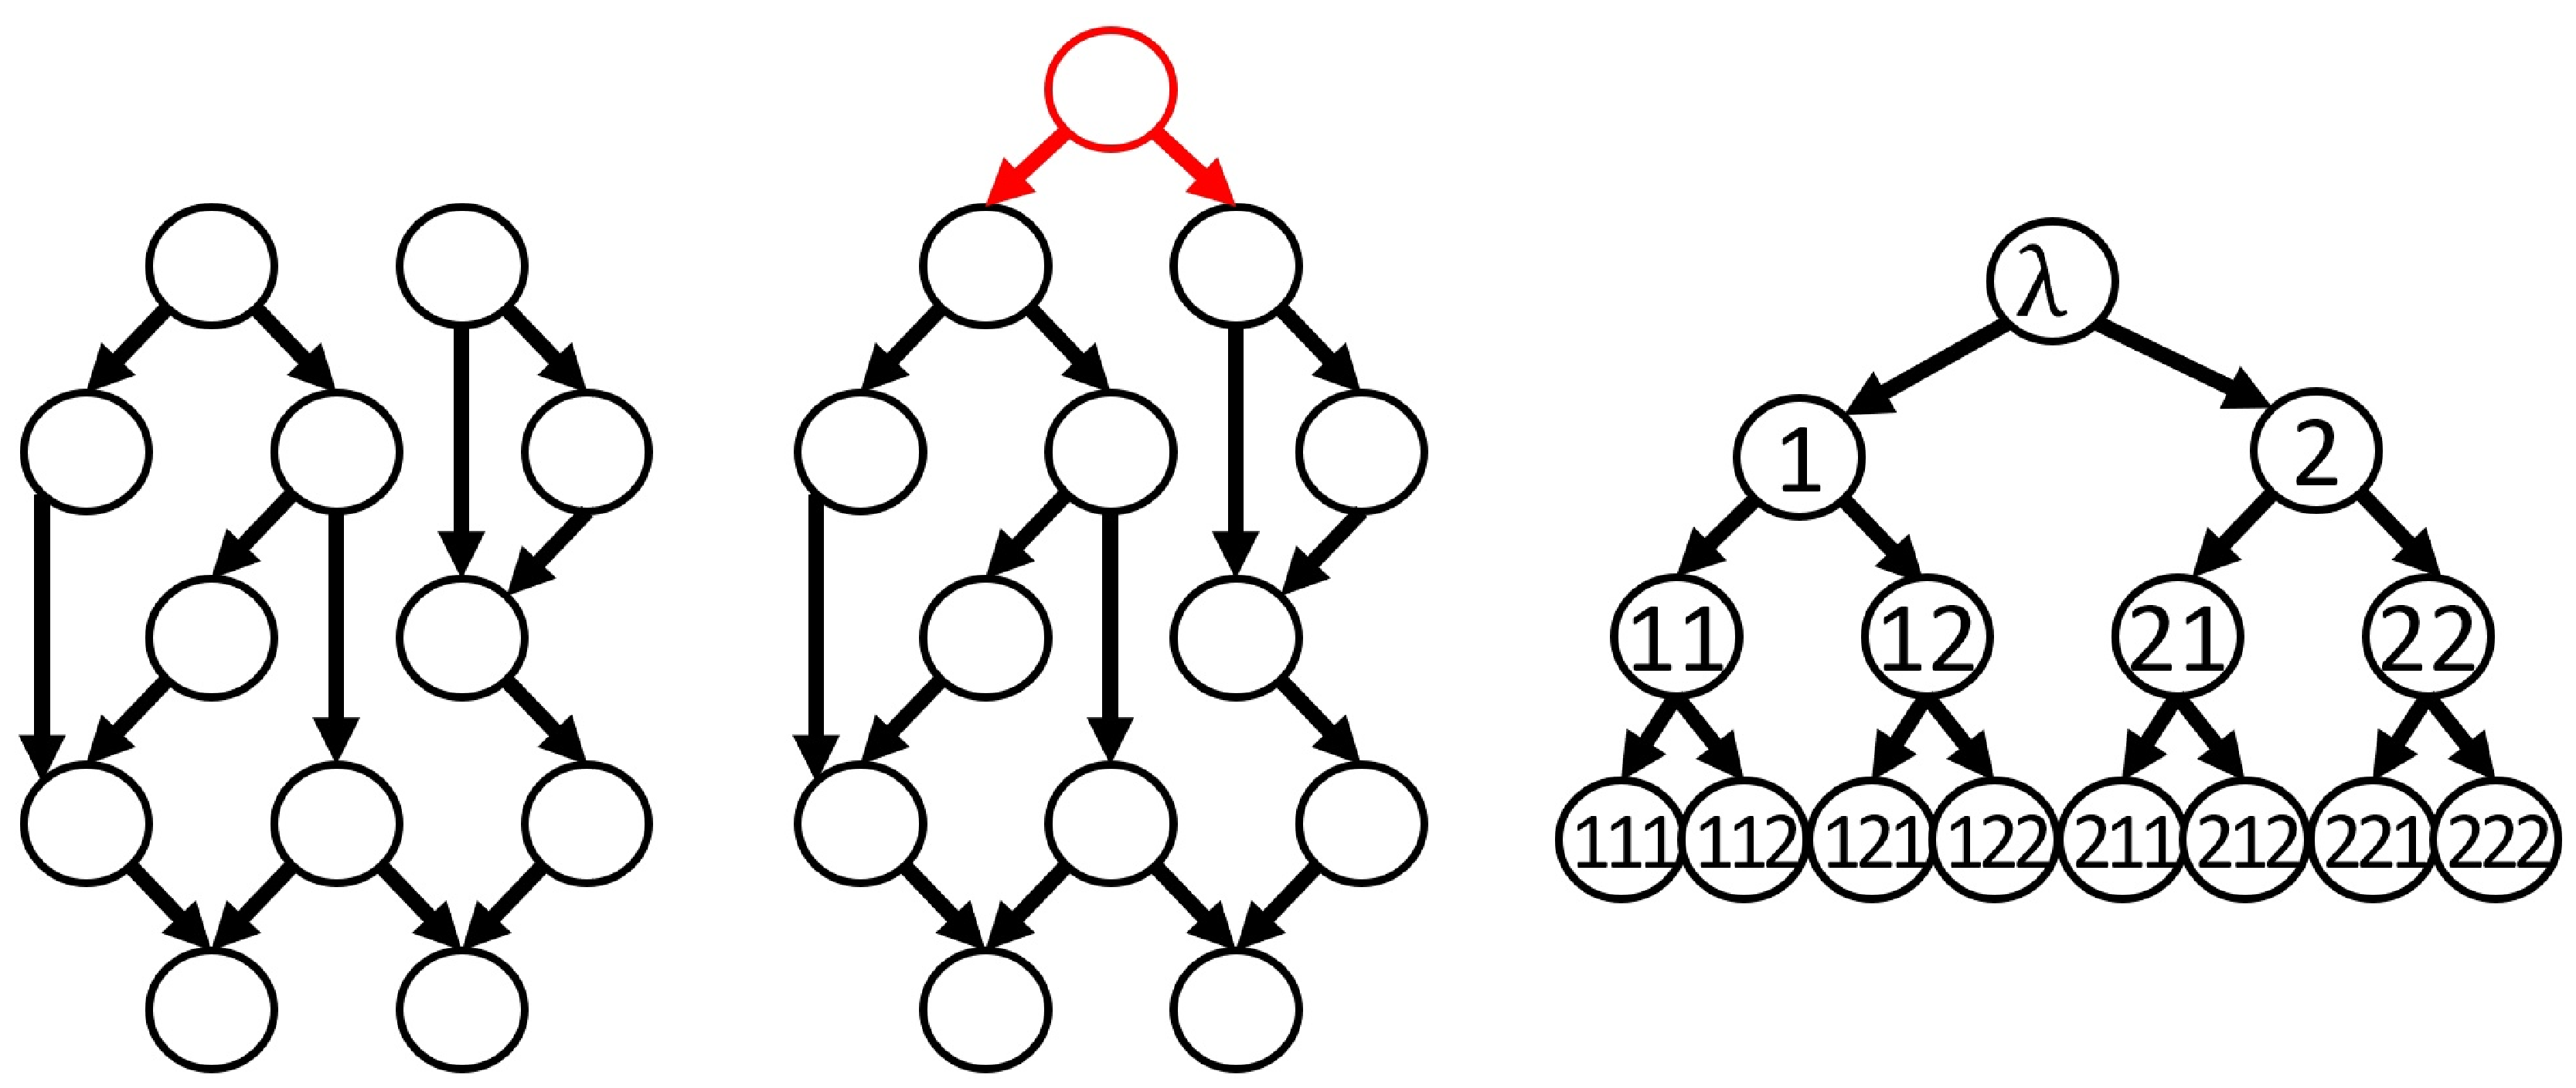
\includegraphics[width=\textwidth]{pic10.eps}
    \caption{given $H$ with $d=2, l=2$ (left) and $t=1$, the construction of $H'$ (center) and $M_{t, d, l}$ (right). $H'$ is obtained by adding a complete directed $d$-ary tree (red part) connected to each root of $H$. Moreover, the labeling of $M_{t, d, l}$ is constructed recursively by appending one character to the right of the parent's label.}
    \label{fig:10}
\end{figure}
}


\ifthenelse{\boolean{Draft}}{
\begin{figure}[H]
    \centering
    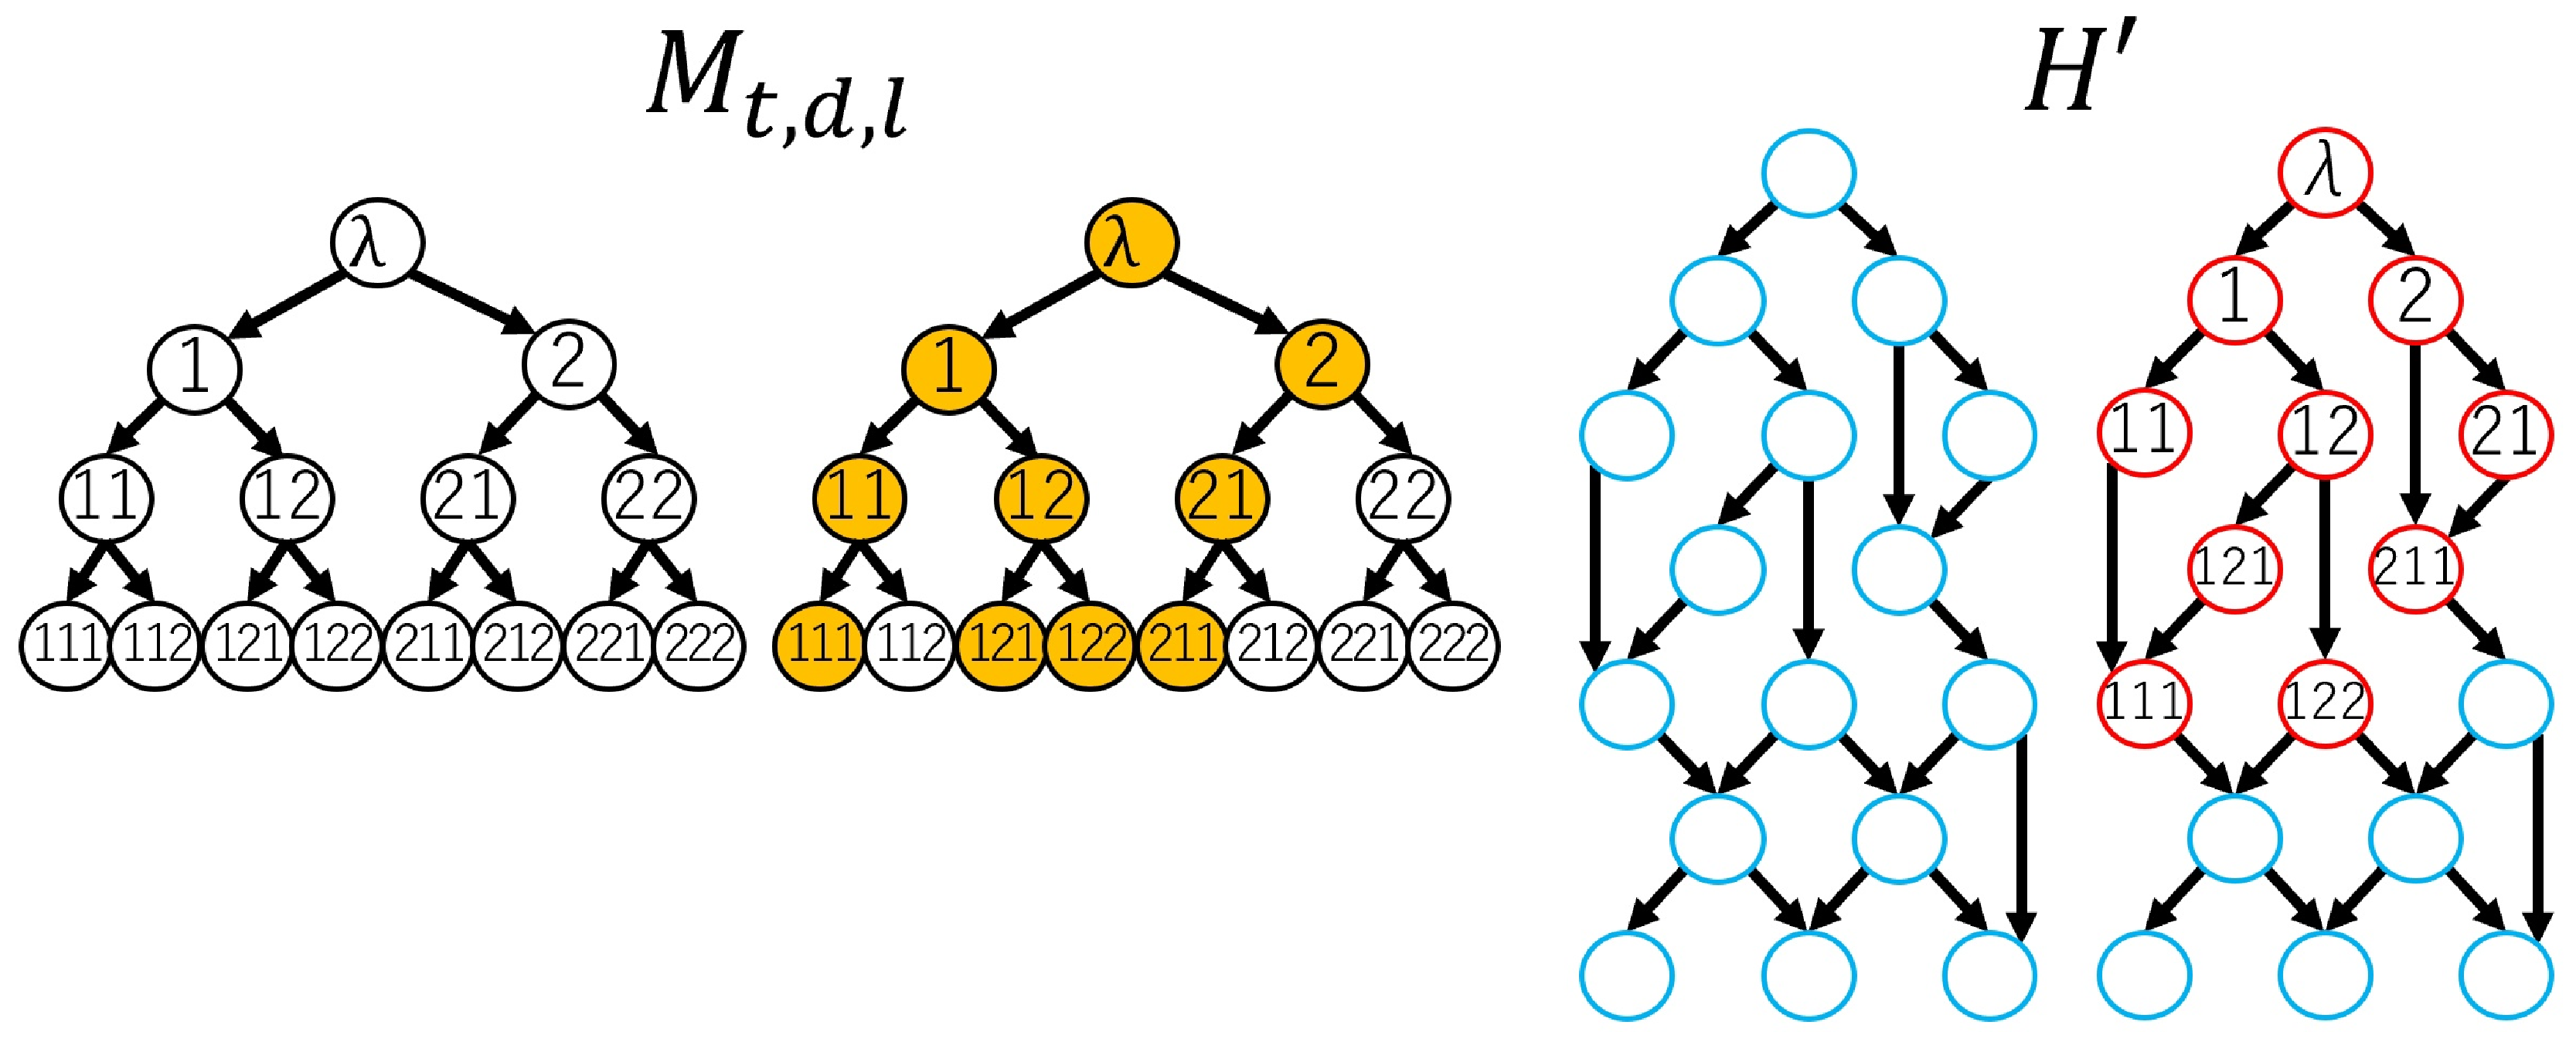
\includegraphics[width=\textwidth]{pic11.eps}
    \caption{Illustration of the operation of $\mathsf{GrowTokenTree}$. The orange tokens in $M_{t, d, l}$ indicate \textit{tokened} tokens. Starting from each left state and ending with each right state. $\mathsf{GrowTokenTree}$ places tokens of $M_{t, d, l}$ onto vertices of $H'$ while preserving the tree structure}
    \label{fig:11}
\end{figure}
}


\ifthenelse{\boolean{Draft}}{
\begin{figure}[H]
    \centering
    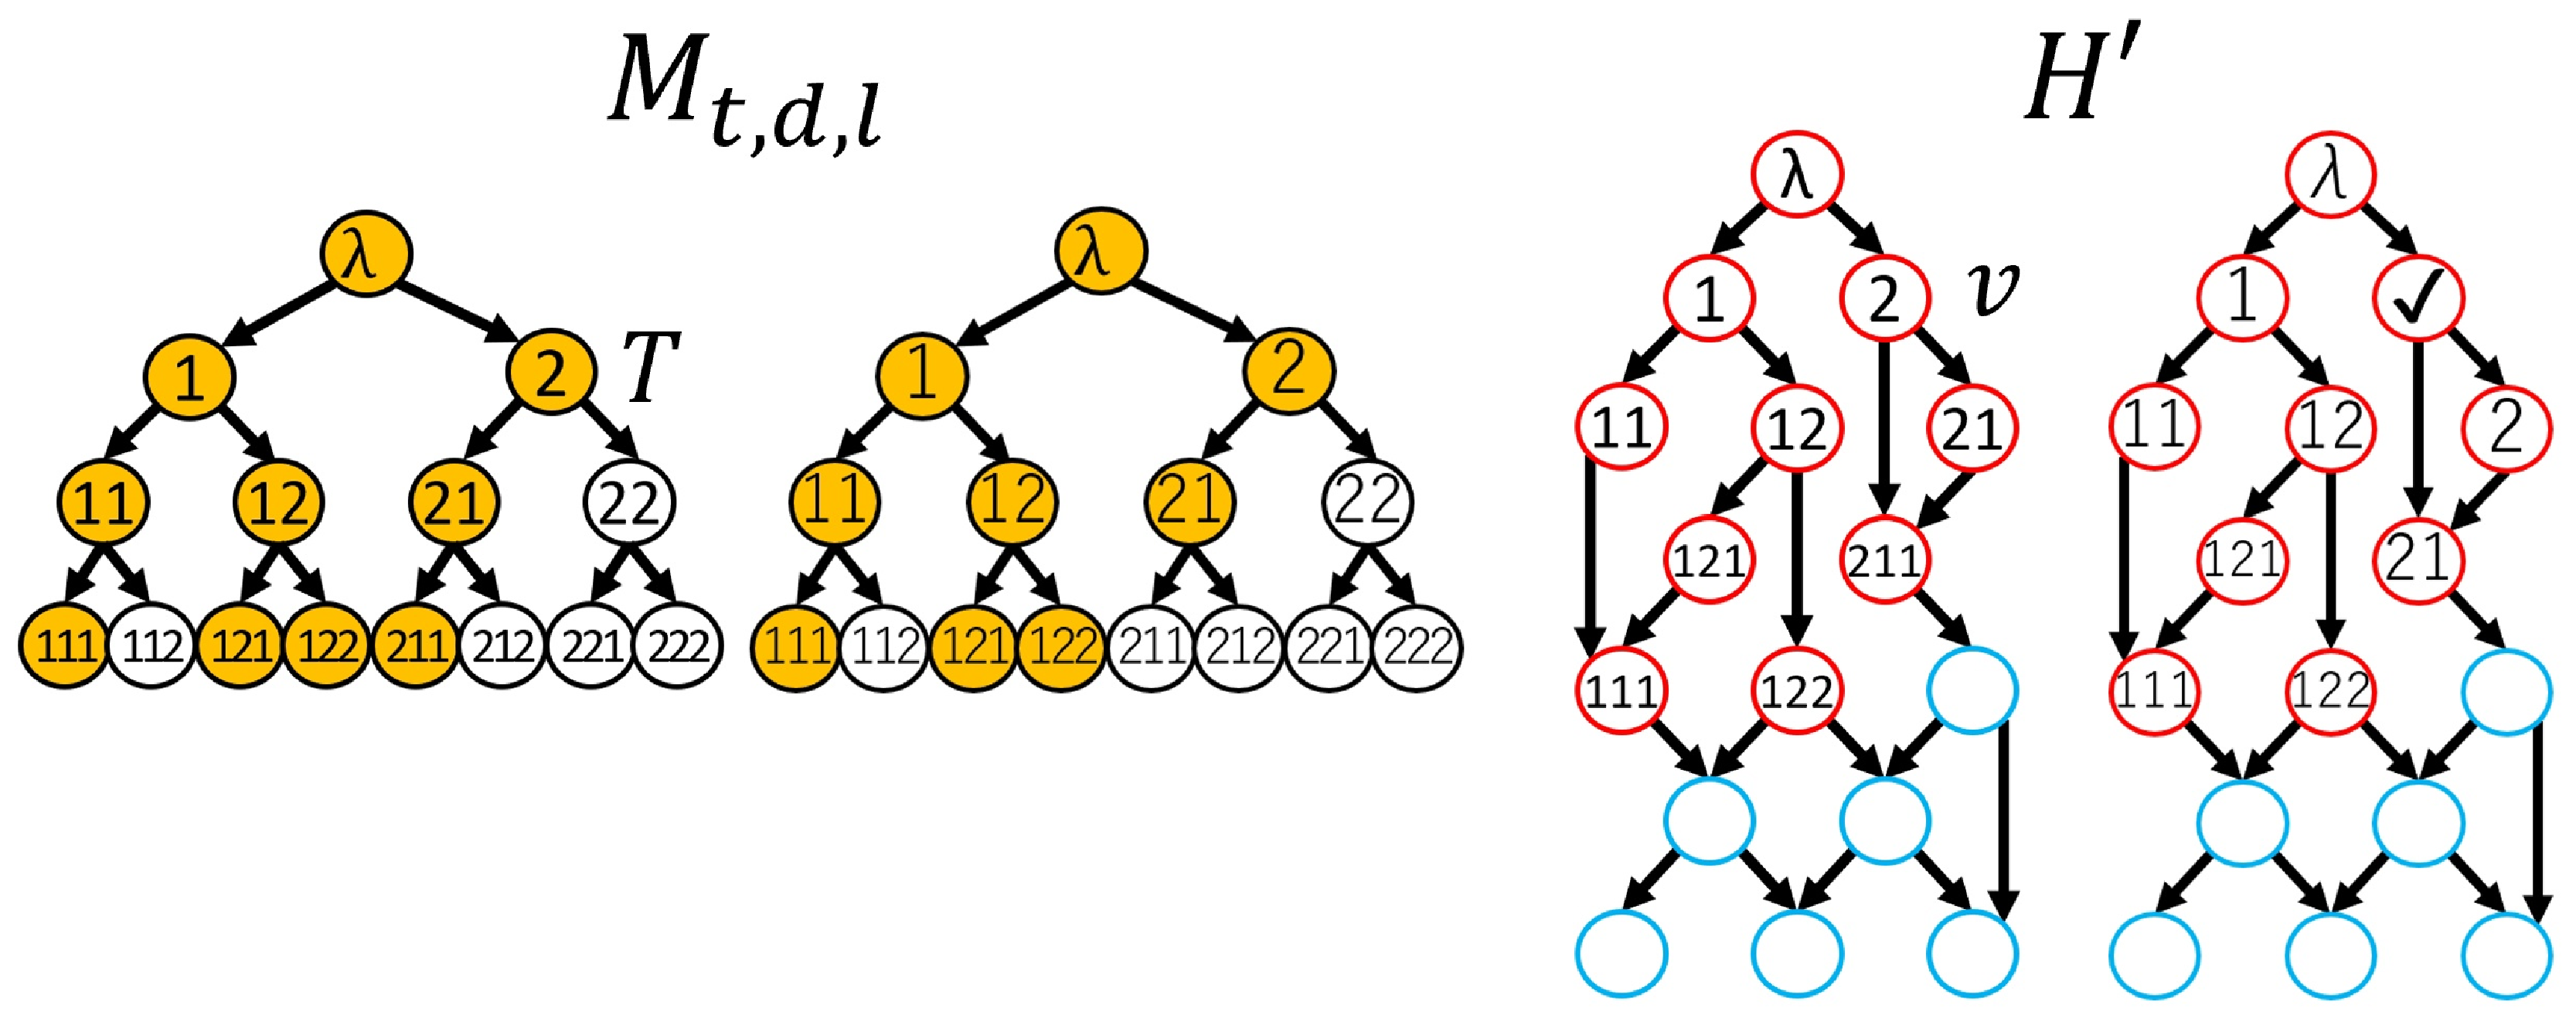
\includegraphics[width=\textwidth]{pic12.eps}
    \caption{Illustration of token replacement in $\mathsf{FindEmbedding}$. A vertex $v$ satisfying the condition in line 5 of the pseudocode (Algorithm \ref{findEmbedding}) and the token $T$ placed at $v$ are selected ($M_{t, d, l}$ left, $H'$ left), and $T$ is removed from $v$. Subsequently, $T$'s all \textit{tokened} descendants $T\cdot b \cdot S$ ($1 \leq b \leq d$ and $S$ is a string of arbitrary length) are replaced with $T \cdot S$ on $H'$.}
    \label{fig:12}
\end{figure}
}



\ifthenelse{\boolean{Draft}}{
\begin{figure}[H]
    \centering
    \begin{minipage}[c]{0.48\textwidth}
        \centering
        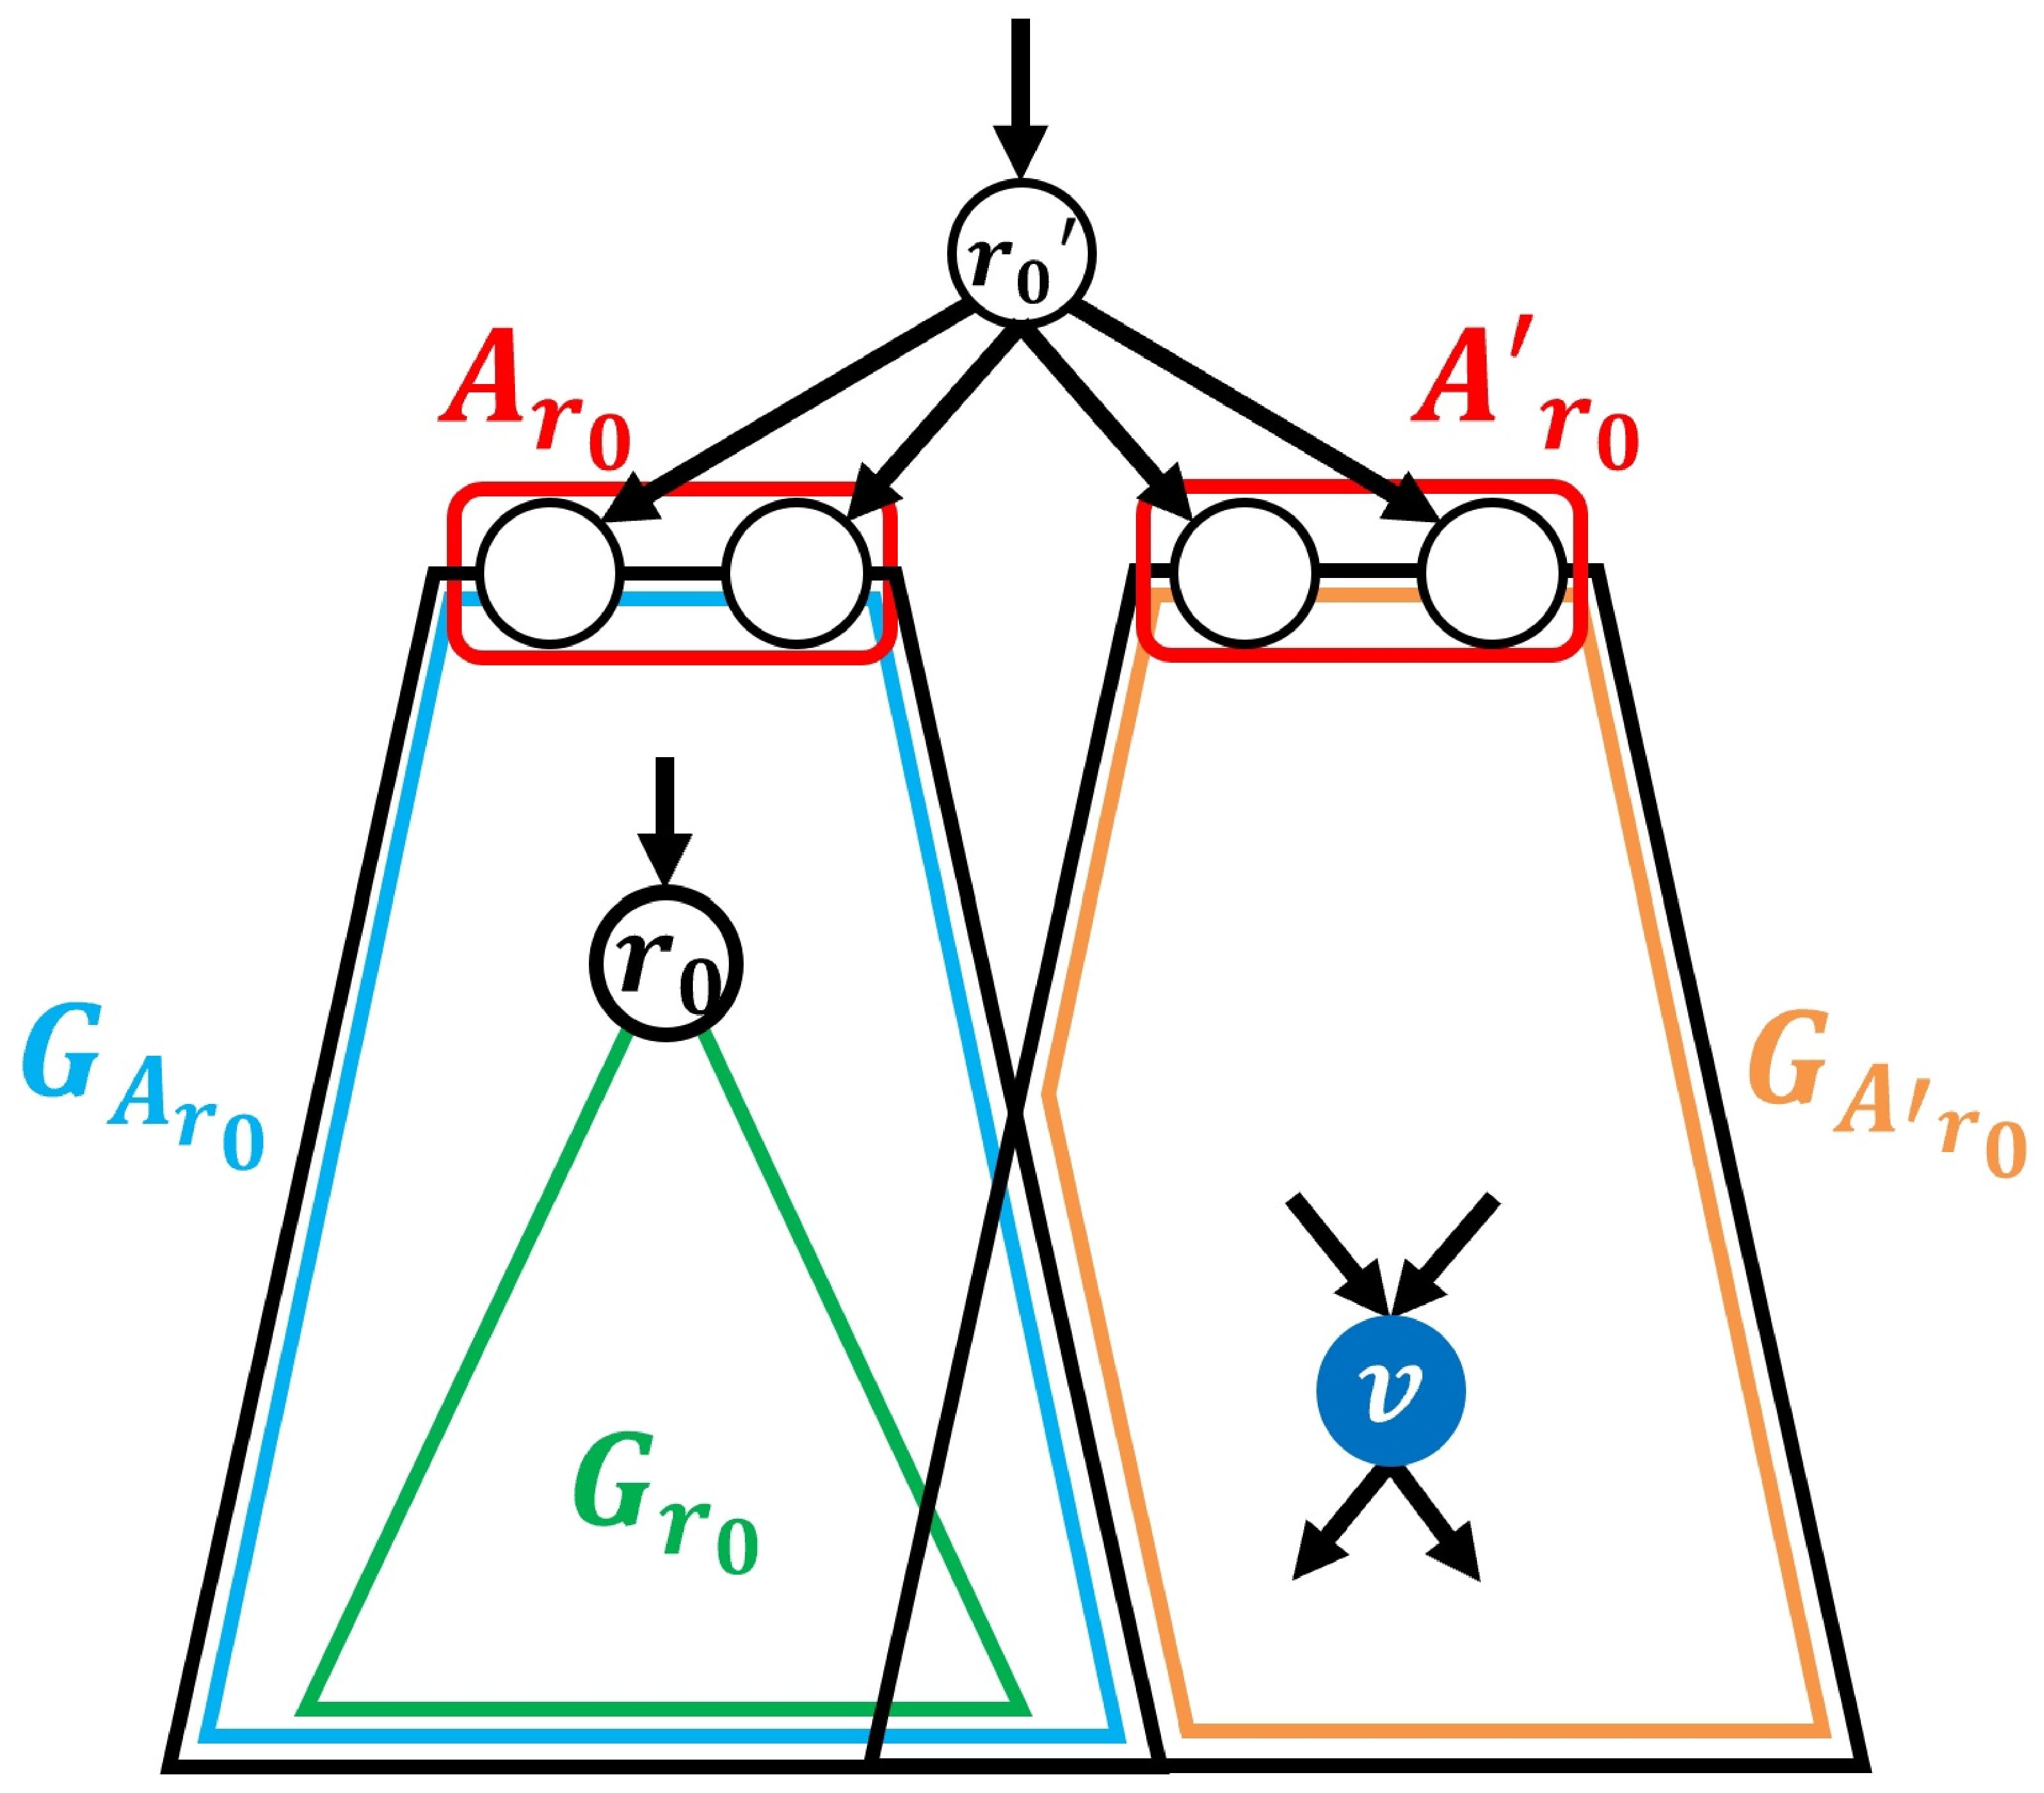
\includegraphics[width=6cm]{pic13.eps}
        \vspace{2.6cm}
        \caption{Illustration of the proof of \textbf{Lemma~\ref{blue_reachable}}. The recent common descendant of $r_0$ and $v$ is denoted as $r_0'$. The proof demonstrates that a contradiction arises if the blue vertex $v$ is not included in $G_{r_0}$, which consists of $r_0$ and its descendants.}
        \label{fig:13}
    \end{minipage}
    \hfill
    \begin{minipage}[c]{0.48\textwidth}
        \centering
        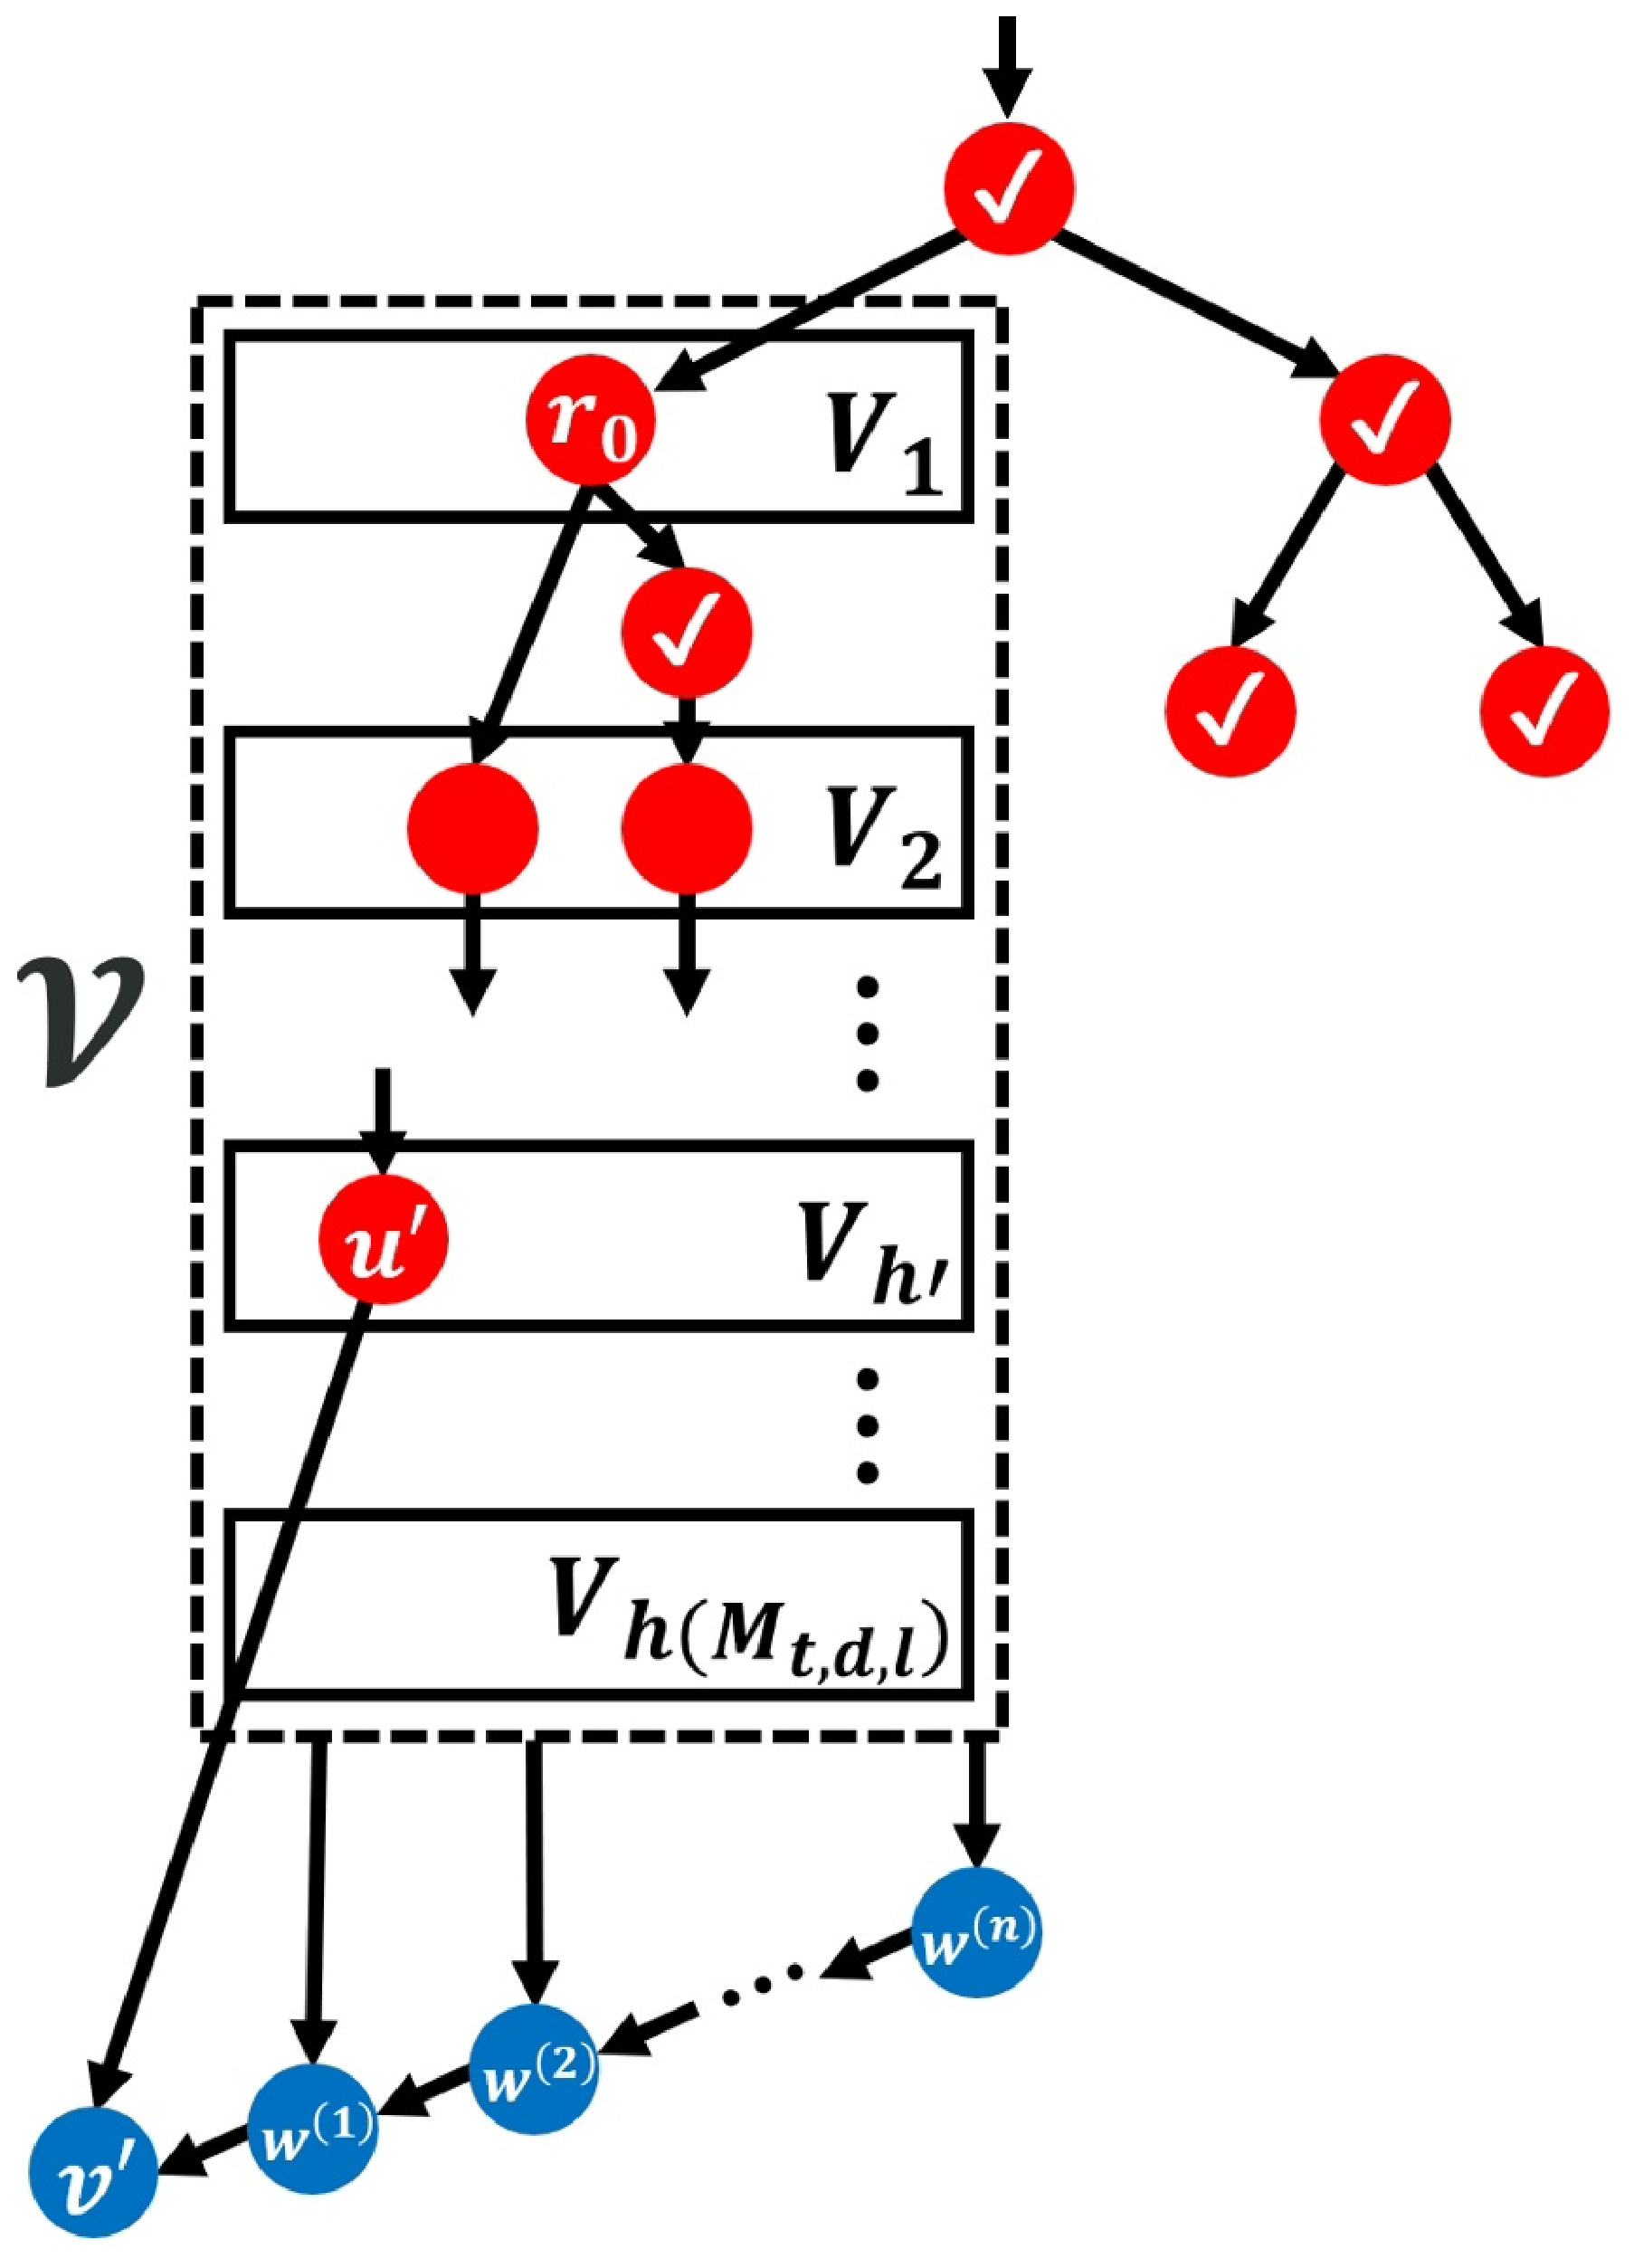
\includegraphics[width=6cm]{pic14.eps}
        \vspace{0.0cm}
        \caption{Illustration of the proof of \textbf{Lemma~\ref{lemma_(3)}}. The blue vertices represent blue, the red check-marked vertices indicate token-removed vertices, and the other red vertices indicate vertices with tokens placed on them. The proof demonstrates that a contradiction arises if there are no vertices in $V_{h(M_{t, d, l})}$.}
        \label{fig:14}
    \end{minipage}
\end{figure}
}








\subsection{\textbf{Lemma~\ref{comp_tree}}}\label{appendix_D2}
\begin{proof}
    We prove this by mathematical induction on $h$. 
    
    For $h=2$, the DAG-pathwidth of $T_{2, d}$ is clearly 1, so the lemma holds. 
    
    Next, assuming that the lemma holds for some $h > 1$, there exists a DAG-path-decomposition $X_h$ of $T_{h, d}$ with DAG-pathwidth $h-1$. Here, note that $T_{h+1, d}$ is a graph obtained by connecting a single root $r$ to the roots of $d$ copies of $T_{h, d}$. We can construct a DAG-path-decomposition of $T_{h+1, d}$ with width $h$ as follows. First, for the $d$ DAG-path-decompositions $X_h$, connect the starting and ending bags of each decomposition sequentially to form a single long sequence of bags. Next, add $r$ to each bag in this sequence. Finally, prepend a bag containing only $r$ at the beginning of the sequence. The resulting sequence satisfies the three rules of a DAG-path-decomposition, making it a valid DAG-path-decomposition of $T_{h+1, d}$ with width $h$.
    
    Furthermore, no DAG-path-decomposition of $T_{h+1, d}$ with width less than $h$ exists. The reasons are shown below. $T_{h+1, d}$ contains $T_{h, d}$ as a substructure, so the DAG-pathwidth of $T_{h+1, d}$ cannot be smaller than $h-1$. Now, suppose there exists a DAG-path-decomposition of $T_{h+1, d}$ with width $h-1$. Since the $d$ copies of $T_{h, d}$ are mutually unreachable, each can independently form a DAG-path-decomposition, and the width does not need to exceed that of a parallel decomposition of the $d$ copies of $T_{h, d}$. Let $T'_{h, d}$ be the first decomposed tree among $d$ $T_{h, d}$. By (DPD2), any DAG-path-decomposition of $T_{h+1, d}$ must include the root $r$ in its first bag. However, the bag in the DAG-path-decomposition of $T'_{h, d}$ that has the maximum width of $h-1$ (denoted as $X'$) does not contain $r$. By (DPD3), $r$ does not reappear in any later bag, implying that the remaining $d-1$ copies of $T_{h, d}$ do not connect to $r$. This requires $d=1$, which contradicts the assumption that $d > 1$. 
    
    Even if all vertices connected to $r$ were included in a bag before $X'$, some vertices from outside $T'_{h, d}$ must necessarily be included in $X'$, which concludes the width greater than $h-1$. It leads to a contradiction.
    
    Thus, no DAG-path-decomposition of $T_{h+1, d}$ with width $h-1$ exists, and the optimal DAG-path-decomposition of $T_{h+1, d}$ has width $h$. Therefore, the lemma holds for $h+1$, and by induction, it holds for any $h, d \geq 2$.
    
\end{proof}


\subsection{\textbf{Lemma~\ref{lemma_embedding}}}\label{appendix_D3}
\begin{proof}
    First, we show that $G'$ is always connected. Token placement and replacement occur only in line 2 of $\mathsf{GrowTokenTree}$ or lines 6 and 8 of $\mathsf{FindEmbedding}$. The former explicitly ensures token placement maintains connectivity, and the latter replaces all tokens in the directed tree rooted at $T \cdot b$ with corresponding tokens in the directed tree rooted at $T$ immediately after removing $T$. This guarantees that connectivity is preserved after processing lines 6 and 8. Thus, $G'$ remains connected at all times.

    Next, we show that an embedding from $G'$ to $H'$ exists. Since $\mathsf{GrowTokenTree}$ places a token $T$ on $u \in V[H']$ and its child $v$ receives token $T \cdot b$, the embedding condition is clearly satisfied. It suffices to verify that the embedding condition holds throughout lines 6 to 9 of $\mathsf{FindEmbedding}$. Assuming that the embedding condition is satisfied at line 5, if a token $T$ satisfying line 5 exists and has exactly one \textit{tokened} child $T \cdot b$, line 8 is executed. In line 8, $S$ represents an arbitrary-length string consisting of characters from $1$ to $d$, and the operation replaces all tokens in the directed tree rooted at $T \cdot b$ with corresponding tokens in the directed tree rooted at $T$ while maintaining tree-structural integrity. Since the replacement occurs from root-proximal tokens to distal ones, the target tokens are always \textit{untokened}. As $G'$ remains connected and $T$ has only $T \cdot b$ as its \textit{tokened} child, removing $T$ and replacing all tokens in the directed tree rooted at $T \cdot b$ with the corresponding tokens in the directed tree rooted at $T$ preserves the embedding condition. If $T$ has no \textit{tokened} children, only line 6 is executed, and line 8 is skipped, trivially maintaining the embedding condition. Thus, the embedding condition remains intact throughout the sequence of operations, proving the existence of an embedding from $G'$ to $H'$.
\end{proof}



\subsection{\textbf{Lemma~\ref{lemma_(1)}}}\label{appendix_D4}
\begin{proof}
    Suppose that in line 4 of $\mathsf{FindEmbedding}$, all vertices of $H'$ have turned red at step $i=s$, leading to termination. The sequence of vertex sets output by the algorithm, $X_{H'} = (X_1, X_2, \dots , X_s)$, constitutes a DAG-path-decomposition of $H'$. Since every vertex $v \in H'$ is red, it must be contained in at least one vertex set $X_i$, satisfying (DPD1). Moreover, each vertex $v$ changes color from blue to red exactly once, and tokens are removed from red vertices without being placed again, ensuring that the vertex sets $X_i$ form a connected path, satisfying (DPD3).

    For any edge $(u, v) \in E[H']$, suppose that $v$ changes from blue to red at $i=i_v~ (i_v \leq s)$. By the condition in line 5 of $\mathsf{FindEmbedding}$, a token placed on $u$ is not removed before step $i_v$. Additionally, by the condition in line 1 of $\mathsf{GrowTokenTree}$, all predecessor vertices of $v$ have tokens, implying that $u$ must also be included in $X_i$. Since $v$ is not in $X_{i_v-1}$, we conclude that $u, v \in X_{i_v}$ and $v \notin X_{i_v-1}$, satisfying (DPD2). Therefore, $X_{H'}$ is a DAG-path-decomposition of $H'$.

    Noting that $\lceil \log_d l \rceil < \log_d l +1$, the width of $X_{H'}$ is at most $|V[M_{t, d, l}]| = d^{\lceil \log_d l \rceil +t+2}-1 < ld^{t+3}-1$. Since $X_H = (X_1 \cap V[H], X_2 \cap V[H], \dots , X_s \cap V[H])$ satisfies the three rules of the DAG-path-decomposition for $H$, it follows that $X_H$ is a DAG-path-decomposition of $H$ with width at most $ld^{t+3}-1$. Thus, we obtain a DAG-path-decomposition of $H$ with width at most $ld^{t+3}-1$.
\end{proof}


\subsection{\textbf{Lemma~\ref{lemma_(2)}}}\label{appendix_D5}
\begin{proof}
    Suppose that in line 4 of $\mathsf{FindEmbedding}$, at step $i=s$, the condition $|X_s| = |V[M_{t, d, l}]|$ holds, and let $A'$ be the subgraph of $H'$ induced by the vertex set $X_1 \cup X_2 \cup \dots \cup X_s$. Then, the sequence of vertex sets output by the algorithm, $X_{A'} = (X_1, X_2, \dots , X_s)$, forms a DAG-path-decomposition of $A'$. By definition of $A'$, (DPD1) is clearly satisfied. Additionally,(DPD2) and (DPD3) are satisfied by the argument similar to \textbf{Lemma~\ref{lemma_(1)}}. Thus, $X_{A'}$ is a DAG-path-decomposition of $A'$.

    Let $A$ be the subgraph of $H$ induced by $V[A'] \cap V[H]$ and $B$ be the subgraph of $H$ induced by $V[H] \backslash V[A]$. Since $A$ and $B$ are disjoint and (DPD2) ensures that only edges from $A$ to $B$ exist. Defining $X_A = (X_1 \cap V[H], X_2 \cap V[H], \dots , X_s \cap V[H])$, this decomposition satisfies the three rules of the DAG-path-decomposition of $A$. Therefore, $X_A$ forms a DAG-path-decomposition of $A$ with width at most $ld^{t+3}-1$ by the argument similar to \textbf{Lemma~\ref{lemma_(1)}}.

    Next, let $A'_M$ be the subgraph of $H'$ induced by the end bag $X_s$ in $X_{A'}$. Since at step $i=s$, all tokens in $M_{t, d, l}$ have been used in the embedding, \textbf{Lemma~\ref{lemma_embedding}} implies that $A'_M$ represents an embedding of $M_{t, d, l}$ into $H'$. Since $M_{t, d, l}$ has height $\lceil \log_d l \rceil +t+2$, and $A'$ contains $A'_M$, the subgraph induced by $V[A'] \backslash V[A]$ forms a complete directed $d$-ary tree of height at most $\lceil \log_d l \rceil$. Thus, $A$ contains a complete directed $d$-ary tree $T_A$ of height at least $(\lceil \log_d l \rceil +t+2) - (\lceil \log_d l \rceil) = t+2$, meaning that an embedding from $T_A$ to $A$ exists. 

    By \textbf{Lemma~\ref{comp_tree}}, the DAG-pathwidth of $T_A$ is $t+1$, implying that the DAG-pathwidth of $A$ is at least $t+1$. Since $H$ contains $A$ as a subgraph, the DAG-pathwidth of $H$ must be greater than $t$. Consequently, the DAG-pathwidth of $A$ is greater than $t$ but at most $ld^{t+3}-1$.
\end{proof}


\subsection{\textbf{Lemma~\ref{blue_reachable}}}\label{appendix_D6}
\begin{proof}
    We prove this by contradiction. Suppose at time $i = k$, there exists a blue vertex $v \in V[H']$ that does not have $r_0$ as an ancestor. Since $H'$ has a single root, there exists a common ancestor of $r_0$ and $v$. Let $r'_0$ be such a most recent common ancestor that does not have another common ancestor of $r_0$ and $v$ as its descendant. If multiple such vertices exist, choose one of them as $r'_0$. Notice that $v \neq r'_0$ because at time $i = k$, the root token $\lambda$ is placed at $r_0$, implying that its ancestor $r'_0$ must have had its token removed. Assuming $r'_0 = v$ contradicts the fact that $v$ is blue.
    
    Define $A_{r_0}$ as the set of children of $r'_0$ whose descendants include $r_0$, and let $A'_{r_0}$ be the set of other children of $r'_0$. Let $G_{A_{r_0}}$ be the subgraph induced by the descendants of the vertices in $A_{r_0}$ and $G_{A'_{r_0}}$ be the subgraph induced by the descendants of the vertices in $A'_{r_0}$ that are not in $G_{A_{r_0}}$. Additionally, let $G_{r_0}$ be the subgraph induced by the descendants of $r_0$. By assumption, $v \notin V[G_{r_0}]$, meaning $v \in V[G_{A_{r_0}}] \setminus V[G_{r_0}]$ or $v \in V[G_{A'_{r_0}}]$ (see Figure~\ref{fig:13} in Appendix~\ref{location_figures}).
    
    Consider the first moment $i = l$ $(l \leq k)$ when a token $\lambda$ is placed on a vertex in $G_{A_{r_0}}$. At this moment, all vertices in $G_{A'_{r_0}}$ must have had their tokens removed. We justify this below. Any vertex in $H'$ is either (a) blue, (b) red with a token, or (c) red and a token is already removed. Since $v$ is blue at $i = l$, Line 5 of $\mathsf{FindEmbedding}$ requires that its parent must be (a) or (b). If the parent is (a), we continue checking its parent, which must also be (a) or (b). If all ancestors of $v$ are (a), at least one blue vertex exists in $A'_{r_0}$ at $i = l$, contradicting the conditions of Line 5. If at least one ancestor is (b), then, when an token $T_{r'_0}$ placed on $r'_0$ has been removed, $T_{r'_0}$ must have had at least two \textit{tokened} children, one in $G_{A'_{r_0}}$ and another elsewhere. Since $T_{r'_0}$ has been removed from $r'_0$ at $i = l$, this contradicts Line 5 of $\mathsf{FindEmbedding}$ which requires that a removed token has at most one \textit{tokened} child. Therefore, $v \notin V[G_{A'_{r_0}}]$ must hold. Given that $v \notin V[G_{A_{r_0}}]$ by assumption, it must hold that $v \in V[G_{A_{r_0}}] \setminus V[G_{r_0}]$. However, in this case, a common ancestor of $v$ and $r_0$ must be included in $A_{r_0}$, which contradicts the fact that there exists no common ancestor of $v$ and $r_0$ among the descendants of $r'_0$. Thus, the claim of \textbf{Lemma~\ref{lemma_(3)}} is proven.
\end{proof}



\subsection{\textbf{Lemma~\ref{lemma_(3)}}}\label{appendix_D7}
\begin{proof}
    Suppose that Line 11 of $\mathsf{FindEmbedding}$ is executed at $i = k$. First, we prove that at $i = k$, there exists at least one root-to-leaf path $P = (\lambda \cdot m_1 \cdot m_2 \cdot \dots m_{\lceil \log_d l \rceil +t+1})$ in the \textit{tokened} token set on $M_{t, d, l}$. Therefore, we show a contradiction by assuming that such a path does not exist. Let $P'$ be the longest path in the \textit{tokened} token set rooted at $\lambda$, and let the height of $M_{t, d, l}$ be $h(M_{t, d, l}) = \lceil \log_d l \rceil +t+2$. By assumption, $|P'| \leq h(M_{t, d, l}) - 1$. Let $T'$ be the terminal token of $P'$, placed at vertex $u' \in V[H']$. From Line 1 of $\mathsf{GrowTokenTree}$, at least one of the following must hold:
    
    \begin{enumerate}
        \item There exists a vertex $v' \in \mathsf{suc}(u')$ such that one of its parents $w^{(1)}$ is blue. \label{cond11}
        \item $T'$ has no \textit{untokened} children. \label{cond22}
    \end{enumerate}
    
    Note that we do not need to consider the case where $u'$ has no children, because in this case, we can remove the token placed on $u'$, preventing the state described in (3) from occurring. If condition \ref{cond22} holds, then $T'$ is either a leaf or all of $T'$'s children are \textit{tokened}. However, neither of these conditions can hold, because by assumption, the endpoint $T'$ of $P'$ is not a leaf, and if $T'$ has a \textit{tokened} child, it would contradict the fact that $P'$ is the longest path. Therefore, condition \ref{cond11} must hold. Let $r_0$ be the vertex where the root token $\lambda$ is placed. Let $G_{r_0}$ be the subgraph induced by the descendants of $r_0$ in $H'$, and let $V_h$ be the set of vertices in $G_{r_0}$ where tokens with height $h\ (1 \leq h \leq h(M_{t, d, l}))$ on the $M_{t, d, l}$ graph are placed . Also, let $\mathcal{V} = \bigcup_{1 \leq h \leq h(M_{t, d, l})} V_h$. By assumption, $u' \in V_{h'}\ (1 \leq h' \leq h(M_{t, d, l})-1)$. Furthermore, by \textbf{Lemma~\ref{blue_reachable}}, both the blue vertices $v', w^{(1)}$ are reachable from $r_0$, so they are contained in $G_{r_0}$. Additionally, considering the placement of tokens in $\mathsf{GrowTokenTree}$, we observe that the children of a blue vertex cannot be red, meaning that $v', w^{(1)}$ and their descendants are not in $\mathcal{V}$. Now, for $w^{(1)}$, one of the following must always hold:

\begin{enumerate}
    \item All of $w^{(1)}$'s parents are in $\mathcal{V}$. \label{cond_a}
    \item There exists at least one blue parent of $w^{(1)}$ that is not in $\mathcal{V}$. \label{cond_b}
\end{enumerate}

    Note that there are no red parents of $w^{(1)}$ that are not in $\mathcal{V}$. This is because, by a similar argument to \textbf{Lemma~\ref{blue_reachable}}, each of $w^{(1)}$'s parents must either be (a) blue or (b) red with a token. Thus, if any parent satisfies (a), condition \ref{cond_b} holds; otherwise, condition \ref{cond_a} holds. If condition \ref{cond_a} holds, a token should be placed on $w^{(1)}$. This is because each of $w^{(1)}$'s parents must be included in one of $V_1, V_2, \dots, V_{h'}$, and each parent has exactly $d$ children, the maximum outdegree in $H'$. Therefore, each parent must have at least one \textit{untokened} child, and this token can be placed on $w^{(1)}$. Thus, the condition \ref{cond_a} contradicts the assumption that $w^{(1)}$ is blue. Therefore, condition \ref{cond_b} must hold. 
    
    If condition \ref{cond_b} holds for $w^{(1)}$, let $w^{(2)}$ be one of blue parents of $w^{(1)}$ satisfying condition \ref{cond_b}. By similar reasoning, a blue parent $w^{(3)}$ of $w^{(2)}$ satisfying condition \ref{cond_b} must exist. Repeating this argument, since the number of vertices in $H'$ is finite, there must eventually be a blue vertex $w^{(n)}$ that satisfies condition \ref{cond_a}. Therefore, a contradiction arises, and there must be at least one path from the root to a leaf in the \textit{tokened} token set on $M_{t, d, l}$ (see Figure~\ref{fig:14} in Appendix~\ref{location_figures}).
    
    Next, we will show that the DAG-pathwidth of $H$ is greater than $t$ using the path $P$. Since there are no tokens satisfying the condition of row 5 in $\mathsf{FindEmbedding}$ in (3), for each token $m_i \in P$ (where $\lambda$ is denoted by $m_0$), the vertex $v_i \in V[H']$ where the token $m_i$ is placed must satisfy at least one of the following:
    
    \begin{enumerate}
        \item There exists a vertex $w_i \in \mathsf{suc}(v_i)$ such that $w_i$ and all its descendants are not in $\mathcal{V}$, and $w_i$ is blue. \label{cond1}
        \item The token placed on $v_i$ has two or more \textit{tokened} children. \label{cond2}
    \end{enumerate}
    
    Next, for each $v_i$, we will show that there exists a vertex $u_i$ such that in any DAG-path-decomposition of $H'$, each $u_i$ (for $0 \leq i \leq h(M_{t, d, l})-1$) must be included in some bag. First, consider the case where $v_i$ satisfies condition \ref{cond1}. In this case, $v_i$ cannot be forgotten in the DAG-path-decomposition of $H'$ until $m_{h(M_{t, d, l})-1}$ is placed at $v_{h(M_{t, d, l})-1}$. This is because $w_i$ and all of its descendants are not included in $\mathcal{V}$, and by taking note of the operation of $\mathsf{GrowTokenTree}$, a token is placed on $w_i$ only after the token $m_{h(M_{t, d, l})-1}$ is placed on $v_{h(M_{t, d, l})-1}$. Since $v_i$, which has $w_i$ as a predecessor, cannot remove $m_i$ before that, $v_i$ cannot be forgotten before the introduction of $v_{h(M_{t, d, l})-1}$ in the DAG-path-decomposition of $H'$. At this point, we set $u_i = v_i$. 
    
    Next, consider the case where $v_i$ does not satisfy condition \ref{cond1} but satisfies condition \ref{cond2}.  
    $m_i$ has at least one \textit{tokened} child $m'_{i+1}$ other than $m_{i+1}$.  
    Since the vertex on which $m'_{i+1}$ is placed also satisfies at least one of conditions \ref{cond1} or \ref{cond2}, by repeating the above argument, and noting that any \textit{tokened} leaf of $M_{t, d, l}$ must satisfy condition \ref{cond1}, there exists at least one descendant vertex of $v_i$ which is placed a descendant token of $m'_{i+1}$ and satisfies condition \ref{cond1}. Let such a vertex be $u_i$.  
    
    For the same reason as above, $u_i$ cannot be forgotten in the DAG-path-decomposition of $H'$ until $m_{h(M_{t, d, l})-1}$ is placed on $v_{h(M_{t, d, l})-1}$. Thus, for each $v_i$, we can construct a corresponding $u_i$.  
    
    In any DAG-path-decomposition $X'$ of $H'$, since each $u_i$ is included in the bag where $v_{h(M_{t, d, l})-1}$ is introduced, the width of $X'$ is at least $h(M_{t, d, l})-1$. Let $P_H$ be the sequence of tokens placed at vertices in $H$ from the sequence $P$. Since $|P \backslash P_H| \leq \lceil \log_d l \rceil$, we have $|P_H| = |P| - |P \backslash P_H| \geq (\lceil \log_d l \rceil + t + 2) - \lceil \log_d l \rceil = t + 2$. Thus, by the same reasoning, the width of any DAG-path-decomposition of $H$ is greater than $t$.
\end{proof}



\subsection{\textbf{Theorem~\ref{approximation3}}}\label{appendix_D8}
\begin{proof}
    By inputting the DAG $H$ into $\mathsf{FindEmbedding}$, the algorithm will always terminate in one of the cases (1), (2), or (3). If it terminates in case (1), by \textbf{Lemma~\ref{lemma_(1)}}, \textbf{Theorem~\ref{approximation3}}(a) holds. If it terminates in case (2), by \textbf{Lemma~\ref{lemma_(2)}}, \textbf{Theorem~\ref{approximation3}}(b) holds. If it terminates in case (3), by \textbf{Lemma~\ref{lemma_(3)}} and setting $A = H$, \textbf{Theorem~\ref{approximation3}}(b) holds. Therefore, \textbf{Theorem~\ref{approximation3}} is proven.
\end{proof}


\subsection{\textbf{Corollary~\ref{cor}}}\label{appendix_D9}
\begin{proof}
    By \textbf{Theorem~\ref{approximation3}}, $\mathsf{FindEmbedding}$ either outputs evidence that the DAG-pathwidth of $H$ is greater than $t$, or outputs a DAG-path-decomposition of width $O(ld^t)$. We now show that $\mathsf{FindEmbedding}$ terminates in polynomial time. In $\mathsf{GrowTokenTree}$, the condition check of line 1 takes $O(dn)$ time, and the while loop is repeated at most $|V[M_{t, d, l}]| = O(d^t)$ times. Also, due to the removal of $T$ in line 6 of $\mathsf{FindEmbedding}$, the vertices where $T$ was placed remain red, so this operation is performed $O(n)$ times. Therefore, the while loop in line 4 is also repeated $O(n)$ times. Furthermore, the while loop in line 10 clearly repeats at most $d^2$ times. Other steps are processed in $O(1)$ time. Thus, the algorithm terminates in $O(n^2)$ time if $d$ and $l$ are bounded by constants.
\end{proof}











\begin{comment}
    
\subsection{A Subsection Sample}
Please note that the first paragraph of a section or subsection is
not indented. The first paragraph that follows a table, figure,
equation etc. does not need an indent, either.

Subsequent paragraphs, however, are indented.

\subsubsection{Sample Heading (Third Level)} Only two levels of
headings should be numbered. Lower level headings remain unnumbered;
they are formatted as run-in headings.

\paragraph{Sample Heading (Fourth Level)}
The contribution should contain no more than four levels of
headings. Table~\ref{tab1} gives a summary of all heading levels.

\begin{table}
\caption{Table captions should be placed above the
tables.}\label{tab1}
\begin{tabular}{|l|l|l|}
\hline
Heading level &  Example & Font size and style\\
\hline
Title (centered) &  {\Large\bfseries Lecture Notes} & 14 point, bold\\
1st-level heading &  {\large\bfseries 1 Introduction} & 12 point, bold\\
2nd-level heading & {\bfseries 2.1 Printing Area} & 10 point, bold\\
3rd-level heading & {\bfseries Run-in Heading in Bold.} Text follows & 10 point, bold\\
4th-level heading & {\itshape Lowest Level Heading.} Text follows & 10 point, italic\\
\hline
\end{tabular}
\end{table}

\noindent Displayed equations are centered and set on a separate
line.
\begin{equation}
x + y = z
\end{equation}
Please try to avoid rasterized images for line-art diagrams and
schemas. Whenever possible, use vector graphics instead (see
Fig.~\ref{fig1}).

\begin{figure}
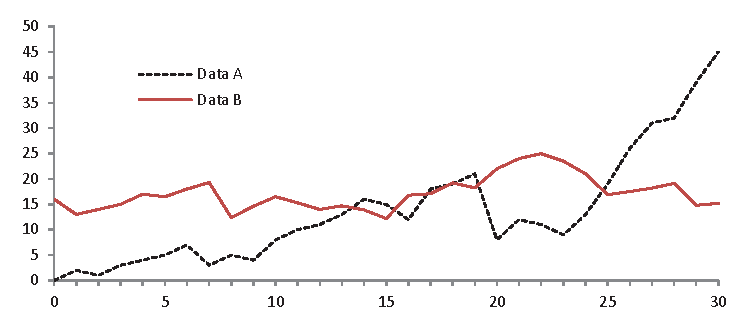
\includegraphics[width=\textwidth]{fig1.eps}
\caption{A figure caption is always placed below the illustration.
Please note that short captions are centered, while long ones are
justified by the macro package automatically.} \label{fig1}
\end{figure}

\begin{theorem}
This is a sample theorem. The run-in heading is set in bold, while
the following text appears in italics. Definitions, lemmas,
propositions, and corollaries are styled the same way.
\end{theorem}
%
% the environments 'definition', 'lemma', 'proposition', 'corollary',
% 'remark', and 'example' are defined in the LLNCS documentclass as well.
%
\begin{proof}
Proofs, examples, and remarks have the initial word in italics,
while the following text appears in normal font.
\end{proof}
For citations of references, we prefer the use of square brackets
and consecutive numbers. Citations using labels or the author/year
convention are also acceptable. The following bibliography provides
a sample reference list with entries for journal
articles~\cite{ref_article1}, an LNCS chapter~\cite{ref_lncs1}, a
book~\cite{ref_book1}, proceedings without editors~\cite{ref_proc1},
and a homepage~\cite{ref_url1}. Multiple citations are grouped
\cite{ref_article1,ref_lncs1,ref_book1},
\cite{ref_article1,ref_book1,ref_proc1,ref_url1}.

\begin{credits}
\subsubsection{\ackname} A bold run-in heading in small font size at the end of the paper is
used for general acknowledgments, for example: This study was funded
by X (grant number Y).

\subsubsection{\discintname}
It is now necessary to declare any competing interests or to specifically
state that the authors have no competing interests. Please place the
statement with a bold run-in heading in small font size beneath the
(optional) acknowledgments\footnote{If EquinOCS, our proceedings submission
system, is used, then the disclaimer can be provided directly in the system.},
for example: The authors have no competing interests to declare that are
relevant to the content of this article. Or: Author A has received research
grants from Company W. Author B has received a speaker honorarium from
Company X and owns stock in Company Y. Author C is a member of committee Z.
\end{credits}

\end{comment}

\end{document}
